%--------------------
% document principal
%--------------------
% cal compilar amb `pdflatex -shell-escape memoria.tex`
%--------------------
\documentclass[a4paper,12pt,twoside,BCOR12mm]{scrbook}
%%%%BCOR12mm  factor de correcció per enquadernació
\usepackage[catalan]{babel}
\usepackage[utf8]{inputenc}
\usepackage[T1]{fontenc} 

 
%---------- Mode esborrany --------------------
%\includeonly{resum}
%\usepackage{fancyhdr}
%\pagestyle{fancyplain}
%\chead{\fancyplain{--- esborrany \today\ ---}{}}
%%\renewcommand{\headrulewidth}{0pt}
%----------------------------------------------



%---------- Bibliografia -------------------
\usepackage[style=numeric,sortcites=true]{biblatex}
\bibliography{bibliografia}
%---------- Gràfics ------------------------
\usepackage[final]{graphicx}
% \graphicspath{{imatges/}}
\usepackage{epstopdf}
\usepackage{tikz}
\usepackage{pgfplots}
%\usepackage[off]{auto-pst-pdf}
\usepackage{epic,color,multicol}
\usepackage{cclicenses}
%---------- Símbols ------------------------
\usepackage{url} %\url i \path
\usepackage{eurosym}
\usepackage{amsmath,amssymb,amsthm}
\numberwithin{equation}{chapter}
\newtheorem{definition}{Definició}
\DeclareMathOperator*{\seg}{seg}
\DeclareMathOperator*{\ant}{ant}
%\usepackage{numprint} %%aleshores \numprint{2,5} sinó es pot utilitzar 2{,}5
%---------- Codi ---------------------------
\usepackage{upquote} %perquè en verbatim surtin les cometes `
\usepackage{listings}
\lstloadlanguages{bash,C,HTML,Python,XML}
\lstset{frame=single,frameround=tttt,escapechar=@,
        breaklines=true,breakindent=0pt,numberstyle=\tiny,
        prebreak=\mbox{{\color{blue}\tiny$\searrow$}},
        postbreak=\mbox{{\color{blue}\tiny$\rightarrow$}},
        columns=fullflexible,
        extendedchars=true,literate={à}{{\`a}}1 {è}{{\`e}}1 {é}{{\'e}}1 {í}{{\'\i}}1 {ï}{{\"\i}}1 {ò}{{\`o}}1 {ó}{{\'o}}1 {ú}{{\'u}}1 {ü}{{\"u}}1 {ç}{{\c{c}}}1 {l·l}{{\l.l}}1
{À}{{\`A}}1 {È}{{\`E}}1 {É}{{\'E}}1 {Í}{{\'\I}}1 {Ï}{{\"\I}}1 {Ò}{{\`O}}1 {Ó}{{\'O}}1 {Ú}{{\'U}}1 {Ü}{{\"U}}1 {Ç}{{\c{C}}}1 {L·L}{{\L.L}}1, 
      }

\lstdefinestyle{sh} 
    {language=sh, frame=none, prebreak =\textbackslash, postbreak ={},basicstyle=\ttfamily,showspaces=false,keepspaces=true}

%% ÚS del lstlisting
%%\begin{lstlisting}[language=C,caption=Plantilla de NagiosGrapher pels missatges,label=NGmis,numbers=left]
%%\lstinline[style=sh]!for i:integer;!
%--------------------------------------------





%------------- format -------------------------
\parindent0cm 
\parskip0.2cm

\usepackage[bookmarks,pdfborder={0 0 0},pdfusetitle,
    pdftitle={Estudi i modelització dels SGBD Round Robin pel tractament de sèries temporals},
    pdfauthor={Aleix Llusà Serra},
    pdfsubject={SGBD RRD},
    pdfkeywords={sèries temporals; adquisició de dades; SGBD per a sèries temporals; model de dades Round Robin (RRD); SGBD RRDtool},
    ]{hyperref}
%----------------------------------------------



\begin{document}

%------------- Pàgina de títol ------------
%\documentclass[11pt,english,a4paper,twoside]{book}

%%%%%%%%%%%%%%%%%%%%%%%%%%%%%%%%%%%%%%%%%%%%%%%%%%%%%%%%%%%%%%%%%%%%%%%%%%%
%\setlength{\textheight}{21.5cm}%
%\setlength{\headsep}{1cm}%
%\setlength{\topmargin}{0cm}%
%\setlength{\headheight}{0.5cm}%
%\setlength{\oddsidemargin}{.4cm}%
%\setlength{\evensidemargin}{-.6cm}%
%\setlength{\textwidth}{16cm}%
%\setlength{\footskip}{1.5cm}%


%\usepackage[english]{babel}
%\usepackage[latin1]{inputenc}




%###########################################################################
%\begin{document}


%------------- capçaleres pdf -----------
\pdfinfo {
/Title (Modelització dels SGBD RRD)
/Author	 (Aleix Llusà Serra) 
/Subject (Estudi i modelització
    dels SGBD
    Round Robin pel tractament de sèries temporals)
/Keywords (sèries temporals; adquisició de dades; SGBD per a sèries temporals; model de dades Round Robin (RRD); SGBD RRDtool)
}

%------------- pàgina de títol -----------
\begin{titlepage}
\begin{center}
{\Large \sc Universitat Polit\`{e}cnica de Catalunya} \vskip 1cm
{M\`{a}ster:} \vskip 0.5cm {\sc Autom\`{a}tica i Rob\`{o}tica} \vskip 4cm {Tesi
de M\`{a}ster} \vskip 1cm {\Large \bf \sc  Estudi i modelització
    dels SGBD
    Round Robin pel tractament de sèries temporals}

\vskip 2cm {\bf Aleix Llusà Serra} \vskip 4cm { Directors:
   Teresa Escobet Canal i 
    Sebastià Vila-Marta}

\vskip 1cm {\large Curs Acad\`{e}mic 2010/11}\\
\vfill {Juny 2011}
\end{center}
\end{titlepage}
%\end{document}



%%% Local Variables: 
%%% mode: latex
%%% TeX-master: "memoria"
%%% End: 

%----------------------------------------------


%------------- Abstract ------------
\chapter*{Resum}

\todo{repassar la taula de notació que a vegades fa un salt de pàgina on no toca}

Actualment és possible d'adquirir una gran quantitat de dades,
principalment gràcies a la facilitat de disposar de sistemes de
monitoratge amb grans xarxes de sensors. Això no obstant, no és tan
senzill de gestionar posteriorment totes aquestes dades.  A més, també
cal tenir en compte com s'emmagatzemen aquestes dades.


D'una banda, l'adquisició de valors d'una variable al llarg del temps
es formalitza com a sèrie temporal. Així, hi ha multitud d'algoritmes
i metodologies d'anàlisi de sèries temporals que descriuen com
extreure informació de les dades. D'altra banda, l'emmagatzematge i la
gestió de les dades es formalitza com a \glspl{SGBD}. Així, hi ha
sistemes informàtics dedicats a inferir la informació que un usuari
vol consultar. Aquests sistemes són descrits per models lògics
formals, entre els quals el model relacional n'és la referència
principal.


En aquesta tesi dissertem sobre el fet d'emmagatzemar només aquella
part de les dades originals que conté una certa informació
seleccionada. Aquesta selecció de la informació es duu a terme
mitjançant el resum de diferents resolucions de les dades, cadascuna
de les quals bàsicament són agregacions de les dades a intervals de
temps periòdics. A aquesta tècnica l'anomenem multiresolució.



La multiresolució s'aplica a les sèries temporals. Com a resultat,
s'obtenen subsèries temporals de mida finita i amb la informació
resumida. Per tal de gestionar les sèries temporals, s'utilitzen
\gls{SGBD} específics anomenats \glspl{SGST}. Així doncs, proposem
\gls{SGST} amb capacitats de multiresolució i els anomenem
\glspl{SGSTM}. De la mateixa manera que en els \gls{SGBD}, formalitzem
un model pels \gls{SGST} i pels \gls{SGSTM}.



A causa de la naturalesa de variable capturada al llarg del temps, en
l'adquisició de les sèries temporals apareixen propietats
problemàtiques. Els \gls{SGSTM} tenen en compte algunes d'aquestes
propietats com:
\begin{itemize}
\item La sincronització dels rellotges en els diferents sistemes
  d'adquisició.
\item L'aparició de dades desconegudes perquè no s'han pogut adquirir
  o perquè són errònies.
\item La gestió d'una quantitat enorme de dades, i que a més segueix
  creixent al llarg del temps.
\item Les consultes amb dades que no s'han recollit de manera uniforme
  en el temps.
\end{itemize}


Ara bé, els \gls{SGSTM} són uns sistemes que emmagatzemen unes dades
segons una selecció d'informació i descarten les que no es consideren
importants. Per tant, prèviament a l'emmagatzematge, cal decidir els
paràmetres de selecció de la informació. Per tal d'avaluar la qualitat
d'aquests sistemes, depenent dels paràmetres que s'escullin, es pot
utilitzar la teoria de la informació. En aquest sentit, la
multiresolució es pot considerar com una tècnica de compressió amb
pèrdua. Així doncs, introduïm una reflexió sobre com avaluar l'error
que es comet amb la multiresolució en comparació amb disposar de totes
les dades originals.


Com es diu actualment en l'àmbit dels \gls{SGBD}, un mateix sistema no
pot ser adequat per a tots els contextos. A més, els sistemes han de
tenir en compte un bon rendiment en altres recursos a part del temps
de computació, com per exemple la capacitat finita, el consum
d'energia o la transmissió per la xarxa. Així doncs, dissenyem
diverses implementacions del model dels \gls{SGSTM}. Aquestes
implementacions exploren diverses tècniques de computació: computació
incremental seguint el flux de dades, computació para\l.lela i
computació de bases de dades relacional.


En resum, en aquesta tesi dissenyem els \gls{SGSTM} i en formalitzem
un model.  Els \gls{SGSTM} són útils per a emmagatzemar sèries
temporals en sistemes amb capacitat finita i per a precomputar la
multiresolució. D'aquesta manera, permeten disposar de consultes i
visualitzacions immediates de les sèries temporals de forma
resumida. Això no obstant, impliquen una selecció de la informació que
cal decidir prèviament. En aquesta tesi proposem consideracions i
reflexions sobre els límits de la multiresolució.





\chapter*{Abstract}






\glsreset{SGBD}
\glsreset{SGST}
\glsreset{SGSTM}


%%% Local Variables: 
%%% mode: latex
%%% TeX-master: "main"
%%% End: 

%  LocalWords:  multiresolució

%----------------------------------------------


%------------- Índexs ------------
\cleardoublepage\pdfbookmark{\contentsname}{bookmark:index}\tableofcontents
%\addtocontents{toc}{\protect\enlargethispage{1cm}}
%\listoffigures
%\listoftables
%\lstlistoflistings
%----------------------------------------------



%------------- Cos ------------

%\mainmatter

\begin{abstract}
  Current monitoring systems are an essential part of supervising
  control as they manage a large amount of information. Data
  collection is normally studied as a time series owing to it fits
  into sequence of values.  Thanks to the facility of designing
  monitoring hardware, the measurement of data has increased the last
  decade and there is not enough capacity to store nor process all the
  time series. Therefore, we need to design database management
  systems capable of storing and processing efficiently the time
  series. Moreover, this systems have to cope with the measurements
  not happening at regular time intervals as it is a restriction
  imposed by some time series treatment algorithms.

  In this paper a formal model for a time series database management
  system is designed.  It is called Multiresoltion Time Series
  Database Management Systems model (MTSMS). A Time series is
  compactly stored in the database and the information is summarised
  by different interpolation functions. From this model this kind of
  DBMS will be better understood, new implementations will be possible
  and we will be able to enhance its potential.
\end{abstract}



\section{Introduction}

This paper focuses on Data Base Management Systems (DBMS) that store
and treat data as time series.  Traditional DBMS, as is ones derived
from relational model, are not adequate for these cases as they do not
have enough facilities to manage and retrieve time series
information \parencite{schmidt95}.

Some DBMS have already taken into account the specificities of time
series, then called Time Series Data Base Management Systems
(TSMS) \parencite{dreyer94}.  Time Series Data
Server \parencite{weigel10} allows to select a data range from a time
series and to apply a filter when the data is retrieved.
RRDtool \parencite{rrdtool} applies filters and stores different data
ranges when data is stored, moreover it considers that the sampling
times can not be equally spaced, the temporal order is essential and
the value and time must be stored together. However, this TSMS lack
the complete definition of the relation between the three main fields
involved: time series, monitoring systems and DBMS.

Monitoring sensor data and processing this data to achieve diagnosis,
prognosis, prediction, data fusion or other time series analysis tasks are common in many fields such as prognosis in degradation models \parencite{yu11}, qualify sensor health in navy vessels \parencite{palmer07}, validate and reconstruct data in water distribution networks \parencite{quevedo10}, sensor networks information dissemination \parencite{deligiannakis07} or economic stock classification \parencite{dreyer95}. Time series data mining formalises the knowledge discovery in time series databases \parencite{last01}. 


DBMS are based from formal models that define the objects and
operations of the abstract machine to which users interact, such is
the relational model \parencite{date}. TSMS lack a consolidated formal
model, although special properties and requirements for a TSMS
have been proposed \parencite{dreyer94}.

In this paper
a model is proposed for an storage system that will keep a time series
in a multiresolution and bounded way.  In this first proposal there
are six definitions that are related to the data storage mechanism:
measure, time series, buffer, disc, resolution disc, and multiresolution
database. Some of this concepts are familiar with RRDtool
operating mode.


\todo{estructura article}
The paper is organised as follows. In \autoref{sec:preliminaries} the preliminaries concerning TSMS are summarised. In \autoref{sec:TSMS} the state of TSMS is shown as well as known similar systems that are designed with some TSMS properties. In \autoref{sec:MTSMS} a model for a multiresolution TSMS is presented for the first time. Possible reference implementations of this model are explored in \autoref{sec:implementation}. In sections \ref{sec:conclusion} and \ref{sec:future}  the MTSMS is concluded and future work is proposed. In \autoref{sec:notation} the main nomenclature and notation used in the paper is summarised. 




%%% Local Variables: 
%%% mode: latex
%%% TeX-master: "article"
%%% ispell-local-dictionary: "british"
%%% End: 


\include{estat}

\chapter[Magnituds i comptadors]{Comparació de magnituds i comptadors}
\label{cap:velocitats}

%%--------------------------
%%Posició de totes les llegendes
\pgfplotsset{every axis legend/.append style={
        at={(0.05,0.95)},
        anchor=north west}}
%%--------------------------

Al capítol~\ref{cap:rrdtool-etapes} s'explica profundament com es tracten les dades a RRDtool fins que queden emmagatzemades. Abans de l'etapa de normalització d'intervals, hi ha una etapa de transformació a velocitat que pot quedar descontextualitzada si no s'expliquen els motius històrics que han portat a tractar les dades d'aquesta manera. 

En aquest capítol es raona per què RRDtool té interès a diferenciar variables que classifica com a comptadors i magnituds i per què aplica l'etapa de transformació a velocitat descrita en detall a l'apartat~\ref{sec:rrdtool-etapes:velocitat}. S'anomena velocitat al flux o taxa de variació dels valors quan són expressats com a ràtio magnitud per unitat de temps.


En la primera versió, RRDtool només s'utilitzava per un sistema que monitorava els comptadors de tràfic de xarxa dels encaminadors (\emph{routers}) i els tractava de manera especial, basant-se en la velocitat mitjana del comptador. 
En el primer apartat es resumeix la idea principal d'aquest tractament de velocitat. 

En evolucions posteriors de RRDtool, aquest tractament s'ha mantingut per totes les dades; és a dir que totes les dades es transformen i s'interpreten com a velocitat, fins i tot les que no són comptadors. Es pot concloure que els comptadors han esdevingut el 'cas bàsic' de RRDtool. En un segon apartat s'analitzen les conseqüències que això comporta per a les dades que es mesuren com a magnituds, per exemple la temperatura. 

Al tercer apartat es detallen els noms que utilitza RRDtool per emmagatzemar les variables classificades com a comptadors i com a magnituds i quines possibilitats ofereix per representar-les.

\section{Comptadors}

Com ja s'ha comentat anteriorment, cal situar els inicis de RRDtool en el monitoratge de xarxa de comunicacions amb comptadors. Aquests comptadors són una variable que es va incrementant monòtonament; és a dir són una funció creixent infinita. Per aquesta particularitat, els anomenem comptadors monòtons.

Quan es pren una mesura d'un comptador monòton s'obté un valor que indica el total de comptatge des de l'inici del comptador; és a dir que sempre es mesura amb referència absoluta. 
Per exemple, en diferents instants de temps es prenen mesures d'un comptador de tràfic de xarxa i s'obté el total de bytes que l'encaminador ha processat fins aleshores. A la taula~\ref{tab:velocitats:counter} hi ha unes mesures d'exemple que es poden visualitzar gràficament a la figura~\ref{fig:velocitats:counter}, entre mesures es considera que ha comptat a ritme constant; és a dir linealment.

\begin{table}[tbp]
\centering
\begin{tabular}{c|ccccc}
  temps (s) & 0 & 10 & 20 & 25 & 50 \\ \hline
valor (bytes)& 0 & 1 & 3 & 4 & 10
\end{tabular}
\caption{Mesures d'un comptador monòton}
\label{tab:velocitats:counter}
\end{table}

\begin{figure}[tbp]
  \centering
  \begin{tikzpicture}
    \begin{axis}[
        xlabel=temps (segons),
        ylabel=quantitat (bytes),
        ]
    \addplot[blue] coordinates {
        (0,0)
        (10,1)
        (20,3)
        (25,4)
        (50,10)
    };
    \addlegendentry{Valor absolut}

    \addplot[only marks,mark=*,red] coordinates {
        (0,0)
        (10,1)
        (20,3)
        (25,4)
        (50,10)
    };
    \addlegendentry{Punts de mesura}

    \end{axis}
  \end{tikzpicture}
  \caption{Evolució del valor d'un comptador monòton}
  \label{fig:velocitats:counter}
\end{figure}



En un pas següent, aquestes mesures preses es poden emmagatzemar a la base de dades, però a RRDtool aquests valors li presenten tres problemes. El primer és que en tractar-se d'una funció sempre creixent, el gràfic que en resulta no és de molta ajuda pels usuaris que l'han d'interpretar. El segon problema és degut a que a la pràctica no es pot comptar fins a un valor infinit sinó que queda acotat en un rang definit per un valor mínim i un valor màxim, anomenat fons d'escala. Així doncs, els comptadors monòtons s'incrementen fins que arriben al fons d'escala i tornen a començar pel valor mínim. Aquest efecte, que s'anomena desbordament, trenca la referència absoluta del comptador, tot i que pot solucionar si el rang del comptador és conegut\footnote{RRDtool només admet valors mínims de 0 i fons d'escala de $2^{32}$ (32 bits) o de $2^{64}$ (64 bits) degut a que fa autodetecció de desbordament per als comptadors d'aparells electrònics, els quals normalment són de 32 o 64 bits.}
i si se suposa que entre dues mesures només hi ha hagut un desbordament (v.\ eq.~\ref{eq:velocitats:increment}). Però aleshores apareix el tercer problema degut a que en les memòries dels computadors tampoc es pot desar un valor infinit.
 
Així doncs, en comptes del valor del comptador es proposa desar els increments del comptador en cada interval, calculats segons l'equació següent:
\begin{equation}\label{eq:velocitats:increment}
\Delta_i = \left\{\begin{array}{ll}
x_i-x_{i-1} & \text{si }  x_{i} \geq x_{i-1} \\
(\text{fons d'escala} -x_{i-1})+ (x_i - \text{valor mínim}) & \text{si }  x_{i} < x_{i-1} 
\end{array}\right.
\end{equation}
on $x_i$ és el valor mesurat en l'instant actual $t_i$, $x_{i-1}$ és el valor mesurat en l'instant anterior $t_{i-1}$ i $\Delta_i$ és l'increment del comptador en l'interval de temps $(t_{i-1},t_i]$.

Aplicant l'equació~\ref{eq:velocitats:increment} a les dades de la taula~\ref{tab:velocitats:counter} s'obtenen els increments per cada interval a la taula~\ref{tab:velocitats:absolute}.

\begin{table}[tbp]
\centering
\begin{tabular}{c|cccc}
  temps (s) & 0-10 & 10-20 & 20-25 & 25-50 \\ \hline
valor (bytes)& 1 & 2 & 1 & 6
\end{tabular}
\caption{Increments d'un comptador monòton}
\label{tab:velocitats:absolute}
\end{table}


\begin{figure}[tbp]
  \centering
  \begin{tikzpicture}
    \begin{axis}[
        xlabel=temps (segons),
        ylabel= increment (bytes)]
    \addplot[ycomb,blue,mark=-] coordinates {
        (0,0)
        (10,1)
        (20,2)
        (25,1)
        (50,6)
    };
    \addlegendentry{Increments}

    \addplot[only marks,mark=*,red] coordinates {
        (0,0)
        (10,1)
        (20,2)
        (25,1)
        (50,6)
    };
    \addlegendentry{Punts de mesura}

    \addplot[gray,dashed] coordinates {
        (0,0)
        (10,1)
        (20,2)
        (25,1)
        (50,6)
    };
    \addlegendentry{Tendència}

    \end{axis}
  \end{tikzpicture}
  \caption{Increments d'un comptador}
  \label{fig:velocitats:deltes}
\end{figure}


A la figura~\ref{fig:velocitats:deltes} es mostra les noves dades calculades en forma d'increments, els quals es representen amb impulsos per reforçar la idea de variable de naturalesa discreta del comptador com a mesurador d'increments. 
També es representa la línia de tendència, tal com es representaria si els increments del comptador provinguessin d'una variable contínua, aquesta línia de tendència dóna una idea de com està evolucionant el comptador. Per un interval concret mostra que si la mesura s'hagués pres a un altre punt, l'increment hauria estat un altre valor, més gran o més petit, però aquesta interpolació queda limitada a l'interval, és a dir que només té sentit una mesura per interval.


Si es vol veure un comptador d'increments com a variable de naturalesa contínua, cal representar-ne el valor relatiu com es fa a la figura~\ref{fig:velocitats:absolute}.
Anomenem valor relatiu al valor del comptador d'increments ja que mostra la quantitat comptada des de l'última mesura. Per representar el valor relatiu, el comptador es posa al valor mínim cada cop que es pren una mesura i se suposa que el comptador s'incrementa linealment, de la mateixa manera que s'ha suposat en el comptador representat en absolut de la figura~\ref{fig:velocitats:counter}.
% Formalment, la primera mesura hauria de ser desconeguda ja que no es coneixen valors anterior al temps 0, i així també passa a RRDtool, però per facilitar la comprensió es considera que el comptador parteix del valor inicial 0.


\begin{figure}[tbp]
  \centering
  \begin{tikzpicture}
    \begin{axis}[
        xlabel=temps (segons),
        ylabel= quantitat (bytes)]
    \addplot[blue] coordinates {
        (0,0)
        (10,1)
        (10,0)
        (20,2)
        (20,0)
        (25,1)
        (25,0)
        (50,6)
        (50,0)
    };
    \addlegendentry{Valor relatiu}
    \addplot[only marks,mark=*,red] coordinates {
        (0,0)
        (10,1)
        (20,2)
        (25,1)
        (50,6)
    };
    \addlegendentry{Punts de mesura}
    \end{axis}
  \end{tikzpicture}
  \caption{Valor relatiu d'un comptador}
  \label{fig:velocitats:absolute}
\end{figure}

A diferència de la línia de tendència de la figura~\ref{fig:velocitats:deltes}, el valor relatiu sí que pot ser interpolat en més d'un punt de la mateixa manera que el comptador representat en absolut a la  figura~\ref{fig:velocitats:counter}, perquè ambdós només indiquen el valor que es llegirà del comptador en aquell moment.

Per a la interpretació dels increments del comptador, és a dir d'un valor per interval, s'entén més si es representen els valors en un gràfic de barres, com es fa a la figura~\ref{fig:velocitats:barres}. Es representa la freqüència de comptatge per cada interval i també la línia de tendència que s'ha d'interpretar com a la figura~\ref{fig:velocitats:deltes}.

\begin{figure}[tbp]
  \centering
  \begin{tikzpicture}
    \begin{axis}[
        width=10cm,scale only axis, height=5cm,
        xlabel=temps (s), 
        ymax = 15,
        ylabel= freqüència (bytes),
        xtick = data,
        xticklabel interval boundaries,
        x tick label style= {rotate=90,anchor=east},
        x label style ={ at={(1,0)},left,yshift=0pt},
        ]
    \addplot[ybar interval,blue,fill=blue!30!white] coordinates{
        (0,1)
        (10,2)
        (20,1)
        (25,6)
        (50,6)
    }; 
    \addlegendentry{Increments}

    \addplot[gray,sharp plot,dashed] coordinates {
        (0,0)
        (10,1)
        (20,2)
        (25,1)
        (50,6)
    };
    \addlegendentry{Tendència}

    \node[color=blue,above] at (axis cs:5,1) {1};
    \node[color=blue,above] at (axis cs:15,2) {2};
    \node[color=blue,above] at (axis cs:22.5,1) {1};
    \node[color=blue,above] at (axis cs:37.5,6) {6};
 
    \end{axis}
  \end{tikzpicture}
  \caption{Gràfic de barres d'increments d'un comptador}
  \label{fig:velocitats:barres}
\end{figure}

En el gràfic de barres a l'eix horitzontal hi ha els intervals representats com a categories de manera que no ajuda a comparar quan hi ha intervals de mida diferent. La proposta següent és dibuixar l'histograma, a on l'àrea de cada barra guarda proporció amb la freqüència de l'interval, com es mostra a la figura~\ref{fig:velocitats:histograma}.

\begin{figure}[tbp]
  \centering
  \begin{tikzpicture}
    \begin{axis}[
        width=10cm,scale only axis, height=5cm,
        xlabel=temps (segons),
        ylabel= densitat de freqüència (bytes/s),
        ymax=1,
        ]
    \addplot[ybar interval,blue,fill=blue!30!white,mark=none] coordinates {
        (0,0.1)
        (10,0.2)
        (20,0.2)
        (25,0.24)
        (50,0.24)
    };
    \addlegendentry{distribució d'increments}

    \node[color=blue] at (axis cs:5,0.05) {1};
    \node[color=blue] at (axis cs:15,0.1) {2};
    \node[color=blue] at (axis cs:22.5,0.1) {1};
    \node[color=blue] at (axis cs:37.5,0.12) {6};
 



    \end{axis}
  \end{tikzpicture}
  \caption{Histograma d'increments d'un comptador}
  \label{fig:velocitats:histograma}
\end{figure}

L'histograma en aquest cas és més informatiu pels usuaris ja que es veu el ritme del comptador sense que l'afecti el mostreig  amb mides diferents d'interval.
Els valors de l'eix vertical, la densitat de freqüència de cada interval, estan assenyalant la velocitat mitjana del comptador en cada interval.  De fet, aquesta velocitat mitjana es pot calcular segons l'equació següent:
\begin{equation}\label{eq:velocitats:velocitat}
v_i = 
\frac{\Delta_i}{t_i - t_{i-1}}
\end{equation}
on $\Delta_i$ és l'increment del comptador en l'interval de temps $(t_{i-1},t_i]$  calculat a l'equació~\ref{eq:velocitats:increment}, $t_i$ és l'instant de temps actual, $t_{i-1}$ és l'instant de temps anterior i $v_i$ és la velocitat mitjana del comptador en l'interval de temps $(t_{i-1},t_i]$.

Aplicant l'equació~\ref{eq:velocitats:velocitat} a les dades de la taula~\ref{tab:velocitats:absolute} s'obtenen les velocitats per cada interval a la taula~\ref{tab:velocitats:velocitat}. 
\begin{table}[tbp]
\centering
\begin{tabular}{c|cccc}
  temps (s) & 0-10 & 10-20 & 20-25 & 25-50 \\ \hline
valor (bytes)& 0,1 & 0,2 & 0,2 & 0,24
\end{tabular}
\caption{Velocitats mitjanes d'un comptador monòton}
\label{tab:velocitats:velocitat}
\end{table}

\begin{figure}[tbp]
  \centering
  \begin{tikzpicture}
    \begin{axis}[
        xlabel=temps (segons),
        ylabel= velocitat (bytes/s),
        ymax=1,]
    \addplot[const plot mark right,blue] coordinates {
        (0,0)
        (10,0.1)
        (20,0.2)
        (25,0.2)
        (50,0.24)
    };
    \addlegendentry{Velocitat mitjana}

   \addplot[only marks,mark=*,red] coordinates {
        (0,0)
        (10,0.1)
        (20,0.2)
        (25,0.2)
        (50,0.24)
    };
    \addlegendentry{Punts de mesura}

    \end{axis}
  \end{tikzpicture}
  \caption{Velocitat d'un comptador}
  \label{fig:velocitats:velocitat}
\end{figure}

La velocitat mitjana en cada interval s'ha representat a la figura~\ref{fig:velocitats:velocitat} a on s'observa la mateixa forma que a l'histograma de la figura~\ref{fig:velocitats:histograma}, així, tal com passa a l'histograma,  l'àrea del gràfic de velocitat mitjana es correspon a cada interval amb el comptatge incremental i la suma d'increments correspon al comptatge total.
També es pot veure que la velocitat mitjana es correspon amb els pendents aproximats linealment del valor del comptador representat en absolut, figura~\ref{fig:velocitats:counter}, i representat en relatiu, figura~\ref{fig:velocitats:absolute}.


RRDtool decideix emmagatzemar els valors del comptador calculats amb l'equació~\ref{eq:velocitats:velocitat} com a velocitats tot i que podria haver triat l'emmagatzemament dels increments. Segons RRDtool, les velocitats faciliten els càlculs interns que ha de fer la base de dades i es considera que representar la velocitat mitjana és més intuïtiu pels usuaris. 
Per uniformitzar, RRDtool assumeix que les dades emmagatzemades han estat prèviament transformades a velocitat i per tant aplica les operacions i les representacions amb aquesta idea. A continuació es mostra com RRDtool normalitza els interval seguint amb aquesta idea de velocitat i posteriorment es mostra quines conseqüències té per a dades que no són interpretables com a comptador/velocitat, per exemple la temperatura.



\subsection{Normalització}

Una de les parts importants de RRDtool consisteix a normalitzar els intervals per tal que tots tinguin la mateixa durada de temps. L'objectiu és doble: simplificar l'estructura de la base de dades i poder aplicar operacions que necessiten que els intervals siguin regulars.

Com que normalitzar implica canvia els valors del mostreig, s'ha de decidir un criteri per la informació que es vol conservar, per exemple la mitjana o el màxim. RRDtool escull segons el criteri de conservar el comptatge total ja que com s'ha vist abans es desen els comptadors amb la forma de velocitats mitjanes, les àrees de les quals són el comptatge incremental del comptador. 
El criteri del total, també anomenat àrea de sota la corba quan s'aplica a les velocitats mitjanes, és coherent amb els comptadors de tràfic de xarxa ja el primer objectiu d'aquestes base de dades és saber contestar les consultes de quants bytes han circulat entre dos temps.


La normalització a RRDtool es calcula  segons l'explicat a l'apartat~\ref{sec:rrdtool-etapes:normalitzacio}. Per exemple, a la taula~\ref{tab:velocitats:absolute_normal} es normalitzen cada 10 segons els increments de la taula~\ref{tab:velocitats:absolute}. Aquests valors, calculats com a velocitat, són els que s'emmagatzemen a la base de dades.

\begin{table}[tbp]
\centering
\begin{tabular}{c|ccccccc||c}
  temps (s) &  0 & 10 & 20 &25 & 30 & 40 & 50 & total \\ \hline
increments (bytes)& 0 & 1 & 2 & 1 & & & 6 & 10 \\ 
increments normalitzats (bytes)& 0 & 1 & 2 &  & 2,2 & 2,4 & 2,4 & 10
\end{tabular}
\caption{Normalització dels increments d'un comptador monòton}
\label{tab:velocitats:absolute_normal}
\end{table}

Una bona representació gràfica es veu a l'histograma de la figura~\ref{fig:velocitats:histograma_normal}, a on ara  per ser els intervals regulars la forma és molt semblant a un gràfic de barres. 

\begin{figure}[tbp]
  \centering
  \begin{tikzpicture}
    \begin{axis}[
        width=10cm,scale only axis, height=5cm,
        xlabel=temps (segons),
        ylabel= densitat de freqüència (bytes/s),
        ymax=1,
        ]
    \addplot[ybar interval,blue,mark=none] coordinates {
        (0,0.1)
        (10,0.2)
        (20,0.2)
        (25,0.24)
        (50,0.24)
    };
    \addlegendentry{distribució d'increments}

    \addplot[ybar interval,orange,mark=none] coordinates {
        (0,0.1)
        (10,0.2)
        (20,0.22)
        (30,0.24)
        (40,0.24)
        (50,0.24)
    };
    \addlegendentry{distribució normalitzada d'increments}

    \node[color=orange] at (axis cs:5,0.05) {1};
    \node[color=orange] at (axis cs:15,0.1) {2};
    \node[color=orange] at (axis cs:25,0.11) {2,2};
    \node[color=orange] at (axis cs:35,0.12) {2,4};
    \node[color=orange] at (axis cs:45,0.12) {2,4};
 
    \end{axis}
  \end{tikzpicture}
  \caption{Histograma normalitzat d'increments d'un comptador}
  \label{fig:velocitats:histograma_normal}
\end{figure}

Els valors normalitzats es calculen en valor absolut a la taula~\ref{tab:velocitats:counter_normal} i es representen a la figura~\ref{fig:velocitats:counter_normal}.  El gràfic és el mateix que a la figura~\ref{fig:velocitats:counter} excepte a l'interval de temps $(20,30]$ a on el valor absolut ha canviat de recorregut. Per tant es veu clarament com la normalització de RRDtool reparteix els valors del comptador suposant que s'ha incrementat a velocitat constant i les mostres que queden fora de la linealitat no són recuperables. 


\begin{table}[tbp]
\centering
\begin{tabular}{c|ccccccc}
  temps (s) &  0 & 10 & 20 &25 & 30 & 40 & 50 \\ \hline
valor (bytes)& 0 & 1 & 3 & 4 & & & 10 \\ 
valor normalitzat (bytes)& 0 & 1 & 3 &  & 5,2 & 7,6 & 10
\end{tabular}
\caption{Normalització d'un comptador monòton}
\label{tab:velocitats:counter_normal}
\end{table}

\begin{figure}[tbp]
  \centering
  \begin{tikzpicture}
    \usetikzlibrary{calc}
    \begin{axis}[
        name=plot1,
        xlabel=temps (segons),
        ylabel=quantitat (bytes),
        ]
    \addplot[blue] coordinates {
        (0,0)
        (10,1)
        (20,3)
        (30,5.2)
        (50,10)
    };
    \addlegendentry{Valor absolut}

    \addplot[only marks,mark=*,red] coordinates {
        (0,0)
        (10,1)
        (20,3)
        (25,4)
        (50,10)
    };
    \addlegendentry{Punts de mesura}

    \addplot[only marks,mark=otimes,black] coordinates {
        (0,0)
        (10,1)
        (20,3)
        (30,5.2)
        (40,7.6)
        (50,10)
    };
    \addlegendentry{Punts regulars}

    \addplot[black,dashed] coordinates {
        (17,2.5)
        (33,2.5)
        (33,5.5)
        (17,5.5)
        (17,2.5)
    };    

    \end{axis}

\begin{axis}[name=plot2,at={($(plot1.east)+(1cm,0)$)},anchor=west,height=6cm,width=5cm,
    every outer x axis line/.append style=
        {dashed},
    every outer y axis line/.append style=
        {dashed},
]

   \addplot[blue] coordinates {
        (20,3)
        (30,5.2)
    };

   \addplot[blue,opacity=0.4] coordinates {
        (20,3)
        (25,4)
        (30,5.2)
    };
 
   \addplot[only marks,mark=*,red] coordinates {
        (20,3)
        (25,4)
    };
   \addplot[only marks,mark=otimes,black] coordinates {
        (20,3)
        (30,5.2)
    };

\end{axis}


  \end{tikzpicture}
  \caption{Normalització del valor d'un comptador monòton}
  \label{fig:velocitats:counter_normal}
\end{figure}


A la base de dades hi queden emmagatzemats els valors cada 10 segons i el comptatge del comptador ha quedat repartit en aquests intervals segons  el criteri de total per comptadors lineals de RRDtool, descrit a l'apartat~\ref{sec:rrdtool-etapes:normalitzacio}. Ara bé, utilitzant el criteri del total també hi hauria altres normalitzacions possibles, per exemple donant més pes a l'interval amb més comptatge com es fa a l'histograma de la figura~\ref{fig:velocitats:histograma_pes}. El criteri del total el mantinc en els dos casos però un dels dos s'aproxima més al valor que ha tingut el comptador entre els punts de mostreig, els quals són els únics valors que coneixem.

\begin{figure}[tbp]
  \centering
  \begin{tikzpicture}
    \begin{axis}[
        width=10cm,scale only axis, height=5cm,
        xlabel=temps (segons),
        ylabel= densitat de freqüència (bytes/s),
        ymax=1,
        ]
    \addplot[ybar interval,blue,mark=none] coordinates {
        (0,0.1)
        (10,0.2)
        (20,0.2)
        (25,0.24)
        (50,0.24)
    };
    \addlegendentry{distribució d'increments}

    \addplot[ybar interval,orange,mark=none] coordinates {
        (0,0.1)
        (10,0.2)
        (20,0.1)
        (30,0.3)
        (40,0.3)
        (50,0.1)
    };
    \addlegendentry{distribució normalitzada d'increments}

    \node[color=orange] at (axis cs:5,0.05) {1};
    \node[color=orange] at (axis cs:15,0.1) {2};
    \node[color=orange] at (axis cs:25,0.05) {1};
    \node[color=orange] at (axis cs:35,0.15) {3};
    \node[color=orange] at (axis cs:45,0.15) {3};
 
    \end{axis}
  \end{tikzpicture}
  \caption{Histograma normalitzat d'increments d'un comptador, donant més pes als darrers intervals}
  \label{fig:velocitats:histograma_pes}
\end{figure}




\subsubsection{Normalització per mitjana}

A l'inici de l'apartat, s'ha dit que RRDtool escull el criteri de total per conservar la informació, però que hi ha altres criteris possibles com la mitjana o el màxim. 
A continuació s'exemplifica una normalització pel criteri de mitjana aritmètica comparada amb una pel criteri de total que fa RRDtool. S'utilitzen les dades del comptador anterior i ara es normalitza amb un sol valor tot l'interval de temps $(0,50]$. Els resultats es poden veure a la taula~\ref{tab:velocitats:counter_criteris} expressats en el domini d'increments i en el domini de velocitats.

\begin{table}[tbp]
\centering
\begin{tabular}{c||c|c}
normalització $(0,50]$  & criteri total  & criteri mitjana  \\ \hline
 & & \\
domini increments (bytes) & $10$  &$\frac{1+2+1+6}{4} = 2{,}5$ \\ 
 & & \\
domini velocitats (bytes/s) & $0{,}2$ & $\frac{ \frac{1}{10} + \frac{2}{10} + \frac{1}{5} +\frac{6}{25} }{4} = 0{,}16$ 
\end{tabular}
\caption{Normalització d'un comptador monòton segons dos criteris}
\label{tab:velocitats:counter_criteris}
\end{table}


La normalització pel criteri total es mostra a l'histograma de la figura~\ref{fig:velocitats:histograma_criteris}. A la figura~\ref{fig:velocitats:counter_criteris} es mostren conjuntament la normalització pel criteri total i pel criteri mitjana representats en valor absolut.
Com que no s'ha de repartir entre dos intervals més petits, en aquest cas el criteri del total es podria haver calculat com la suma d'increments en comptes de la ponderació que fa RRDtool. 


\begin{figure}[tbp]
  \centering
  \begin{tikzpicture}
    \begin{axis}[
        width=10cm,scale only axis, height=5cm,
        xlabel=temps (segons),
        ylabel= densitat de freqüència (bytes/s),
        ymax=1,
        ]
    \addplot[ybar interval,blue,mark=none] coordinates {
        (0,0.1)
        (10,0.2)
        (20,0.2)
        (25,0.24)
        (50,0.24)
    };
    \addlegendentry{distribució d'increments}

    \addplot[ybar interval,orange,mark=none] coordinates {
        (0,0.2)
        (50,0.2)
    };
    \addlegendentry{distribució normalitzada d'increments}

    \node[color=orange] at (axis cs:25,0.1) {10};
 
    \end{axis}
  \end{tikzpicture}
  \caption{Histograma normalitzat per tot l'interval d'un comptador}
  \label{fig:velocitats:histograma_criteris}
\end{figure}



\begin{figure}[tbp]
  \centering
  \begin{tikzpicture}
    \begin{axis}[
        xlabel=temps (segons),
        ylabel=quantitat (bytes),
        ]


    \addplot[blue] coordinates {
        (0,0)
        (50,10)
    };
    \addlegendentry{Valor absolut}

    \addplot[teal] coordinates {
        (0,0)
        (50,8)
    };
    \addlegendentry{Mitjana}

    \addplot[only marks,mark=*,red] coordinates {
        (0,0)
        (10,1)
        (20,3)
        (25,4)
        (50,10)
    };
    \addlegendentry{Punts de mesura}

    \addplot[blue,opacity=0.3] coordinates {
        (0,0)
        (10,1)
        (20,3)
        (25,4)
        (50,10)
    };

    \end{axis}
  \end{tikzpicture}
  \caption{Normalització per tot l'interval del valor d'un comptador monòton}
  \label{fig:velocitats:counter_criteris}
\end{figure}


Ens aquests valors es veu com la velocitat mitjana no és el mateix que la mitjana de les velocitats. La velocitat mitjana és el mateix que la mitjana ponderada de les velocitats que és el que fa RRDtool en calcular l'àrea de sota la corba, al qual es pot anomenar criteri del total.
La mitjana aritmètica de les velocitats dóna idea del flux mitjana que hi ha, és a dir que reparteix equitativament la velocitat en el temps. A partir de la mitjana de la velocitat no es pot recuperar el comptatge total, en canvi l'àrea de la velocitat mitjana es correspon exactament amb el total.



\section{Magnituds}

De l'apartat anterior es conclou que el cas bàsic a RRDtool és la velocitat i que es normalitza i representa d'acord amb aquest concepte. Aquest esquema funciona adequadament per variables de naturalesa comptadora, però que passa quan la variable mesurada és una magnitud física, per exemple la temperatura, i per tant no es pot definir com una funció monòtona.

A continuació s'explica com RRDtool emmagatzema magnituds aplicant el seu mètode de normalització pel criteri del total, primer es considera que una magnitud és com un comptador en valor absolut i després es considera que una magnitud és la velocitat d'un comptador.
Es pren com a exemple les mesures de temperatura de la taula~\ref{tab:velocitats:temperatura}. Aquestes mesura es representen a la figura~\ref{fig:velocitats:temperatura}, a on el valor absolut es dibuixa amb interpolacions suavitzades que és la forma que solen tenir les magnituds físiques. 

\begin{table}[tbp]
\centering
\begin{tabular}{c|ccccc}
  temps (s) &  0 & 10 & 20 &25  & 50 \\ \hline
temperatura ($^\circ$C)& 15 & 25 & 15 & 20 & 25 
\end{tabular}
\caption{Valors de temperatura}
\label{tab:velocitats:temperatura}
\end{table}

\begin{figure}[tbp]
  \centering
  \begin{tikzpicture}
    \begin{axis}[
        ymax = 35,
        ymin = 10,
        xlabel=temps (segons),
        ylabel=temperatura ($^\circ$C),
        ]
    \addplot[blue,smooth] coordinates {
        (0,15)
        (10,25)
        (20,15)
        (25,20)
        (50,25)
    };
    \addlegendentry{Valor absolut}

    \addplot[only marks,mark=*,red] coordinates {
        (0,15)
        (10,25)
        (20,15)
        (25,20)
        (50,25)
    };
    \addlegendentry{Punts de mesura}

    \end{axis}
  \end{tikzpicture}
  \caption{Evolució del valor de temperatura}
  \label{fig:velocitats:temperatura}
\end{figure}

\subsection{Emmagatzematge relatiu}

Seguint amb l'esquema de normalització pels comptadors monòtons, es pot veure el valor absolut de temperatura com un comptador que ara ja no és una funció monòtona sinó que pot ser creixent o decreixent arbitràriament en qualsevol punt. 
Per no ser una funció monòtona ja no hi segueixen havent els mateixos problemes i es podria desar en valor absolut en compres de guardar la velocitat mitjana. Tot i així, RRDtool segueix aplicant els mateixos esquemes encara que en cas de tractar-se de comptadors no monòtons desactiva el detector de desbordaments de l'equació~\ref{eq:velocitats:increment} i permet que tinguin increments negatius, calculats segons l'equació següent:
\begin{equation}\label{eq:velocitats:derive}
\Delta_i = 
x_i-x_{i-1} 
\end{equation}

Aplicant l'equació~\ref{eq:velocitats:derive} a les dades de la taula~\ref{tab:velocitats:temperatura} s'obtenen els increments de temperatura per cada interval a la taula~\ref{tab:velocitats:temperatura_relativa}. 

\begin{table}[tbp]
\centering
\begin{tabular}{c|cccc}
  temps (s) &  0-10 & 10-20 &20-25  & 25-50 \\ \hline
increments ($^\circ$C)& 10 & -10 & 5 & 5 
\end{tabular}
\caption{Increments de temperatura}
\label{tab:velocitats:temperatura_relativa}
\end{table}



\begin{figure}[tbp]
  \centering
  \begin{tikzpicture}
    \begin{axis}[
        width=10cm,scale only axis, height=5cm,
        xlabel=temps (segons),
        ylabel= densitat de freqüència ($^\circ$C),
        ymax=2,
        ]
    \addplot[ybar interval,blue,mark=none] coordinates {
        (0,1)
        (10,-1)
        (20,1)
        (25,0.2)
        (50,0.2)
    };
    \addlegendentry{distribució}

    \addplot[ybar interval,orange,mark=none] coordinates {
        (0,1)
        (10,-1)
        (20,0.6)
        (30,0.2)
        (40,0.2)
        (50,0.2)
    };
    \addlegendentry{distribució normalitzada}

    \node[color=orange] at (axis cs:5,0.5) {10};
    \node[color=orange] at (axis cs:15,-0.5) {-10};
    \node[color=orange] at (axis cs:25,0.3) {6};
    \node[color=orange] at (axis cs:35,0.1) {2};
    \node[color=orange] at (axis cs:45,0.1) {2};
 
    \end{axis}
  \end{tikzpicture}
  \caption{Histograma normalitzat per a increments de temperatura}
  \label{fig:velocitats:histograma_temperatura_relativa}
\end{figure}


A la figura~\ref{fig:velocitats:histograma_temperatura_relativa} es representa la normalització dels increments de temperatura segons el criteri de total vist anteriorment.
En el cas de comptadors no té gaire efecte que siguin monòtons o no ja que d'ambdues maneres es guarda el total i la representació d'increments segueix sent útil. Però en el cas de les magnituds el total perd sentit ja que normalment es vol visualitzar els valors 'tal qual'. En canvi si es desen els increments, es perd la referència i no es poden recuperar els valors originals. És més, els increments de les variables com la temperatura, en total són zero ja que es manté osci\l.lant al voltant d'uns valors de referència. Per extensió, la velocitat mitjana al límit també s'aproxima a zero i aquests són els valors que RRDtool emmagatzema. A la figura~\ref{fig:velocitats:temperatura_increments} es representa el gràfic que RRDtool mostra si es desa la temperatura com a comptador.


\begin{figure}[tbp]
  \centering
  \begin{tikzpicture}
    \begin{axis}[
        ymax = 2,
        xlabel=temps (segons),
        ylabel= vel.\ temperatura ($^\circ$C/s),
        ]


    \addplot[const plot mark right,orange] coordinates {
        (0,0)
        (10,1)
        (20,-1)
        (30,0.6)
        (40,0.2)
        (50,0.2)
    };
    \addlegendentry{Taxa de variació}

    \end{axis}
  \end{tikzpicture}
  \caption{Normalització d'increments de temperatura}
  \label{fig:velocitats:temperatura_increments}
\end{figure}


\subsection{Emmagatzematge absolut}

Així doncs, RRDtool no és capaç de recuperar la referència absoluta si s'emmagatzemen les magnituds com un comptador. La solució que es proposa per part de RRDtool és emmagatzemar les magnituds directament en el domini de velocitats dels comptadors. Aleshores els valors s'emmagatzemen 'tal qual' i s'aplica la normalització seguint l'esquema de RRDtool, de tal manera que els valors de temperatura ara es representen a l'eix de freqüència de l'histograma. Es pot veure un exemple a l'histograma de la figura~\ref{fig:velocitats:histograma_temperatura} a on es normalitzen els valors de temperatura de la taula~\ref{tab:velocitats:temperatura}.


\begin{figure}[tbp]
  \centering
  \begin{tikzpicture}
    \begin{axis}[
        width=10cm,scale only axis, height=5cm,
        xlabel=temps (segons),
        ylabel= densitat de freqüència ($^\circ$C),
        ymax=50,
        ymin = 0,
        ]
    \addplot[ybar interval,blue,mark=none] coordinates {
        (0,25)
        (10,15)
        (20,20)
        (25,25)
        (50,25)
    };
    \addlegendentry{distribució}

    \addplot[ybar interval,orange,mark=none] coordinates {
        (0,25)
        (10,15)
        (20,22.5)
        (30,25)
        (40,25)
        (50,25)
    };
    \addlegendentry{distribució normalitzada}

    \node[color=orange] at (axis cs:5,12.5) {250};
    \node[color=orange] at (axis cs:15,7.5) {150};
    \node[color=orange] at (axis cs:25,11.25) {225};
    \node[color=orange] at (axis cs:35,12.5) {250};
    \node[color=orange] at (axis cs:45,12.5) {250};
 
    \end{axis}
  \end{tikzpicture}
  \caption{Histograma normalitzat per a temperatura}
  \label{fig:velocitats:histograma_temperatura}
\end{figure}




\begin{figure}[tbp]
  \centering
  \begin{tikzpicture}
    \begin{axis}[
        ymax = 35,
        ymin = 10,
        xlabel=temps (segons),
        ylabel=temperatura ($^\circ$C),
        ]


    \addplot[const plot mark right,orange] coordinates {
        (0,15)
        (10,25)
        (20,15)
        (30,22.5)
        (40,25)
        (50,25)
    };        
    \addlegendentry{Absoluta representada constant}

    \addplot[teal] coordinates {
        (0,15)
        (10,25)
        (20,15)
        (30,21)
        (40,23)
        (50,25)
    };        
    \addlegendentry{Relativa representada en absolut}


    \addplot[only marks,mark=*,red] coordinates {
        (0,15)
        (10,25)
        (20,15)
        (25,20)
        (50,25)
    };
    \addlegendentry{Punts de mesura}

    \addplot[blue,smooth,opacity=0.3] coordinates {
        (0,15)
        (10,25)
        (20,15)
        (25,20)
        (50,25)
    };



    \end{axis}
  \end{tikzpicture}
  \caption{Comparació normalitzacions del valor de temperatura}
  \label{fig:velocitats:temperatura_criteris}
\end{figure}


A la figura~\ref{fig:velocitats:temperatura_criteris} es compara la temperatura emmagatzemada en relatiu com a comptador i en absolut com a velocitat de comptador. 
La primera variable, en ser un comptador, a RRDtool s'ha emmagatzemat com a velocitat i es representaria com s'ha fet anteriorment a la figura~\ref{fig:velocitats:temperatura_increments}, però en el gràfic actual es representa correctament amb la referència per poder-la comparar en el mateix domini que els valors de temperatura.
La segona variable, per RRDtool  és tractada com una velocitat mitjana i es dibuixa tal com RRDtool la representaria.

L'emmagatzematge de les magnituds tant de la manera relativa com l'absoluta dóna bons resultats d'aproximació. Ara bé, a RRDtool només es poden emmagatzemar com a absoluts ja que no conserva la referència en les relatives.

\section[RRDtool]{Emmagatzematge a RRDtool}

Com s'ha vist al llarg d'aquest capítol, RRDtool va començar sent una base de dades per a comptadors de tràfic de xarxa i per aquesta raó històrica encara avui dia està molt lligat a l'emmagatzematge de dades que tenen naturalesa de comptadors. A més a més, la representació de les dades també està molt lligada als comptadors. Per tant, representació i emmagatzematge estan massa acoblats per a poder comprendre i expandir RRDtool de manera flexible.

L'emmagatzematge dels comptadors es duu a terme en el domini de velocitat, és a dir que donats unes mesures d'un comptador es transformen a velocitat. Depenent de la manera com aquestes mesures es transformen a velocitat, RRDtool classifica els comptadors en quatre tipus:

\begin{itemize}

\item \emph{Counter} és un comptador monòton que es mesura en valor absolut i es transforma segons les equacions~\ref{eq:velocitats:increment} i~\ref{eq:velocitats:velocitat},  com el vist a la figura~\ref{fig:velocitats:counter}.

\item \emph{Absolute} és un comptador, monòton o no, que es mesura en valor relatiu i es transforma segons l'equació~\ref{eq:velocitats:velocitat} , com el monòton vist a la figura~\ref{fig:velocitats:absolute}  i el no monòton vist a la figura~\ref{fig:velocitats:histograma_temperatura_relativa}.

\item \emph{Derive} és un comptador no monòton que es mesura en valor absolut i es transforma segons les equacions~\ref{eq:velocitats:derive} i~\ref{eq:velocitats:velocitat}, com el vist a la figura~\ref{fig:velocitats:temperatura}.

\item \emph{Gauge} és un comptador, monòton o no, del que es mesura la velocitat mitjana en el darrer interval, com el vist a la figura~\ref{fig:velocitats:histograma_temperatura}. Els valors que es mesuren ja són velocitat i per tant no hi ha transformació.

\end{itemize}

L'equació~\ref{eq:velocitats:velocitat} és l'encarregada de transformar els valors mesurats a velocitat mitjana. Com es pot veure, s'aplica als tres primers tipus i per tant es pot dir que qualsevol comptador acaba emmagatzemat amb el valor de la seva velocitat mitjana tal com passa directament en el darrer cas, els \emph{gauge}. En resum, els \emph{gauge} són el cas bàsic a RRDtool a causa de les raons històriques comentades al llarg d'aquest capítol. 

A més a més, la representació que pot fer RRDtool dels comptadors està limitada en aquests valors emmagatzemats; és a dir que només pot mostrar gràfics de l'evolució de la velocitat mitjana, com s'ha vist a les figures ~\ref{fig:velocitats:velocitat} i~\ref{fig:velocitats:temperatura_increments} i en general com s'ha vist als histogrames a on la velocitat mitjana es correspon amb l'eix de densitat de freqüències. 
RRDtool no és capaç de fer representacions dels comptadors en valor absolut a partir de la velocitat mitjana que té emmagatzemada. Tot i així, per una millor comprensió del capítol, 
a les figures \ref{fig:velocitats:counter_normal}, \ref{fig:velocitats:counter_criteris} i~\ref{fig:velocitats:temperatura_criteris} s'han representat els comptadors en valor absolut per poder comparar els valors originals del comptador amb els que s'emmagatzemen, ja que no és possible comparar en un mateix gràfic el domini comptador i el domini velocitat. 


Finalment, s'ha explicat que RRDtool recomana desar les magnituds físiques com a tipus \emph{gauge}. RRDtool només admet els quatre tipus de dades llistats en aquest apartat i els  \emph{gauge} són els que més s'avenen a les magnituds ja que emmagatzemen els valors 'tal qual'. En aquest capítol s'ha explicat com es podria desar una magnitud de manera relativa, com si fos un comptador, però que es perdia la referència absoluta i no es podia recuperar correctament. Aquesta pèrdua de referència també es pot produir en els comptadors,  però en anomenar-los comptadors s'està suposant que el què interessa són justament els valors relatius; és a dir representar els increments als quals RRDtool es troba més còmode representar en velocitat mitjana.






%%% Local Variables: 
%%% mode: latex
%%% TeX-master: "memoria"
%%% End: 

% LocalWords:  RRDtool


\chapter{L'SGBD RRDtool}\label{cap:rrdtool}

En aquest capítol s'introdueix el sistema de gestió de bases de dades RRDtool, l'únic sistema operatiu conegut actualment que utilitza el model de dades Round Robin (RRD). 
També s'explica com funciona RRDtool des del punt de vista d'un usuari; per a més detall en el capítol següent s'explica el funcionament intern.  


L'estructura d'aquest capítol ofereix incrementalment els conceptes bàsics de RRDtool. 
Primer s'introdueix el motiu de creació de  RRDtool i les solucions que vol aportar.
 
En segon lloc, es descriu el model que utilitza RRDtool, el model RRD, utilitzant vocabulari  habitual en altres bases de dades, el qual potser és més conegut pel lector. Com que RRDtool és una base de dades, no es pot deixar de banda una explicació breu del gestor de bases de dades, en aquest cas no es contemplen  els aspectes més informàtics i només es fa una equivalència entre vocabulari habitual de les bases de dades i implementació a RRDtool. 


Tot seguit, s'explica el que caracteritza a RRDtool: l'estructura Round Robin. A causa d'aquesta estructura es necessita tractar les sèries temporals, el qual s'explica a través de la interpolació i la consolidació de les dades. Per tancar amb l'estructura, s'enumeren els tipus de dades que admet RRDtool.


Finalment, s'explica les operacions que es poden fer amb RDDtool i la sintaxi del llenguatge d'interacció amb la base de dades. Es destaca la curiosa implementació d'operacions per presentar gràficament les dades.




\section{Introducció}

RRDtool (Round Robin Database Tool), \cite{rrdtool}, és un SGBD per enregistrar i visualitzar dades estructurades com a sèries temporals i, actualment, és l'estàndard \emph{de facto} en l'àmbit del programari lliure. L'objectiu principal de RRDtool és tractar sèries temporals, mantenint la coherència i la lògica que requereix el monitoratge de dades de la manera més ràpida i senzilla possible i ocupant el mínim d'espai.

Inicialment, formava part del programa de monitoratge \emph{Multi Router Traffic Grapher}, (MRTG)~\cite{mrtg}, però posteriorment ha esdevingut una part separada amb característiques i funcionament independent, segons explica Oetiker a~\cite{lisa98:oetiker}. Durant aquest període de temps, RRDTool ha anat evolucionant fins a tenir una estructura dissenyada específicament per tractar dades en sèries temporals. Finalment, aquest disseny propi ha estat classificat com un model de dades Round Robin (RRD, \emph{Round Robin Database}). 

El nom Round Robin prové principalment de la manera d'emmagatzemar les sèries temporals. Aquest emmagatzematge consisteix en desar cada valor en un arxiu que té un punter, el qual va recorrent els valors tot apuntant al que s'ha de llegir o escriure en cada moment. 
Això recorda als mètodes que recorren elements d'un grup de manera equitativa i ordenada, començant pel primer i tornant a començar quan s'arriba a l'últim, els quals s'anomenen mètodes \emph{Round Robin}. 
A més a més, a RDDtool els arxius sempre tenen la mateixa mida d'elements; la mida es defineix en crear la base de dades i així s'eviten els problemes de creixement indeterminat que tenen altres bases de dades.

A banda de tenir un emmagatzematge Round Robin, RRDtool té més tècniques específiques per tractar sèries temporals, les quals han de tenir en compte el model Round Robin.

Una d'aquestes tècniques consisteix en conservar un sèrie temporal amb diferents resolucions de temps, a on cadascuna es pot anomenar 'finestra temporal'. Cada finestra conserva la sèrie temporal fins a un límit de temps, de manera que les dades més recents en el temps es desen amb més resolució però la perden a mesura que es tornen velles. 
Així es pot consultar la finestra temporal més adient en cada cas, considerant que cal detall en les finestres amb dades més recents però que es pot relaxar la resolució en les finestres que conserven intervals de temps més grans.

Aquesta solució d'emmagatzematge comporta una pèrdua de dades, ja que la informació perd resolució en el temps. Ara bé, aquesta pèrdua permet obtenir avantatges com per exemple un càlcul més àgil amb les dades, que la mida emmagatzemada no creixi en el temps o que la visualització de gràfics sigui més ràpida.

%A més a més, les RRD classifiquen les dades en diferents tipus i apliquen un tractament diferenciat a cada una.

Cal destacar que la generació àgil de gràfics és un altre dels objectius principals de RRDtool, ja que es considera una part important en les interfícies persona-màquina dels sistemes de monitoratge. El benefici de RRDtool és no haver d'estar pendent del sistema de monitoratge ni del d'emmagatzematge i poder-se centrar en l'anàlisi visual de les dades, obtenint el major tractament i anàlisi automàtic possible per part de RRDtool.

Finalment, la implementació d'aquestes tècniques específiques ha comportat que RRDtool tingui un llenguatge propi per operar amb la base de dades. Així doncs, no implementa els llenguatges estàndards de bases de dades, com pot ser l'\emph{Structured Query Language} (SQL, estàndard ISO/IEC 9075) utilitzat en les bases de dades relacionals. Això és degut a que les operacions a RRDtool només tenen sentit per sèries temporals i per exemple, amb referència als gràfics, hi ha una operació que serveix per representar gràficament.




\section{Comparació amb altres SGBD}

Estructuralment i comparant amb altres bases de dades, tenint com a referència bàsica a Date~\cite{Date}, una base de dades RRDtool és una taula que pot tenir més d'un camp però amb el nombre de registres fixos. El primer camp és la clau única i és on es desa la data i hora d'entrada de dades al registre. Els camps poden ser valors d'un mateix recurs o no tenir res a veure però sempre comparteixen el mateix temps de mesura, és a dir que s'han d'inserir tots els camps a la vegada.

Les operacions que permet RRDtool són les d'inserir i consultar dades i augmentar i disminuir els registres. Per la seva pròpia naturalesa no pot eliminar o afegir registres concrets sinó que les operacions d'augmentar i disminuir treballen amb els registres més vells.  Tampoc pot canviar dades de registres existents i les dades s'han d'inserir seqüencialment en el temps.

Així doncs, per poder desar valors a RRDtool han de ser una seqüència de sèries temporals. És a dir, el valor s'ha de poder mesurar en temps successius i cada cert interval. A més, han de ser numèrics.% però no cal que siguin enters.


En general, les bases de dades optimitzades per manipular sèries temporals s'anomenen TSDS (\emph{time series database sever},~\cite{tsds}). Simplifiquen regles i operacions que en bases de dades relacionals són més complicades, com per exemple consultes de dades històriques. Les TSDS imposen un model en concordança amb les sèries temporals i són capaces d'implementar funcions específiques com ara l'organització de les dades, operacions bàsiques amb sèries, combinació de dades per formar sèries noves, filtratge, operacions estadístiques, etc. 

La base de dades RRDtool és molt útil per conservar la lògica de temps real utilitzada en el mostreig de les dades (anomenat \emph{system storage footprint}).  A RRDtool no té sentit el model de dades relacional ni els enllaços de relació entre entitats (E/R \emph{diagram}) ja que les dades només poden ser sèries temporals.  



\subsection{Gestor de RRDtool}

Pel que fa a RRDtool, el sistema de gestió de la base de dades (SGBD), deixa bona part del nivell intern al sistema operatiu. Implementa la base de dades com un fitxer ordinari i per tant a nivell de sistema operatiu es gestionen els permisos d'usuaris, si hi ha vàries bases de dades RRDtool (més d'un fitxer), l'accés local o remot, redundàncies, etc.

En el nivell extern del SGBD, el d'usuari, hi ha el subllenguatge de dades (DSL) que està referit als objectes de la base de dades i a les operacions (\emph{statements}). RRDtool té un DSL propi com es veu a l'apartat~\ref{RRDoperacions}. 

Aquest declaracions estan clarament separades en definicions dels objectes de la base de dades (\emph{data definition language, DDL}) i processament dels objectes (\emph{data manipulation language, DML}). Això és degut principalment a que l'estructura interna de les RRDtool és fixa i queda configurada en una capçalera de la base de dades on entre altre coses hi ha el nombre de registres, els intervals de temps, el tipus de dades de cada camp (el tractament és diferent per a cada un, vegeu~\ref{RRDtipus}), etc. 

Les operacions DDL permeten crear una base de dades RRDtool, augmentar o disminuir el nombre de registres, canviar la capçalera, exportar la base de dades a format XML (\emph{Extensive Markup Language}), etc.  Una d'aquestes operacions s'explica més endavant: \emph{create}.

Les operacions DML permeten consultar i inserir valors, crear gràfics a partir de les dades, etc. Algunes d'aquestes operacions s'expliquen més endavant: \emph{update}, \emph{fetch}, \emph{graph}.







\section{Model Round Robin}

El model de dades de RRDtool és Round Robin. Els registres es van recorrent en ordre per anar desant o llegint les dades. Es comença per un registre fins arribar a l'últim i llavors es torna a començar de nou pel primer. Vist de manera lògica, entre cada registre hi ha un interval de temps fix (\emph{step}); és a dir, cada registre emmagatzema el valor que tenia un recurs en un punt temporal determinat.

Les diferències principals amb altres bases de dades són que RRDtool es crea a l'inici amb un nombre fix de registres i que té un punter que va recorrent els registres de manera cíclica cada cop que s'escriuen o llegeixen dades. D'aquesta manera la base de dades no creix en mida i per tant no necessita manteniment.

Aquest comportament té una representació gràfica semblant a la figura~\ref{cicle_RRD} on la base de dades organitza els registres en una circumferència i els va recorrent. Pel que fa al punt de vista de les dades, també s'assembla molt al model d'una finestra temporal o d'una cua on cada cop que entra una dada nova s'elimina una de vella.

\setlength{\unitlength}{5mm}
\begin{figure}[htb]
\begin{center}
    \begin{picture}(14,12)(-7,-6)
      %\put(0,0){\circle{10}} 
      \qbezier(5,0)(5,5)(0,5)\qbezier(0,5)(-5,5)(-5,0)
      \qbezier(-5,0)(-5,-5)(0,-5)\qbezier(0,-5)(5,-5)(5,0)
      \put(5,0){\circle{0.8}\makebox(0,0)[l]{\, D1 (01:40)}}
      \put(4.33,2.5){\circle{0.8}\makebox(0,0)[l]{\, D2 (01:45)}}
      \put(2.5,4.33){\circle{0.8}\makebox(0,0)[bl]{\, D3 (01:50)}}
      \put(0,5){\circle{0.8}\makebox(0,0)[b]{\medskip D4 (01:55)}}
      \put(-2.5,4.33){\circle{0.8}\makebox(0,0)[br]{D5 (01:00) \,}}   
      \put(-4.33,2.5){\circle{0.8}\makebox(0,0)[r]{D6 (01:05) \,}}
      \put(-5,0){\circle{0.8}\makebox(0,0)[r]{D7 (01:10) \,}}
      \put(-4.33,-2.5){\circle{0.8}\makebox(0,0)[r]{D8 (01:15) \,}}
      \put(-2.5,-4.33){\circle{0.8}\makebox(0,0)[tr]{D9 (01:20) \,}} 
      \put(0,-5){\circle{0.8}\makebox(0,0)[t]{$\stackrel{\bigskip}{D10 (01:25)}$}}
      \put(2.5,-4.33){\circle{0.8}\makebox(0,0)[tl]{\, D11 (01:30)}} 
      \put(4.33,-2.5){\circle{0.8}\makebox(0,0)[l]{\, D12 (01:35)}}
      \put(0,0){\vector(0,1){5}}
      \put(0,0){\oval(5,5)[t]}
      \put(-2.5,0){\makebox(0,0)[c]{$\vee$}}
    \end{picture}
\end{center}
    \caption{Representació d'una RRDtool amb una finestra de 12 registres}
    \label{cicle_RRD}
\end{figure}

Aquesta estructura Round Robin està repetida vàries vegades amb diferents resolucions temporals (\emph{steps}). Com més antigues són les dades  menys resolució es necessita i com més properes en el temps es vol tenir més dades però per un temps total més petit. En una base de dades RRDtool hi ha diferents taules amb els diferents intervals, així l'usuari pot seleccionar la resolució que més li convingui i el càlcul és més ràpid. A més a més, aquesta estructura disminueix les dades emmagatzemades. 


\begin{figure}[htb]
  \input{imatges/rrd/finestra.tex}
    \caption{Representació d'una RRDtool amb tres finestres temporals}
    \label{temporal_RRD}
\end{figure}

El concepte de finestres temporals de la figura~\ref{temporal_RRD} i\l.lustra molt bé aquest funcionament.
En els temps més pròxims hi ha finestres temporals petites (de dos dies) i amb moltes dades (cada 5 minuts). Per temps més antics la finestra és més gran (1 mes) però hi ha menys dades (cada 5 dies). 

Aquesta estructura de diferents taules es crea al principi, així en una RDDtool sempre hi ha el mateix nombre de registres i no creix en mida. A l'inici cal donar un valor als registres que cauen fora del temps d'inici: se'ls dóna el valor desconegut (\emph{unknown}).


\subsection{Interpolació i consolidació}\label{interpolacio}

RRDtool necessita dades en uns temps predefinits. Si no obté un valor en aquest interval o n'obté un de no vàlid desa un valor 'U' (\emph{UNKNOWN}) o 'NaN' \emph{Not A Number}.

A la pràctica és molt difícil de reco\l.lectar les dades en aquests intervals exactes que RRDtool obliga. Per tant, ha d'interpolar i consolidar (\emph{data resampling}) els valors per saber el que valen i desar-los en el temps prefixat. Sempre es manté coherència en les interpolacions respecte al que s'ha fet a l'interval anterior.

Posem per cas un comptador del qual es disposi d'una mesura cada cinc minuts. Si es fa una mesura en més temps, el comptador ha comptat més però RRDtool desa un valor interpolat al temps que li tocava. Els valors que sobren s'afegeixen al següent interval de temps, de fet tal com els correspon.


Per exemple, es mesura cada cinc minuts el nombre de visites que ha tingut un portal. En la primera mesura s'obté el valor 0. Llavors la següent mesura s'obté al cap de sis minuts amb un valor de 6 i RDDtool interpola als cinc minuts i desa el valor 5. Al cap de quatre minuts es mesura un valor nou de 7 i RRDtool desa el valor 8 perquè afegeix la unitat que havia sobrat en el temps anterior. A la taula~\ref{tab:rrdtool:comptador} es compara la mesura del comptador amb els valors desats.


\begin{table}[h]
  \centering
\[
\begin{array}{cc||ccc}
\text{temps} & \text{mesura} & \text{temps rrd} & \text{valor rrd } &   \text{comptatge rrd} \\
\text{(minuts)} & \text{(visites)} & \text{(min.)} & \text{(visites/min.)} &   \text{(visites)}\\ \hline
0 & 0 & 0 & 0 & 0  \\
6 & 6 & 5 & 1 & 5\\
10& 7 & 10& 1,6 & 8 
\end{array}
\]
  \caption{Emmagatzematge d'un comptador a RDDtool}
  \label{tab:rrdtool:comptador}
\end{table}


Així doncs es pot veure que el comptatge total desat ($0+5+8=13$) és el mateix que el mesurat ($0+6+7=13$) i per tant es pot dir que RRDtool sap conservar els comptatges. A RRDtool en comptes de desar el valor del comptatge es desa el valor de velocitat (\emph{rate}) del comptador com es pot veure a la quarta columna de la  taula~\ref{tab:rrdtool:comptador}; és a dir es desa l'increment de comptatge dividit pel temps de l'interval.


En el cas que la variable mesurada sigui una magnitud contínua, per exemple temperatura, RRDtool no està pensada per aquest tipus de dades però pot desar-les 'tal qual', i en cas que faci falta aproximar-les amb la mitjana dels valors mesurats.  És a dir, la mesura indica el valor actual de temperatura (no compta la temperatura acumulada) i interpola, com si fos un comptador, en els temps prefixats. 

Si es prenen les dades de l'exemple anterior de visites (les mesures de la  taula~\ref{tab:rrdtool:comptador}) com si fossin de temperatura els resultats són diferents com es pot observar a la taula~\ref{tab:rrdtool:temperatura}. Quan el temps de mesura correspon amb el temps RRDtool el valor que es desa és el mateix que el de la mesura, ja que és el valor actual de temperatura. En els cinc minuts que hi ha més d'una mesura, s'ha d'interpolar entre el valor 6 durant 1 segon i el valor 7 durant 4 segons: un valor resultant de 6,8.

\begin{table}[h]
  \centering
\[
\begin{array}{cc||cc}
\text{temps} & \text{mesura} & \text{temps rrd} & \text{valor rrd } \\
\text{(minuts)} & (^\circ\text{C}) & \text{(min.)} & (^\circ\text{C}) \\ \hline
0 & 0 & 0 & 0  \\
6 & 6 & 5 & 6 \\
10& 7 & 10& 6,8 
\end{array}
\]
  \caption{Emmagatzematge de temperatura a RDDtool}
  \label{tab:rrdtool:temperatura}
\end{table}



Per altra banda, hi ha la tasca de la consolidació de valors que té lloc quan s'està calculant el valor per una finestra temporal de resolució més gran. És a dir, que es té un interval de temps amb varis valors i cal resumir-lo amb un valor. 

A l'exemple de model Round Robin anterior de la figura~\ref{temporal_RRD} hi ha una finestra amb dades diàries i una finestra amb dades cada cinc dies. Quan es calcula un valor per la finestra de cinc dies es fa a partir de la mitjana (funció de consolidació) de 5 valors de la finestra diària.

A RRDtool es pot consolidar les dades amb diferents funcions: mitjana, mínim, màxim o últim valor. Aquestes funcions i altres aspectes d'interpolació i consolidació es veuen en més detall al capítol~\ref{cap:rrdtool-etapes}.



\subsection{Tipus de dades}\label{RRDtipus}

La interpolació que s'ha tractat de manera diferent en els exemples de les taules \ref{tab:rrdtool:comptador} i~\ref{tab:rrdtool:temperatura} indueixen a que RRDtool ha de diferenciar comptadors i magnituds.  És a dir, que les dades de les sèries temporals monitorades són tractades de manera diferent segons la seva naturalesa.
Així apareixen els següents tipus de dades que a RRDtool s'anomenen \emph{data source types} (DST):

\begin{itemize}

\item counter 
\item derive
\item absolute
\item gauge     
\item compute

\end{itemize}

Un \emph{counter} és un  comptador típic que comença a zero i es va incrementant en relació al paràmetre que està mesurant. Si s'arriba al valor màxim del comptador llavors es torna a començar des de zero. En un moment determinat es pren el valor del comptador i un temps més tard es torna a consultar. Fent la diferència dels dos valors s'obté l'increment. Si a més es divideix per la diferència dels temps el resultat és la mitjana del valor per unitat de temps.

Un \emph{derive} és un comptador però que també pot decrementar. És a dir poden aparèixer increments negatius. 

Un \emph{absolute} és un comptador però en aquest cas RRDtool considera que quan es llegeix, el comptador reinicia el seu valor. És a dir que la lectura del comptador dóna directament l'increment del paràmetre mesurat.

Un \emph{gauge} és una mesura d'una magnituds, s'utilitza per a valors que s'han de desar tal com s'han mesurat.  Les magnituds són funcions contínues i es mesuren en un temps concret i, a diferència dels comptadors, la mesura indica el valor actual i no informa dels valors des de l'última mesura. 

Un \emph{compute} calcula els seus valors a partir d'altres tipus de RRDtool. En la terminologia de bases de dades s'anomenen dades virtuals o columnes calculades. Quan s'insereix un valor a una RRDtool no es dóna cap valor als \emph{compute} però es calcula un valor segons una expressió RPN de manera similar als \emph{cdef} (v.\ apartat~\ref{cdef}).  
%\verb+DS:ds-name:COMPUTE:rpn-expression+


\section{Operacions}\label{RRDoperacions}

L'estructura d'una base de dades RRDtool és molt simple ja que està dissenyada només pel monitoratge. Així doncs les operacions també són molt simples. Ara bé, entendre el funcionament intern, sobretot pel que fa al mètode de consolidació, no és tant immediat. El funcionament intern es descriu al capítol~\ref{cap:rrdtool-etapes}, a continuació es descriu el funcionament a partir de les operacions.

Hi ha molta terminologia pròpia de RRDtool que s'anirà explicant al llarg d'aquesta secció, a continuació es llista la més important per tal de tenir-ne una primera referència:

\begin{description}
\item[DS] Data Source - camp d'una RRD
\item[DST] Date Source Type - els tipus amb que RRD classifica les dades en sèries temporals (v.\ apartat~\ref{RRDtipus})
\item[RRA] Round Robin Archive - taula d'una RRD, la qual té l'interval de temps i els registres definits
\item[CF] Consolidation Function - funció de consolidació a l'hora de treballar amb les dades
\item[PDP] Primary Data Point - valor que s'obté del monitoratge
\item[CDP] Consolidated Data Point - conjunt de PDP que passen a ser un valor desat a una taula de la base de dades
\end{description}


Les operacions bàsiques que ofereix RRDtool són les de crear una base de dades, inserir-hi valors i consultar-los. A més a més, el temps és un concepte molt important a RRDtool i treballa amb el format de \emph{Unix time stamps}, a continuació s'explica en detall el treball amb el temps.

Per a més informació de les operacions de RRDtool es pot consultar el manual d'usuari a~\cite{rrdtool}.

\subsection{Temps: \emph{Unix time stamps}}\label{utc}
%http://en.wikipedia.org/wiki/Unix_epoch
RRDtool desa dades en sèries temporals. Cada dada té associat un temps de mesura (\emph{time stamp}) que s'expressa de la manera tradicional a Unix: amb \emph{Unix time stamps}, \cite{wiki:unixtimestamps}. En resum, el temps s'anota com els segons que han passat des de l'1 de gener de 1970 expressat en UTC (\emph{Coordinated Universal Time}).
Quan es treballa amb la base de dades els temps estan desats en aquest format però són senzills de convertir. Per exemple, mitjançant les ordres Unix següents:

\begin{itemize}
\item L'ordre \verb.date +%s. retorna el \emph{time stamp} de la data actual: \emph{1274799600}.

\item L'ordre \verb+date -d @1274799600+ retorna la data que correspon: \emph{dt mai 25 17:00:00 CEST 2010}. A la resposta hi ha fus horari, localització geogràfica de l'hora, en aquest cas s'ha executat l'ordre \verb+date+ a la zona \emph{CEST} que correspon a l'horari d'estiu de l'Hora Central Europea (UTC+2).

\item L'ordre \verb+date+ té molts més paràmetres per consultar temps. Es poden combinar per consultar el \emph{time stamp} d'una hora concreta, per exemple \lstinline[style=sh].date -d "20100101 00:00:00 UTC" +%s. respon amb: \emph{1262304000}. 

\item Amb \verb+date+ també es tracten les fraccions de segons, la resolució més petita que s'admet és de nanosegons. 
Per exemple \lstinline[style=sh][date -d "20100101 00:00:00.1 UTC" +%s.%N[ 
retorna  \emph{1262304000.100000000}. Hi ha formats estàndars de mostrar dades amb nanosegons com per exemple l'Internet RFC 3339,~\cite{rfc3339} que es pot utilitzar amb \lstinline[style=sh][date -d "20100101 00:00:00.1 UTC" --rfc-3339=ns[ retorna  \emph{2010-01-01 01:00:00.100000000+01:00}, un format equivalent a \verb[%Y-%m-%d %H:%M:%S.%N%:z[.
\end{itemize}


Els temps a RRDtool, per exemple els \emph{stepsize}, tenen resolució de segons.
RRDTool només permet utilitzar nanosegons en l'inserció de valors (\emph{update}).


Resumint, els \emph{Unix time stamps} per definició són respecte a UTC però la resta de formats horaris es mostren segons el fus horari. En tots els exemples següents es treballa amb UTC per simplificar la comprensió dels temps.

%A Unix modificant la variable d'entorn \emph{TZ} es pot canviar el fus horari. Per exemple per canviar-lo a Temps Universal Coordinat, a la línia d'ordres actual: \verb+export TZ=UTC+. 



\subsection{Creació: \emph{create}}\label{RRDcreate}

Crear una base de dades RRDtool és crear un fitxer que conté una capçalera amb la informació necessària i unes dades. Hhi ha operacions per exportar aquest fitxer altres formats, com per exemple a XML (\emph{Extensive Markup Language}).

En el moment de creació d'una RRDtool l'estructura ha de quedar plenament definida ja que les operacions d'inserció i consulta no la poden modificar. Els principals camps que s'han de definir són: període de mostreig, temps de termini, variables a mesurar i taules amb diferents temps de mostreig. A continuació es detallen.
 

El primer que cal és definir el pas de mostreig (\emph{step}). La RRDtool rep valors en temps imprevisibles. AL llarg d'un temps d'\emph{step} forma un PDP (\emph{Primary Data Point}) que s'obté a partir de la interpolació de les mostres que s'han rebut. Com que normalment les mostres no es reben exactament en el temps d'\emph{step}, es calcula interpolant per trobar el valor de PDP que li correspondria (vegeu~\ref{interpolacio}). 

El temps de termini per rebre una mostra el defineix el \emph{heartbeat}. Si supera aquest termini i no s'ha pogut calcular el PDP perquè no hi ha mostres suficients, el PDP es considera desconegut  (\emph{unknown}).



La manera més senzilla de definir l'\emph{step}, en unitats de segons, és que coincideixi amb la freqüència que arriben les dades i que el \emph{heartbeat} sigui una mica més gran. D'aquesta manera hi haurà una mostra per PDP. Aquests temps no cal que siguin els mateixos, els seus valors permeten configurar escenaris diferents. Per exemple per tenir més d'una mostra per cada PDP, el \emph{heartbeat} ha de ser semblant al temps de monitoratge i l'\emph{step} tantes vegades més gran com mostres es vulguin.

El segon que es defineix són els camps, identificats com  \emph{Data Source} (DS), que equivalen a les variables que s'estant monitorant. Per cada variable es defineix de quin tipus és (DST, v.\ apartat~\ref{RRDtipus}), el \emph{heartbeat} i el rang de valors que pot prendre. Si el valor mesurat està fora dels límits es desa un PDP \emph{unknown}, en aquest cas un límit definit com a 'U' indica que no existeix límit.




En tercer lloc es defineix l'estructura de les taules on cada una representa una finestra temporal diferent. Cada taula s'anomena \emph{Round Robin Archive} (RRA) i en cada una es defineix el nombre de registres que té (\emph{rows}) i l'interval de temps que hi ha entre ells (\emph{step}, cal no confondre'l amb l'\emph{step} dels PDP). Aquest interval de temps indica el nombre de PDP que calen per omplir  un registre, o fila, d'una taula RRA . Els valors que omplen els registres s'anomenen CDP (\emph{consolidated data point}).  

Així bàsicament, a cada taula es defineix les finestres temporals indicant quantes files té i quants PDP li calen per formar un CDP. 
També es defineix el percentatge (\emph{xff}) de PDP coneguts que calen perquè el CDP es consideri vàlid. 
 
Per formar un CDP s'utilitza una funció de consolidació (CF) als PDP que pot ser \emph{average}, \emph{minimum} (o \emph{min}),\emph{maximum} (o \emph{max}) o \emph{last}. Això encara fa augmentar més el nombre de taules possibles ja que cada funció de consolidació es defineix en una RRA diferent. És a dir, es pot tenir les mateixes finestres temporals però que amb una els CDP es calculin a partir de la mitjana dels PDP i en una altra en la qual el CDP sigui el màxim dels PDP.





Finalment, es decideix el temps exacte d'inici de la base de dades ja que actua com a origen pels intervals de temps dels registres. L'inici es defineix en \emph{Unix time stamp} (vegeu~\ref{utc}) o també es pot indicar el punt temporal actual amb 'N'. No és un paràmetre molt important perquè el monitoratge es basa en temps relatiu i no cal quadrar la base de dades amb el pensament humà de calendari; el mateix es pot dir per les RRA. Per exemple si es defineixen CDP cada 30 dies, la base de dades no sempre es correspondrà amb els mesos de calendari, però no té més importància ja que el que realment ens interessa és assegurar els períodes de 30 dies.


Un exemple d'ordre de creació d'una base de dades, temperatura.rrd, que s'inicia a ''20100101 00:00:00 UTC' és:

% \begin{verbatim}
% rrdtool create baseDades.rrd --start N --step 300 \
%         DS:temperatura:GAUGE:600:-25:50           \ 
%         DS:missatges:COUNTER:600:U:U              \ 
%         RRA:AVERAGE:0.5:1:432                     \
%         RRA:AVERAGE:0.5:12:20                     \
%         RRA:MAXIMUM:0.5:12:20                  
% \end{verbatim}


\begin{verbatim}
rrdtool create temperatura.rrd --start 1262304000 --step 300 \
        DS:temp1:GAUGE:600:-U:U                              \ 
        RRA:AVERAGE:0.5:1:24                                 \
        RRA:AVERAGE:0.5:12:24                                       
\end{verbatim}

Els DS tenen el format \verb+DS:variable\_name:DST:heartbeat:min:max+
Les RRA tenen el format \verb+RRA:CF:xff:step:rows+  

Per exemple, \verb+RRA:AVERAGE:0.5:12:24+ fa la mitjana de cada 12 PDP que rebi i desarà les últimes 24 mitjanes calculades i en canvi. Considerant l'\emph{step} de 300 segons, s'obté un CDP cada hora ($12\times300$ s) i en total es desen 24 hores ($24\times12\times300$ s).En canvi, \verb+RRA:AVERAGE:0.5:1:24+ fa la mitjana de cada 1 PDP que rebi i en desa els últims 24 calculats



Es mostra el contingut de la base de dades quan s'acaba de crear, per exemple amb l'ordre \verb+dump+ que permet escriure per pantalla el contingut, \lstinline[style=sh]+rrdtool dump temperatura.rrd+. S'observen els \emph{Round Robin Archives}:
\begin{itemize}
\item Hi ha emmagatzemats 24 valors per la resolució de 5 minuts, l'equivalent a  un \emph{step} de 300 segons:
\begin{lstlisting}
<!-- 2009-12-31 22:05:00 UTC / 1262297100 --> <row><v>NaN</v></row>
<!-- 2009-12-31 22:10:00 UTC / 1262297400 --> <row><v>NaN</v></row>
...
<!-- 2009-12-31 23:55:00 UTC / 1262303700 --> <row><v>NaN</v></row>
<!-- 2010-01-01 00:00:00 UTC / 1262304000 --> <row><v>NaN</v></row>
\end{lstlisting}

\item Hi ha emmagatzemats 24 valors per la resolució de 60 minuts, l'equivalent a 12 \emph{steps} de 300 segons:
\begin{lstlisting}
<!-- 2009-12-31 01:00:00 UTC / 1262221200 --> <row><v>NaN</v></row>
<!-- 2009-12-31 02:00:00 UTC / 1262224800 --> <row><v>NaN</v></row>
....
<!-- 2009-12-31 23:00:00 UTC / 1262300400 --> <row><v>NaN</v></row>
<!-- 2010-01-01 00:00:00 UTC / 1262304000 --> <row><v>NaN</v></row>
\end{lstlisting}
\end{itemize}

Els valors mostren NaN (Not a Number) perquè encara no hi ha cap valor emmagatzemat.

Per altra banda, cal notar que els temps són anteriors a la data d'inici: dues hores abans per la resolució de 5 minuts i un dia abans per la resolució de 60 minuts. Això és degut a que RRDtool sempre treballa mirant cap al passat, mai té res guardat que correspongui al futur.
D'aquesta forma  el primer valor emmagatzemat ocupa la primera posició de la taula i es va desplaçant.

%\begin{description}
%\item[start] quan la RRD ha de començar a funcionar en \emph{Unix time stamp} (vegeu~\ref{utc}). 'N' significa el temps actual.
%\item[step] la RRD espera un valor cada temps definit com a \emph{step} per formar un PDP (\emph{Primary Data Point}, a l'exemple l'\emph{step} és de 300 segons. Hauria de coincidir amb l'interval de monitoratge definit a Nagios. Si el valor no es rep exactament en el temps d'\emph{step}, s'interpola (vegeu~\ref{interpolacio}). El termini per rebre un valor el defineix el \emph{heartbeat}, sinó el PDP és considera \emph{unknown}.

%\item[DS] (Data Source) és la variable que s'està monitorant. El format és \verb+DS:variable\_name:DST:heartbeat:min:max+. El DST (\emph{Data Source Type}) és GAUGE, COUNTER, ABSOLUTE o DERIVE (vegeu~\ref{RRDtipus}). Si el valor mesurat està fora dels límits es desa un PDP \emph{unknown}. Un límit definit com a 'U' indica que no existeix límit. 

%\item[RRA] \emph{Round Robin Archive} defineixen els \emph{consolidated data point} (CDP). Té el format \verb+RRA:CF:xff:step:rows+. La CF (\emph{consolidation function}) pot ser AVERAGE, MINIMUM (o MIN), MAXIMUM (o MAX) o LAST. L'\emph{step} indica quants PDP s'agafen per obtenir un CDP aplicant la funció de consolidació. El \emph{rows} defineix quants CDP hi haurà en total a la base de dades. 

%\end{description}

%Per altra banda, també hi ha RRA especialitzats a donar intervals de confiança, detecció de comportament aberrant de les dades i funcions i algoritmes de predicció (\emph{forecast}. Alguns exemples de RRA d'aquest tipus són: \emph{failures}, \emph{seasonal} o \emph{hwpredict}.


\subsection{Inserció: \emph{update}}\label{RRDupdate}

Per desar dades noves a la RRDtool cal fer un \emph{update} del valor de la dada juntament amb el punt temporal que s'han mostrejat. Aquests valors d'entrada seran considerats com a mostres i cada \emph{step} es consolidaran en un PDP. L'únic requisit, indispensable per l'estructura de RRDtool, és que les insercions s'han de fer en ordre temporal. Un cop s'ha entrat un valor amb un temps no es poden entrar valors amb temps anteriors ni tampoc modificar valors anteriors. 

Per especificar el temps s'utilitzen \emph{Unix time stamp} (v.\ apartat~\ref{utc})  o una 'N' que significa ''ara''. Una ordre d'inserció a la temperatura.rrd de l'exemple anterior:

\begin{verbatim}
 rrdtool update temperatura.rrd 1262304300:5:15 \
                  1262304600:7:30 1262304900:3:2
\end{verbatim}

Amb aquesta ordre s'indica que a la 01:05:00 la variable temperatura valia 5$^\circ$C i s'havien enviat 15 missatges , a les 01:10:00 era de 7 i 30 i a les 01:15:00 prenien 3 i 2 per valor. Com s'observa, es pot actualitzar la base de dades amb un valor o amb més d'un a la vegada.

%La funció d'inserció espera que les dades s'entrin en l'ordre que les variables s'han definit al DS.
%, excloent els de tipus \emph{compute}. 
%Amb l'opció \emph{template}, però, es pot especificar l'ordre d'entrada de les variables. 

%\begin{verbatim}
%--template ds-name[:ds-name]
%\end{verbatim}



\subsection{Consulta: \emph{fetch}}
\label{sec:rrdtool:fetch}

Per extreure dades s'utilitza \emph{fetch}. 


S'ha d'especificar l'interval que es vol mostrar definit des del temps d'inici fins al temps final, els quals prenen per valor un \emph{At-Style Time Specification}\footnote{La definició d'\emph{At-Style Time Specification} es pot trobar a la documentació de l'ordre \emph{fetch} \url{http://oss.oetiker.ch/rrdtool/doc/rrdfetch.en.html}}. 
%Si no s'especifica, l'interval de valors a mostrar s'inicia a \emph{end-1day} i el fi és \emph{now}.

Per la consulta també s'ha d'especificar en quina funció de consolidació CF (\emph{average,min,max,last}) es volen llegir les dades. Com s'ha vist a l'apartat~\ref{RRDcreate}, cada CF és una taula diferent.


L'ordre de consulta retorna una resposta amb els valors so\lgem icitats. Si retorna el valor 'NaN' (\emph{Not A Number}) indica que el valor encara no ha estat introduït o que no s'ha pogut calcular. A vegades també es mostra amb 'U' (\emph{unknown}).


Seguint amb l'exemple, consultem dades a la temperatura.rrd:

\begin{verbatim}
 rrdtool fetch temperatura.rrd AVERAGE    \
          --start 1262304300 --end 1262305200
\end{verbatim}

Retorna la sortida següent:
\begin{lstlisting}
                      temperatura  missatges

 1262304300: 5   15
 1262304600: 7   30
 1262304900: 3    2
 1262305200: nan nan
\end{lstlisting}


En el resultat, a la primera fila hi ha els noms de les variables que conté la base de dades. A la primera columna hi ha el temps en \emph{Unix time stamp}, i a les columnes següents hi ha els valors CDP (ja interpolats), a l'exemple la segona columna és de temperatura i la tercera d'increments de missatges.



\subsection{Gràfics: \emph{graph}}\label{RRDgraph}

RRDtool permet crear un gràfic de les dades desades en una o múltiples bases de dades. El gràfic és una imatge que pot estar en format PNG, EPS, SVG o PDF,  i que també permet extreure les dades per pantalla. 

L'ordre que permet generar un gràfic és molt semblant a la de consulta, internament utilitza la funció de consulta, a més a més permet fer càlculs extres amb les dades. Els diferents tipus de definició que es poden trobar en un gràfic i que s'expliquen en els apartats següents:

\begin{description}
\item[DEF]  Data definition
\item [CDEF]  Data calculation
\item [VDEF] Variable definition 
\item [GPRINT i PRINT] treuen dades i informació en forma de text
\end{description}

Aquests quatre són els elements bàsics que té RRDtool per operar amb les sèries temporals. A partir dels DEF que s'utilitzen per referenciar una sèrie temporal d'una base de dades, s'opera als CDEF i VDEF mitjançant expressions RPN i s'acaba mostrant els resultats amb els GPRINT. Aquestes operacions es detallen més endavant en aquesta secció.

També hi ha altres elements gràfics de presentació secundaris ( AREA, LINE1, LINE2, LINE3, STACK, HRULE, VRULE, COMMENT, TICK, SHIFT, TEXTALIGN), dels quals només es detallarà els que s'utilitzen per pintar les dades. Es pot trobar més informació al manual d'usuari a~\cite{rrdtool_graph}.


Per exemple, un gràfic que mostra la temperatura:
\begin{verbatim}
rrdtool graph imatge.png                     \             
         --start 1262304300 --end 1262304900 \              
         DEF:temperatura=temperatura.rrd:temperatura:AVERAGE  \            
         LINE2:temperatura#FF0000
\end{verbatim}

A l'exemple, es crea un gràfic \emph{imatge.png} que comença a les 01:05 i acaba a les 01:15. 
%De manera similar a la instrucció \emph{fetch}, 
Es defineix que es vol llegir la variable temperatura i que la pinti en una línia de 2 píxels. Al final del capítol a la figura~\ref{tempNevera} es mostra un gràfic d'exemple, un cop explicats amb més detall tots els elements que hi intervenen.
%El color s'especifica segons la representació RGB. A més, a les versions noves de RRDtool es pot afegir un canal alpha de transparència que per defecte val ``FF'' (sense transparència).


\subsubsection{Definició de dada: \emph{DEF}}

La definició de dades (DEF) és l'encarregada d'obtenir una variable de RRDtool i anomenar-la (amb un \emph{vname}) per poder-la usar a les altres definicions. 


Cada declaració DEF només recull valors d'una variable però en una ordre \emph{graph} hi pot haver més d'un DEF i cada un pot recollir variables de bases de dades diferents. Cada una d'aquestes variables conté un conjunt de valors; és a dir conté una sèrie temporal.

La definició DEF és molt semblant a l'operació de consulta i té el format:
\begin{verbatim}
DEF:vname=rrdfile:ds-name:CF         \
        [:step=step][:start=time][:end=time]
\end{verbatim}


\subsubsection{Càlcul amb les dades: \emph{CDEF}}\label{cdef}
La funció principal dels CDEF és fer càlculs matemàtics amb els valors emmagatzemats a la RRDtool, abans de mostrar-los gràficament, i retorna un conjunt nou de valors.
Una operació CDEF sempre ha de contenir com a mínim un DEF o un altre CDEF associat. 
%A l'apartat~\ref{problemaGPRINT} es descriu una problemàtica que pot causar aquesta norma. 

Les expressions matemàtiques s'escriuen en RPN (Reverse Polish Notation), molt típic en calculadores científiques HP~\cite{RPNhp}. La característica bàsica és que s'opera en una pila. Per les instruccions CDEF, la pila es processa per cada valor; és per això que es retorna un conjunt de valors de la mateixa mida que el d'entrada.
A continuació es mostra el format del CDEF aplicat a un exemple que converteix velocitat en unitats de km/s a m/s:
\begin{verbatim}
CDEF:vname=RPN expression
CDEF:vname=DEFoCDEF,1000,* 
"CDEF:velocitatMS=velocitatKMS,1000,*"
\end{verbatim}

%L'exemple mostra l'especialitat de l'asterisc. Com que es llegeix per la línia d'ordres (\emph{shell}), pot interpretar-lo malament. Per indicar al terminal que ha de llegir el caràcter asterisc s'ha de precedir de barra invertida o embolcallar la línia amb cometes.


\subsubsection{Definició de variable: \emph{VDEF}}

La definició de variable (VDEF) calcula un valor a partir d'un DEF o un CDEF.
Retorna un sol valor o un temps depenent de la funció RPN que s'utilitza. Quan s'utilitza el valor del VDEF en una altra expressió, actua com a un valor numèric. 

Les expressions matemàtiques s'escriuen en RPN com en el cas CDEF. Ara bé, les instruccions VDEF treballen amb tot el conjunt de dades de cop i per això només retornen un valor; de manera que es pot dir que consoliden les dades.
Per a les instruccions RPN de VDEF hi ha una llista limitada de funcions, com per exemple \emph{maximum}, \emph{minimum}, \emph{average}, \emph{total}, \emph{percent}, etc.
A continuació es mostra el format del VDEF aplicat a un exemple que calcula la mitjana d'unes dades:
\begin{verbatim}
VDEF:vname=RPN expression
VDEF:mitjana=dades,AVERAGE
\end{verbatim}



\subsubsection{Presentació de text: \emph{Gprint}}

GPRINT pels gràfics i PRINT per la sortida per pantalla, permeten escriure valors de text.
Les operacions GPRINT només accepten VDEF.%, vegeu problemàtica a l'apartat~\ref{problemaGPRINT}. 
A continuació només es detalla un ús bàsic, es pot trobar al manual, \cite{rrdtool_graph}, altres casos d'ús.

El format de visualització s'introdueix precedit del signe '\%'. Els signes '\#' són enters que defineixen l'amplada del camp i la precisió decimal. Alguns exemples de format són els següents: '\%\#.\#le' mostra el número amb format científic 5,4527e+03 o bé '\%\#.\#lf' mostra el número amb decimals 0,0045.
Si es mostra un valor VDEF llavors també es pot escriure el temps associat, per fer-ho cal definir el format de temps a \emph{strftime}.
A continuació es mostra el format de PRINT aplicat a un exemple que escriu la mitjana calculada amb un VDEF:
\begin{verbatim}
PRINT:vname:format[:strftime]
PRINT:mitjana:%2.2lf
\end{verbatim}

El resultat s'escriu per pantalla:
\begin{lstlisting}[mathescape=true]
print[0] = "7.500000"
\end{lstlisting}

\subsubsection{Presentació gràfica: \emph{Area, Line i Stack}}

\emph{Area}, \emph{line} i \emph{stack} són les instruccions encarregades de pintar els valors obtinguts en aplicar DEF, CDEF o VDEF. LINE dibuixa els valors units per una línia i AREA els dibuixa pintant la superfície entre la línia i l'eix X. Si s'utilitza STACK llavors el dibuix es fa acumulant el valor a  l'element anterior.

\begin{figure}[ht]
\includegraphics[width=\textwidth]{imatges/rrd/temperatura.eps}
\caption{Gràfic d'exemple de mesura de temperatura}
\label{tempNevera}
\end{figure}


L'exemple següent mostra com dibuixar una línia d'espessor mitjana al cas de la temperatura. La gràfica obtinguda es visualitza a la figura~\ref{tempNevera}:
\begin{verbatim}
LINE[width]:value[#color][:[legend][:STACK]] ...
LINE2:temperatura#00FF00:"Temperatura nevera" 
\end{verbatim}





%rrdtool graph temperatura.eps --imgformat EPS --start "20090913 11:00" --end "20090913 23:00" -v "ºC" \
%DEF:memo=/var/lib/nagiosgrapher/rrd/correu/b0047bf58213ac64a19729d0d2a4ae0a.rrd:MEM:AVERAGE \
%CDEF:temp=memo,10,/ \
%LINE2:temp#00FF00:"Temperatura nevera"





	
%%% Local Variables:
%%% TeX-master: "memoria"
%%% End:


% LocalWords:  monitoratge RDDtool RRDtool SGBD


\chapter{Funcionament intern de RRDtool}
\label{cap:rrdtool-etapes}

En aquest capítol s'explica detalladament el funcionament intern de RDDtool des del punt de vista d'una dada; és a dir el recorregut que fa la dada des de que entra fins que queda desada.

Com ja s'ha vist al capítol~\ref{cap:rrdtool}, RRDtool és una base de dades que implementa el model Round Robin (RRD). A partir de l'estudi intern de RRDtool es voldria entendre com és aquest model RRD, tot i així RDDtool conté massa detalls d'implementació i no és possible arribar a la comprensió profunda del model RRD. 

L'objectiu d'aquest capítol és recollir les característiques de RRDtool per més endavant extreure la informació rellevant i dissenyar un model de RRD. Amb aquest model, detallat al capítol~\ref{cap:model-rrd}, les bases de dades RRD s'entenen més fàcilment.
 

L'estructura d'aquest capítol està condicionada pel recorregut que
segueixen les dades a RRDtool, el qual es pot entendre en tres
etapes,~\cite{vandenbogaerdt,rrdtool}:

\begin{enumerate}
\item transformació a velocitat (\emph{transform to a rate}),
\item normalització de l'interval (\emph{normalize the interval}) i
\item consolidació d'intervals (\emph{consolidate intervals}).
\end{enumerate}

Durant la lectura del capítol cal tenir present dues vessants de RRDtool. La primera és que només treballa amb sèries temporals en passat; és a dir dades mostrejades cada un cert interval de temps a on el valor indica el què ha passat. La segona és que RRDtool emmagatzema les dades amb dues restriccions: com a ràtio magnitud per segon (velocitat, \emph{rate}) i en intervals prefixats; precisament a través de les tres etapes anteriors es modifica les dades complint aquest esquema.

En la primera etapa es transforma la dada a velocitat, en el cas que no ho sigui. Un cop ja ho és, pot passar a la segona etapa a on s'assegura que les dades s'hagin mostrejat amb temps regular i en cas de no ser així s'interpolen les dades per a aconseguir-ho. Un cop les dades són regulars, a la tercera etapa es desen a la base de dades però amb diferents temps de mostreig i diferents funcions d'interpolació, la qual cosa s'anomena consolidació d'intervals en altres de menys resolució. 


\section[Transformació]{Transformació a velocitat}
\label{sec:rrdtool-etapes:velocitat}

RRDtool, internament, només sap manipular variables que siguin velocitats, enteses com s'ha explicat al capítol~\ref{cap:velocitats}. Per tant, cal assegurar que les dades d'entrada són velocitats o transformar-les en cas que no ho siguin. 

Per tal de complir amb aquesta restricció de velocitat, RRDtool només permet l'entrada de dos tipus de dades: velocitats i comptadors. A més a més, distingeix entre tres tipus diferents de comptadors; així doncs, es classifiquen les dades de quatre maneres segons com es transformen a velocitat:

\begin{itemize}
\item Gauge 
\item Counter
\item Absolute
\item Derive
\end{itemize}

Particularment, en el cas del primer no hi ha transformacions perquè ja es consideren velocitats. En aquest cas, a RRDtool, també s'hi inclouen les magnituds que no es poden classificar com a comptadors, tot i que de manera aproximada com es veu a l'apartat~\ref{sec:rrdtool-etapes:gauge}.

Com que en els \emph{gauge} no hi ha la transformació a velocitat, són un bon punt de partida per entendre com es desen les sèries temporals en velocitat a RRDtool. 



\subsection{Velocitat o magnitud: \emph{Gauge}}
\label{sec:rrdtool-etapes:gauge}

Les dades de tipus Gauge són de tipus magnitud. Es considera que aquestes dades ja són velocitats i per tant no s'aplica cap transformació. 

Per exemple, és el cas d'un tacòmetre. Aquest aparell mesura velocitats angulars directament en rad/s  (ràtio d'una magnitud per segon) i per tant no cal fer transformacions d'aquestes dades.

Però no totes les magnituds són velocitats, per exemple la temperatura. RRDtool també classifica aquestes dades com a tipus Gauge ja que així es desen 'tal qual'. Com a conseqüència, les operacions que es defineixen en etapes posteriors no tenen sentit físic per aquestes magnituds; tot i que per magnituds són aproximacions vàlides segurament no són les millors aproximacions que s'hi poden fer.
Alguns exemples de variables magnitud són la temperatura, el nivell d'un dipòsit, l'espai de disc lliure, memòria utilitzada, etc.

En la tradició de sèries temporals, com per exemple a~\cite{assfalg08:thesis}, se suposa que la variable descrita és contínua i que els valors mostrejats representen el valor instantani del senyal. Aquestes sèries temporals es representen i s'interpreten amb interpolacions dels valors. 

Però a RRDtool les sèries temporals s'interpreten en passat; és a dir se suposa que els valors mostrejats representen el valor del senyal en tot l'interval de temps que comprèn el temps actual fins al temps del darrer mostreig. Així doncs, es representen i s'interpreten amb intervals constants dels valors.


Aquest concepte de passat pren més sentit en els comptadors. En les magnituds s'ha d'entendre que el valor mostrejat ofereix informació de la velocitat de la variable en tot l'interval anterior. En l'exemple següent es pot observar aquest comportament en passat. En els valors del gràfic~\ref{fig:rrdtool:mostreig_regular}, es mesura en el temps 20 una velocitat de 1m/s i RRDtool entén que entre el temps 10 i el temps 20 s'ha anat a una velocitat de 1m/s.


\paragraph{Exemple} Es mesura cada 10 segons la velocitat d'un mòbil que parteix del repòs, té una acceleració de 0,1 $m/s^2$ i s'acaba parant, com es veu a la figura~\ref{fig:rrdtool:mostreig_regular}. 

\begin{figure}[htp]
  \centering
  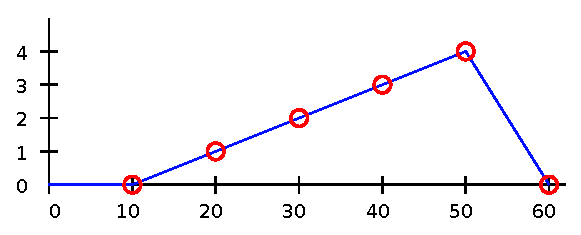
\includegraphics[width=\textwidth]{imatges/rrdtool/mostreig_regular.eps}
  \caption{Moviment d'un mòbil: perfil de velocitat en blau, punts de mostreig en vermell}
  \label{fig:rrdtool:mostreig_regular}
\end{figure}

En primer lloc, es crea una base de dades de nom \emph{velocitat.rrd} amb un temps de mostreig de 10 segons i un registre anomenat \emph{mps} que emmagatzema la velocitat del mòbil.
\begin{lstlisting}[style=sh]
export TZ=UTC
rrdtool create velocitat.rrd --start 1262304000 --step 10 \
        DS:mps:GAUGE:600:-U:U                              \ 
        RRA:AVERAGE:0.5:1:24                                                   
\end{lstlisting}


En segon lloc, s'actualitza la base de dades amb els valors $x=[0,1,2,3,4,0]$ que s'han mesurat als temps $t=[10,20,30,40,50,60]$.
\begin{lstlisting}[style=sh]
rrdtool update velocitat.rrd 1262304010:0 1262304020:1 1262304030:2 1262304040:3 1262304050:4 1262304060:0
\end{lstlisting}

Si es mostra el contingut de la base de dades, amb \verb+rrdtool dump+, es pot veure com els valors han entrat correctament:
\begin{lstlisting}
00:00:00 UTC  --> <row><v>NaN</v></row>
00:00:10 UTC  --> <row><v>0.0000000000e+00</v></row>
00:00:20 UTC  --> <row><v>1.0000000000e+00</v></row>
00:00:30 UTC  --> <row><v>2.0000000000e+00</v></row>
00:00:40 UTC  --> <row><v>3.0000000000e+00</v></row>
00:00:50 UTC  --> <row><v>4.0000000000e+00</v></row>
00:01:00 UTC  --> <row><v>0.0000000000e+00</v></row>
\end{lstlisting}


Finalment, es demana a RRDtool que faci un gràfic dels valors anteriors, el resultat es pot veure a la figura~\ref{fig:rrdtool:velocitat}:
\begin{lstlisting}[style=sh]
rrdtool graph velocitat.eps -a EPS --start 1262303999 --end 1262304060 DEF:vel=velocitat.rrd:mps:AVERAGE LINE1:vel#0000FF:"velocitat en m/s\l" -v "m/s" --x-grid SECOND:10:SECOND:10:SECOND:10:0:%X
\end{lstlisting}

\begin{figure}[htp]
  \centering
  \includegraphics[width=\textwidth]{imatges/rrdtool/velocitat.eps}
  \caption{Velocitats emmagatzemades a RRDtool d'un tipus Gauge}
  \label{fig:rrdtool:velocitat}
\end{figure}



D'aquest gràfic es desprèn com RRDtool interpreta les sèries temporals en sentit de passat. Els valors desats es representen constants en l'interval anterior al temps que els correspon. En l'exemple, a l'interval de temps (0,10] hi ha el valor 0, en l'interval (10,20] hi ha el valor 2, etc. En el temps 0, el valor és desconegut ja que no hi ha informació per l'interval anterior a zero.

Concloent, aquest és un exemple mostrejat de manera poc adequada  segons la idea de RRDtool. El mòbil de la figura~\ref{fig:rrdtool:mostreig_regular} té un perfil de velocitats mostrejat amb el valor instantani i aquest correspondria al mateix cas que mesurar una magnitud com la temperatura. Per mostrejar amb la idea de velocitat de RRDtool caldria que la velocitat fos constant; de fet, aleshores el perfil de velocitats original seria el de la figura~\ref{fig:rrdtool:velocitat}.

Si la velocitat no és constant, com és el cas de l'exemple, aleshores per complir amb la idea de RRDtool el valor mostrejat hauria d'informar de la velocitat en el darrer interval. Per exemple, amb la velocitat mitjana de cada interval ($x=[0,\ 0{,}5,\ 1{,}5,\ 2{,}5,\ 3{,}5 ,\ 2]$) ja s'aconsegueix una millor aproximació a la idea de RRDtool. Encara és més, en el concepte de RRDtool aquest exemple s'hauria de passar al domini de comptadors; és a dir mesurar l'espai recorregut en comptes de la velocitat. En els apartats següents es tractarà amb més detall els comptadors.


\subsection{Comptador monòton: \emph{Counter}}

Les dades de tipus Counter són dades provinents de comptadors. Aquestes dades no són velocitats i per tant cal aplicar transformació. 

Un comptador és un aparell de mesura que comença a zero i es va incrementant de manera contínua i monòtona en relació al paràmetre que està mesurant. A diferència d'una magnitud, un comptador no només indica el valor instantani de la variable sinó que informa dels valors des de l'última mesura. En anglès hi ha dues paraules que es tradueixen com a comptador: \emph{counter}, utilitzat en general, i \emph{meter}, utilitzat per exemple en energia elèctrica, en gas, en odometria, etc.

Per a transformar els valors d'un comptador a velocitat, a RRDtool se segueix el procediment següent.
En un moment determinat es pren el valor del comptador i al cap d'un temps definit es torna a consultar. Fent la diferència dels dos valors s'obté l'increment. Si a més es divideix per la diferència dels temps, el resultat és la mitjana del valor per unitat de temps; és a dir, una velocitat. A RRDtool el temps es mesura en segons, per tant les velocitats sempre es desen amb unitats de \emph{magnitud/s}. 
\begin{equation}\label{eq:rrdtool:rate}
c_2 \geq c_1 \longrightarrow\text{mitjana per }u.t. =\frac{c_2-c_1}{t_2-t_1}
\end{equation}
on $c_2$ i $t_2$ són el valor del comptador i el temps actual  i $c_1$ i $t_1$ són en el temps anterior.

RRDtool només emmagatzema velocitats. Per tant en les dades tipus comptador sempre calcula aquesta proporció mitjana del valor en cada període. Per exemple si el comptador mesura quilòmetres (km), el valor desat són velocitats (km/s).
Per aquesta mateixa raó, el primer valor que es desa a la base de dades no es pot calcular, ja que l'anterior no existeix, i es considera desconegut.

Els comptadors no poden decréixer però tenen un valor màxim que quan hi arriben tornen a començar des de zero. És a dir, els comptadors es poden desbordar (\emph{counter wraps}). RRDtool té en compte aquest cas i calcula l'increment real que s'ha produït. 
\begin{equation}\label{eq:rrdtool:wrap}
c_2 < c_1 \longrightarrow \text{mitjana per }u.t. =\frac{(\text{fons d'escala} -c_1)+c_2}{t_2-t_1}
\end{equation}
on ara, a diferència de l'equació~\ref{eq:rrdtool:rate}, cal tenir en compte el fons d'escala del comptador. 

Ara bé, de moment RRDtool només reconeix comptadors de 32 o 64 bits, els quals tenen rangs hexadecimals de 0 a FFFFFFFF$_h$ i de 0 a FFFFFFFFFFFFFFFF$_h$ respectivament. Si el rang del comptador és diferent d'aquests dos, el valor calculat és erroni
\footnote{En comptes del tipus \emph{counter} es pot utilitzar el tipus \emph{derive} amb el límit de velocitat mínima a zero. Llavors no es calculen valors erronis en els desbordaments sinó que es consideren desconeguts. Sigui quina sigui la manera, RRDtool no sap tractar aquests comptadors de manera adequada.\label{peu:rrdtool:counter}}.

Alguns exemples de comptador són el comptaquilòmetres d'un cotxe, els bytes transferits d'un router, la quantitat de pàgines impreses, el nombre de visitants, etc.


\paragraph{Exemple} Ara en el mòbil anterior de la figura~\ref{fig:rrdtool:velocitat}, en comptes de mesurar la velocitat es mesura l'espai recorregut com es veu a la figura~\ref{fig:rrdtool:mostreig_comptador}, també cada 10 segons. 

\begin{figure}[htp]
  \centering
  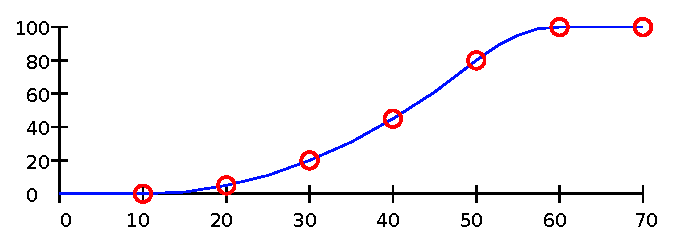
\includegraphics[width=\textwidth]{imatges/rrdtool/mostreig_comptador.eps}
  \caption{Moviment d'un mòbil: perfil d'espai recorregut en blau, punts de mesura en vermell}
  \label{fig:rrdtool:mostreig_comptador}
\end{figure}

En primer lloc, es crea una base de dades de nom \emph{comptador.rrd} amb un temps de mostreig de 10 segons i un registre anomenat \emph{mps} que emmagatzema la velocitat del mòbil però les dades d'entrada són l'espai recorregut.
\begin{lstlisting}[style=sh]
export TZ=UTC
rrdtool create comptador.rrd --start 1262304000 --step 10 \
        DS:mps:COUNTER:600:-U:U                           \ 
        RRA:AVERAGE:0.5:1:24                                                   
\end{lstlisting}

En segon lloc, s'actualitza la base de dades amb els valors $x=[0,5,20,45,80,100,100]$ que s'han mesurat als temps $t=[10,20,30,40,50,60,70]$ 

\begin{lstlisting}[style=sh]
rrdtool update comptador.rrd 1262304010:0 1262304020:5 1262304030:20 1262304040:45 1262304050:80 1262304060:100 1262304070:100
\end{lstlisting}

Si es mostra el contingut de la base de dades es pot veure com no hi ha els mateixos valors que s'han inserit; 
el gràfic de la figura~\ref{fig:rrdtool:comptador} que ha generat  RRDtool també corrobora aquestes dades:
\begin{lstlisting}
00:00:00 UTC  --> <row><v>NaN</v></row>
00:00:10 UTC  --> <row><v>NaN</v></row>
00:00:20 UTC  --> <row><v>5.0000000000e-01</v></row>
00:00:30 UTC  --> <row><v>1.5000000000e+00</v></row>
00:00:40 UTC  --> <row><v>2.5000000000e+00</v></row>
00:00:50 UTC  --> <row><v>3.5000000000e+00</v></row>
00:01:00 UTC  --> <row><v>2.0000000000e+00</v></row>
00:01:10 UTC  --> <row><v>0.0000000000e+00</v></row>
\end{lstlisting}

 
\begin{figure}[htp]
  \centering
  \includegraphics[width=\textwidth]{imatges/rrdtool/comptador.eps}
  \caption{Velocitats emmagatzemades a RRDtool d'un tipus Counter}
  \label{fig:rrdtool:comptador}
\end{figure}

En aquest gràfic, on les unitats són de metres per segon, es veu l'efecte de desar les dades en velocitat. Com que l'entrada de dades és de tipus comptador, RRDtool s'encarrega de transformar els valor a velocitat segons les equacions \ref{eq:rrdtool:rate} i \ref{eq:rrdtool:wrap} i també es compleix que el primer valor inserit s'emmagatzema com a desconegut ja que no es pot calcular. 

En referència a l'espai recorregut, es pot calcular multiplicant cada valor emmagatzemat pel temps de mostreig (10 segons). Aleshores s'obté 
$[u , 5 , 15 , 25 , 35 , 20 , 0]$
a on cada valor és l'increment d'espai recorregut en cada interval de temps corresponent; és a dir en els intervals
$[\ (0,10], (10,20], \ldots, (60,70]\ ]$.
 Per calcular l'espai recorregut total entre el temps 10 i el temps 70 s'ha de sumar aquests increments, aleshores s'obté el comptatge total de 100 metres que es correspon correctament amb el de la figura~\ref{fig:rrdtool:mostreig_comptador}.





\subsection{Comptador doble:  \emph{Derive}}

Les dades de tipus derive són de tipus comptador que tant pot incrementar com decrementar el valor; per això l'anomenem comptador doble. Aquestes dades no són velocitats i per tant cal aplicar transformació. 

La transformació a velocitat es calcula amb l'equació~\ref{eq:rrdtool:rate}, de la mateixa manera que els comptadors de tipus \emph{counter}. Però en els \emph{derive} no es té en compte el desbordament, sinó que un decrement del comptador es transforma a una velocitat negativa:  
$$
\text{mitjana per }u.t. =\frac{c_2-c_1}{t_2-t_1}
$$

Com que es desactiva el detector de desbordaments, el tipus \emph{derive} també s'utilitza per als \emph{counter} que no són ni de 32 ni de 64 bits. En aquests casos es configura el límit mínim de velocitat a zero i quan hi ha el desbordament\footnote{Això no es pot considerar una bona solució, vegeu nota~\ref{peu:rrdtool:counter}.} el valor transformat es considera desconegut, ja que la velocitat calculada és inferior al límit imposat de valor zero. 

Alguns exemples de comptador \emph{derive} són una bomba de cabal que pot bombejar o succionar, un comptador elèctric que mesura el total d'energia consumida menys la produïda, el balanç de població que emigra menys la que immigra, el saldo d'una llibreta que té ingressos i despeses, la quantitat de productes d'una màquina de \emph{vending}, etc. 


\paragraph{Exemple} Es mesura el saldo d'una llibreta d'estalvi que inicialment està a 0\euro, al cap de 10 segons rep un ingrés de 10\euro, al cap de 10 segons rep 20\euro\ i al cap de 10 segons té una despesa de 15\euro. 

Els valors que va prenent la llibreta (el comptador) es poden veure a la figura~\ref{fig:rrdtool:mostreig_derive}. Les mostres es prenen a l'instant abans que es faci l'operació d'ingrés o despesa; és a dir que la llibreta mostra el valor que ha tingut a l'interval anterior, la qual és la manera com s'entenen les sèries temporals a RRDtool. 

\begin{figure}[htp]
  \centering
  \includegraphics[width=\textwidth]{imatges/rrdtool/mostreig_derive.eps}
  \caption{Llibreta d'estalvi: valor del saldo en blau, punts de mesura en vermell}
  \label{fig:rrdtool:mostreig_derive}
\end{figure}

A més, RRDtool entén que les variables mesurades són contínues. Per tant amb les mesures fetes de la llibreta entén que el valor s'ha incrementat de manera contínua en tot l'interval. Això es pot observar a la línia discontínua de la figura~\ref{fig:rrdtool:mostreig_derive}, que és l'aproximació que fa RRDtool ja que només es guarda la velocitat mitjana a l'interval.

Es crea una base de dades de nom \emph{derive.rrd} amb un temps de mostreig de 10 segons i un registre anomenat \emph{eurps} que emmagatzema la velocitat del comptador (del saldo de la llibreta) a partir de les lectures del saldo. 

\begin{lstlisting}[style=sh]
export TZ=UTC
rrdtool create derive.rrd --start 1262304000 --step 10 \
        DS:eurps:DERIVE:600:-U:U                       \ 
        RRA:AVERAGE:0.5:1:24                                                   
\end{lstlisting}


S'actualitza la base de dades amb els valors $x=[0,0,10,30,15,15]$ que s'han mesurat als temps $t=[10,20,30,40,50,60]$ 

\begin{lstlisting}[style=sh]
rrdtool update derive.rrd 1262304010:0 1262304020:0 1262304030:10 1262304040:30 1262304050:15 1262304060:15
\end{lstlisting}

A continuació es mostren els valors emmagatzemats i a la figura~\ref{fig:rrdtool:derive} es mostra el gràfic que genera RRDtool:
\begin{lstlisting}
00:00:00 UTC  --> <row><v>NaN</v></row>
00:00:10 UTC  --> <row><v>NaN</v></row>
00:00:20 UTC  --> <row><v>0.0000000000e+00</v></row>
00:00:30 UTC  --> <row><v>1.0000000000e+00</v></row>
00:00:40 UTC  --> <row><v>2.0000000000e+00</v></row>
00:00:50 UTC  --> <row><v>-1.5000000000e+00</v></row>
00:01:00 UTC  --> <row><v>0.0000000000e+00</v></row>
\end{lstlisting}


\begin{figure}[htp]
  \centering
  \includegraphics[width=\textwidth]{imatges/rrdtool/derive.eps}
  \caption{Velocitats emmagatzemades a RRDtool d'un tipus Derive}
  \label{fig:rrdtool:derive}
\end{figure}

Aquest gràfic és com l'analitzat en l'exemple dels tipus \emph{counter} (figura~\ref{fig:rrdtool:comptador}), amb la diferència que ara en els \emph{derive} hi apareixen velocitats negatives. 
Com s'ha fet en els \emph{counter}, es pot calcular els increments de saldo de cada interval multiplicant les velocitats pel temps de mostreig. Aleshores els increments de saldo són $[u,0,10,20,-15,0]$ que sumats donen correctament els 15\euro\ de saldo final de la figura~\ref{fig:rrdtool:mostreig_derive}.


\subsection{Comptador relatiu: \emph{Absolute}}

Les dades de tipus Absolute són de tipus comptador d'increments; per això l'anomenen comptador relatiu. Aquestes dades no són velocitats i per tant cal aplicar transformació. 

Un comptador d'increments mesura directament la diferència des de l'última lectura, es pot veure com un comptador que es posa a zero a cada lectura. Per tant, per transformar les mesures a velocitat es divideix l'increment per la diferència de temps
$$
\text{mitjana per }u.t. =\frac{\Delta c}{t_2-t_1}
$$
on ara, a diferència de l'equació~\ref{eq:rrdtool:rate}, es mesura directament el comptatge ($\Delta c$) des de la mesura anterior.

Els increments mesurats poden ser positius o negatius; és a dir com en el cas \emph{derive} les velocitats resultants poden ser positives o negatives. Per tant, el tipus \emph{absolute} és el mateix que el \emph{derive} amb la diferència que el valor mesurat, el qual és el valor actual del comptador,  és un increment.

El primer valor que es desa a la base de dades ara es pot calcular, a diferència dels comptadors \emph{counter} i \emph{derive}. En aquest dos cal calcular l'increment de comptatge i en el primer valor és desconegut, ja que podria ser erroni suposar-lo com a zero. En el cas del comptador \emph{absolute} també cal indicar quin és el temps inicial, però aquest es considera que és el mateix que el d'inici de la base de dades.

Alguns exemples de comptador \emph{absolute} són els mateixos que en el \emph{derive} però mesurats de manera relativa: increments de bombeig o succió d'una bomba, la mesura de l'energia elèctrica en un cert temps, els increments de població degut a la migració, els registres a una llibreta, la venda o repostatge de productes, etc.

\paragraph{Exemple} Com en l'exemple del tipus \emph{derive} (figura~\ref{fig:rrdtool:mostreig_derive}), es mesura el saldo d'una llibreta d'estalvi. Ara, però, les mesures de comptador són les operacions d'ingrés o de despesa. El saldo pren els mateixos valors que en l'exemple anterior però ara les mesures són els increments, positius o negatius, que es poden veure a la figura~\ref{fig:rrdtool:mostreig_absolute}. 

\begin{figure}[htp]
  \centering
  \includegraphics[width=\textwidth]{imatges/rrdtool/mostreig_absolute.eps}
  \caption{Llibreta d'estalvi: increments de saldo en blau, punts de mesura en vermell, saldo en gris}
  \label{fig:rrdtool:mostreig_absolute}
\end{figure}

Les línies discontínues segueixen mostrant, com a la figura~\ref{fig:rrdtool:mostreig_derive}, l'aproximació que RRDtool fa del comptador com a variable contínua. 


Es crea una base de dades de nom \emph{absolute.rrd} amb un temps de mostreig de 10 segons i un registre anomenat \emph{eurps} que emmagatzema la velocitat del comptador (el saldo de la llibreta) a partir dels increments de saldo. 
\begin{lstlisting}[style=sh]
export TZ=UTC
rrdtool create absolute.rrd --start 1262304000 --step 10 \
        DS:eurps:ABSOLUTE:600:-U:U                        \ 
        RRA:AVERAGE:0.5:1:24                                                   
\end{lstlisting}


S'actualitza la base de dades amb els valors $x=[0,0,10,20,-15,0]$ que s'han mesurat als temps $t=[10,20,30,40,50,60]$ 
\begin{lstlisting}[style=sh]
rrdtool update absolute.rrd 1262304010:0 1262304020:0 1262304030:10 1262304040:20 1262304050:-15 1262304060:0
\end{lstlisting}

A continuació es mostren els valors emmagatzemats i a la figura~\ref{fig:rrdtool:absolute} es mostra el gràfic que genera RRDtool; és idèntic a la figura~\ref{fig:rrdtool:derive} però ara el primer valor és conegut.:
\begin{lstlisting}
00:00:00 UTC  --> <row><v>NaN</v></row>
00:00:10 UTC  --> <row><v>0.0000000000e+00</v></row>
00:00:20 UTC  --> <row><v>0.0000000000e+00</v></row>
00:00:30 UTC  --> <row><v>1.0000000000e+00</v></row>
00:00:40 UTC  --> <row><v>2.0000000000e+00</v></row>
00:00:50 UTC  --> <row><v>-1.5000000000e+00</v></row>
00:01:00 UTC  --> <row><v>0.0000000000e+00</v></row>
\end{lstlisting}


\begin{figure}[htp]
  \centering
  \includegraphics[width=\textwidth]{imatges/rrdtool/absolute.eps}
  \caption{Velocitats emmagatzemades a RRDtool d'un tipus Absolute}
  \label{fig:rrdtool:absolute}
\end{figure}

D'aquest gràfic, com en el casos \emph{derive} i \emph{counter}, es pot obtenir els increments de comptatge a cada interval si es multiplica cada valor pel temps de mostreig (10 segons). Aquests valors es podrien observar en un gràfic de barres, tot i que RRDtool només treballa amb variables velocitat contínues i per tant no pot mostrar exactament aquest gràfics de barres del comptador. A la figura~\ref{fig:rrdtool:comptador_barres} s'utilitza RRDtool perquè dibuixi els valors pintant l'àrea i multiplicant l'escala de l'eix Y per 10; perquè fos un gràfic de barres cal imaginar que a l'eix X hi ha les etiquetes corresponents als intervals: $(0,10], (10,20], \ldots, (50,60]$ i que cada un d'aquest intervals és una barra.

\begin{figure}[htp]
  \centering
  \includegraphics[width=\textwidth]{imatges/rrdtool/comptador_barres.eps}
  \caption{Gràfic de barres a RRDtool d'un comptador}
  \label{fig:rrdtool:comptador_barres}
\end{figure}

Ara bé, RRDtool sí que té funcions per tractar amb càlculs típics dels comptadors, per exemple calcular el total del comptador en un interval de temps donat. En aquest cas, el total del comptador des de l'inici fins a una data correspon al saldo de la llibreta en aquella data. A continuació es calcula el saldo des del temps 0 fins al temps 60, el qual correspon als 15\euro\ de la figura~\ref{fig:rrdtool:mostreig_absolute}.:
\begin{lstlisting}[style=sh]
rrdtool graphv absolute.eps -a EPS --start 1262303999 --end 1262304060 DEF:saldo=absolute.rrd:eurps:AVERAGE VDEF:tot=saldo,TOTAL PRINT:tot:%lf\EUR/s
\end{lstlisting}

\begin{lstlisting}
print[0] = "15.000000EUR/s"
\end{lstlisting}

\section[Normalització]{Normalització de l'interval}
\label{sec:rrdtool-etapes:normalitzacio}

RRDtool emmagatzema les dades a intervals regulars, és a dir en el temps de mostreig desitjat (anomenat \emph{step}). Com que a la pràctica és difícil complir-lo amb exactitud, cal modificar les dades perquè encaixin en aquest temps; és a dir s'ha de normalitzar l'interval de la sèrie temporal.

Per a modificar els valors de la sèrie temporal, en el context de velocitat vist a l'apartat anterior es pot plantejar una modificació de dades que tracti de mantenir l'àrea de sota la corba. La interpretació física és que es manté la quantitat total de magnitud.
Per exemple si les dades són velocitats lineals en m/s es pot entendre el problema com que es modifica la velocitat però es manté l'espai recorregut. O bé si les dades són comptadors, com que s'ha desat la velocitat s'entén que s'està mantenint la quantitat total.

Així doncs, el problema a resoldre és el següent. Donada una sèrie temporal acotada a un temps final $T_F$
$$%
S=\{\mathbf{X(t)}; t=t_0,t_1,t_2,\ldots,t_F\}
$$
que no té un període de mesura regular 
$$
t_{i+1}\neq t_{i} + T 
$$
es vol convertir a una sèrie temporal normalitzada amb interval regulars tal que ara $T$ correspongui al període de mostreig $t_m$:
$$%
S^N=\{\mathbf{X^N(t^N)}; t^N=t_0,t_1,t_2,\ldots,t_k\}
$$
$$
t^N_{k+1}= t^N_{k} + t_m 
$$
$$
t^N_k < T_F
$$
on $N$ indica que els valors i els temps ara contenen els valors normalitzats:
$$
\mathbf{X^N}= [x^N(t^N_0),x^N(t^N_1),\ldots,x^N(t^N_{T_i})]
$$

En resum, el vector de mesures té la forma 
$$
\mathbf{X(t)} = [x_0,x_1,\ldots,x_{F-1},x_F]
$$
i amb la mateixa mida el vector de temps de mesures
$$
\mathbf{t}=[t_0,t_1 \ldots, t_{T_f-1}, t_{T_f} ]
$$

Però el vector de valors normalitzats té una mida diferent 
$$
\mathbf{X^N(t^N)} = [x^N_0, x^N_1, \ldots,x^N_k ]
$$
on el vector de temps de mostreig normalitzats té la forma
$$
\mathbf{t^N}=[0,t_m, 2t_m,3t_m, \ldots kt_m ]
$$


A l'hora de convertir la sèrie temporal RRDtool utilitza el criteri de mantenir constant l'àrea sota la corba; a l'apartat~\ref{sec:rrdtool-etapes:gauge} s'ha vist com RRDtool representa les sèries temporals en velocitat i en passat. En els exemples d'aquest apartat, però, les mesures es feien en el temps de mostreig exacte, a continuació es mostrarà com RRDtool gestiona els casos en els que les mostres no coincideixen amb el temps de mostreig.

\subsection{Mostreig en temps real}

En un primer cas, la sèrie temporal original està mostrejada amb un únic valor a cada interval, tal com es faria en un sistema en temps real 
$$
\mathbf{X(t)}= [x(t_0)\ldots,x(t_{T_f-1}),x(t_{T_f})]
$$
$$
0< t_0 < t^N_1 < \cdots <   t^N_{i-1}<t_{T_f-1} < t^N_i < t_{T_f}
$$ 

En aquest cas, la sèrie temporal no té intervals regulars però sí que hi ha garantits uns terminis temporals en els que es disposa d'un valor i només hi ha un valor a cada interval:
$$
t_{i+1}\neq t_{i} + T 
$$
$$
t_{i+1} - t_{i} \leq t_m 
$$

A continuació es detalla com RRDtool normalitza la sèrie temporal en l'interval $[t^N_{i-1},t^N_i]$, es pot veure una interpretació gràfica a la figura~\ref{fig:rrdtool:normalitzacio}.

\begin{figure}[htp]
  \centering
  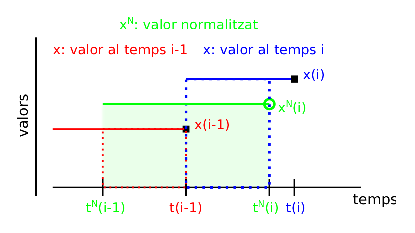
\includegraphics[width=\textwidth]{imatges/rrdtool/normalitzacio.eps}
  \caption{Normalització d'un interval}
  \label{fig:rrdtool:normalitzacio}
\end{figure}


Per una banda, es calcula l'àrea en l'interval seleccionat a partir dels valors mesurats
\[
A([t^N_{i-1},t^N_i]) = A([t^N_{i-1},t_{i-1}])+A([t_{i-1},t^N_i]) = ( t_{i-1} - t^N_{i-1})x_{i-1} + ( t^N_{i} - t_{i-1} )x_{i}
\]
i per altra banda, la normalització de l'interval s'expressa amb un valor de velocitat $X^N_i$ que es representa en el temps  $t^N_i$ degut a que RRDtool interpreta els valors en passat (constants en l'interval anterior)
\[
A^N = (  t^N_i - t^N_{i-1} )x^N_i  = t_m x^N_i
\]
Aleshores, s'igualen les dues expressions per tal que en normalitzar es conservi l'àrea en l'interval
\[
A^N=A([t^N_{i-1},t^N_i])
\]
d'on aïllant s'obté l'equació del valor normalitzat 
\begin{equation}\label{eq:rrdtool-etapes:normalitza}
x^N_i= \frac{(t_{i-1}-t^N_{i-1})x_{i-1} + (t^N_i-t_{i-1})x_i  }{t_m}
\end{equation}


El mateix es pot aplicar per tots els intervals de $\mathbf{X}$ per obtenir $\mathbf{X^N}$.



\paragraph{Exemple}


Agafem una nova base de dades velocitat.rrd i ara l'actualitzem amb el mateix perfil de velocitat de la figura~\ref{fig:rrdtool:mostreig_regular} però mostrejat de manera irregular com es veu a la figura~\ref{fig:rrdtool:mostreig_irregular}. A cada interval de mostreig hi segueix havent una mesura, i per tant compleixen el període de mostreig, però el temps de mostreig és irregular. Així ara els valors de velocitat mesurats són $x=[0, 0{,}5 , 1 , 2{,}8 , 3{,}2 , 2 , 0]$ en els temps $t=[10,15,20,38,42,55,65]$.


\begin{figure}[htp]
  \centering
  \includegraphics[width=\textwidth]{imatges/rrdtool/mostreig_irregular.eps}
  \caption{Mostreig en temps real: perfil de velocitat en blau, punts de mesura irregulars en vermell, període de mostreig de 10 segons}
  \label{fig:rrdtool:mostreig_irregular}
\end{figure}

S'insereixen els valors a la base de dades:
\begin{lstlisting}[style=sh]
rrdtool update velocitat.rrd 1262304010:0 1262304015:0.5 1262304020:1 1262304038:2.8 1262304042:3.2 1262304055:2 1262304065:0
\end{lstlisting}

A continuació es mostren els valors emmagatzemats i el gràfic que genera RRDtool (figura~\ref{fig:rrdtool:velocitat_irregular}):
\begin{lstlisting}
00:00:00 UTC  --> <row><v>NaN</v></row>
00:00:10 UTC  --> <row><v>0.0000000000e+00</v></row>
00:00:20 UTC  --> <row><v>7.5000000000e-01</v></row>
00:00:30 UTC  --> <row><v>2.8000000000e+00</v></row>
00:00:40 UTC  --> <row><v>2.8800000000e+00</v></row>
00:00:50 UTC  --> <row><v>2.2400000000e+00</v></row>
00:01:00 UTC  --> <row><v>1.0000000000e+00</v></row>
\end{lstlisting}


\begin{figure}[htp]
  \centering
  \includegraphics[width=\textwidth]{imatges/rrdtool/velocitat_irregular.eps}
  \caption{Valors emmagatzemats a RRDtool d'un mostreig en temps real}
  \label{fig:rrdtool:velocitat_irregular}
\end{figure}

Aplicant l'equació~\ref{eq:rrdtool-etapes:normalitza} als valors mesurats es pot comprovar que s'obtenen els valors normalitzats calculats per RRDtool 
$\mathbf{X^N}=[u , 0 , 0{,}75 , 2{,}8 , 2{,}88 , 2{,}24 , 1]$. 
Cal notar que a RRDtool el primer valor normalitzat, el qual correspon al temps $t^N_0$, és desconegut ja que no s'admeten insercions en el temps $t_0$.


\subsection{Ultramostreig}

En la normalització anterior de mostreig en temps real, en cada període de mostreig només hi havia una mesura. Ara bé, RRDtool permet que en cada interval hi hagi més d'una mesura i per tant hi pot haver més d'un valor a l'hora de normalitzar; anomenem aquest mostreig com ultramostreig (\emph{upsampling}), representat a la figura~\ref{fig:rrdtool-etapes:ultramostreig}.
$$
\mathbf{X(t)}= [x(t_0)\ldots,x(t_{T_f-k}),\cdots,x(t_{T_f-2}),x(t_{T_f-1}),x(t_{T_f})]
$$
$$
0< t_0 < t^N_1 < \cdots <   t^N_{i-1}<t_{T_f-k} <\cdots< t_{T_f-1} < t^N_i < t_{T_f}
$$

\begin{figure}[tbp]
  \centering
  \begin{tikzpicture}
    \begin{axis}[
        xlabel=temps ,
        ylabel= valor,
        xticklabels={0,$t_1^N$,$\ldots$,$t_{i-1}^N$,$t_i^N$},
        ]
    \addplot[ycomb,blue] coordinates {
        (0,10)
        (10,10)
        (20,10)
        (30,10)
        (40,10)
    }; 
 
    \addplot[only marks,mark=*,red] coordinates {
        (5,1)
        (32,2)
        (35,3)
        (38,4)
        (45,5)
    };

    \node[above] at (axis cs:5,1) {$t_0$};
    \node[below] at (axis cs:32,2) {$t_{T_f -k}$};
    \node[below] at (axis cs:35,3) {$\ldots$};
    \node[above] at (axis cs:38,4) {$t_{T_f -1}$};
    \node[above] at (axis cs:45,5) {$t_{T_f}$};

    \end{axis}
  \end{tikzpicture}
  \caption{Representació d'ultramostreig}
  \label{fig:rrdtool-etapes:ultramostreig}
\end{figure}

Aleshores, el valor normalitzat es calcula de la mateixa manera que a l'equació~\ref{eq:rrdtool-etapes:normalitza}, però ara el càlcul és una ponderació pel temps de tots els valors que cauen a dins de l'interval de normalització
\begin{equation}\label{eq:rrdtool:ultramostreig}
x^N_i = \frac{ (t_{T_f-k}-t^N_{i-1})x_{f-k} + \cdots + (t_{T_f-1}-t_{T_f-2})x_{f-1} + (t^N_i-t_{T_f-1})x_f }{t_m}
\end{equation}


Seguint aquesta equació de manera iterativa, es pot calcular el vector de valors normalitzats $\mathbf{X^N}$  per tots els $\mathbf{X(t)}$ amb l'algoritme següent:

\begin{lstlisting}[mathescape=true]  
Normalització d'una sèrie temporal amb ultramostreig 
a períodes de mostreig regulars 
INPUT: 
      vector de valors $\mathbf{X} = [x_0,x_1,\ldots,x_f]$ 
      vector de temps $\mathbf{t} = [t_0,t_1,\ldots,t_f]$
      període de mostreig regular  $t_m$
OUTPUT: 
      vector de valors normalitzats $\mathbf{X^N} = [x_0^N,x_1^N,\ldots,x_k^N]$

$x^N_0$ := unknown
$t^N_0$ := 0
$t^N_1$ := $t_0^N$ + $t_m$
i := 1

$A$ := $x_0t_0$   <-- àrea acumulada inicial 
k := 1

mentre k $\leq$ dim(x) fes

    si $t_k < t_i^N$ llavors
        $A$ := $A + x_k( t_k-t_{k-1}) $ <-- acumulació
        k := k+1
    sino 
        $x_i^N$ := $\dfrac{A + x_k( t_i^N-t_{k-1} )}{t_m}$

        $t_{i+1}^N$ := $t_i^N$ + $t_m$
        $A$ := $x_k*( t_k-t_i^N )$ <-- àrea acumulada inicial 
        k := k+1
        i := i+1
    fsi 

fmentre

\end{lstlisting}

\paragraph{Exemple}

Agafem una nova base de dades velocitat.rrd i ara l'actualitzem amb el mateix perfil de velocitat de la figura~\ref{fig:rrdtool:mostreig_regular} però amb més mostres en algun interval com es veu a la figura~\ref{fig:rrdtool:ultramostreig}. A cada interval de mostreig hi segueix havent com a mínim una mesura i compleixen el període de mostreig però en algun interval hi ha més d'una mostra. Així ara el valors de velocitat mesurats són $x=[0 , 0{,}5 , 0{,}8 , 1 , 2{,}8 , 3{,}2 , 3{,}5 , 3{,}8 , 2 , 0]$ en els temps $t=[10 , 15 , 18, 20, 38, 42, 45, 48, 55, 65]$.


\begin{figure}[htp]
  \centering
  \includegraphics[width=\textwidth]{imatges/rrdtool/sobremostreig.eps}
  \caption{Ultramostreig: perfil de velocitat en blau, punts de mesura (alguns ultramostrejats) en vermell, període de mostreig de 10 segons}
  \label{fig:rrdtool:ultramostreig}
\end{figure}

S'insereixen els valors a la base de dades:
\begin{lstlisting}[style=sh]
rrdtool update velocitat.rrd 1262304010:0 1262304015:0.5 1262304018:0.8 1262304020:1 1262304038:2.8 1262304042:3.2 1262304045:3.5 1262304048:3.8 1262304055:2 1262304065:0
\end{lstlisting}

A continuació es mostren els valors emmagatzemats i el gràfic que genera RRDtool (figura~\ref{fig:rrdtool:velocitat_ultramostrejada}):

\begin{lstlisting}
00:00:00 UTC  --> <row><v>NaN</v></row>
00:00:10 UTC  --> <row><v>0.0000000000e+00</v></row>
00:00:20 UTC  --> <row><v>6.9000000000e-01</v></row>
00:00:30 UTC  --> <row><v>2.8000000000e+00</v></row>
00:00:40 UTC  --> <row><v>2.8800000000e+00</v></row>
00:00:50 UTC  --> <row><v>3.2300000000e+00</v></row>
00:01:00 UTC  --> <row><v>1.0000000000e+00</v></row>
\end{lstlisting}


\begin{figure}[htp]
  \centering
  \includegraphics[width=\textwidth]{imatges/rrdtool/velocitat_sobremostrejada.eps}
  \caption{Valors emmagatzemats a RRDtool d'un ultramostreig}
  \label{fig:rrdtool:velocitat_ultramostrejada}
\end{figure}

Respecte a la figura~\ref{fig:rrdtool:velocitat_irregular} del cas de mostreig en temps real, ara només han canviat els valors dels intervals ultramostrejats mentre que els altres intervals continuen valent el mateix: $\mathbf{X^N}=[u , 0 , \underline{0{,}69} , 2{,}8 , 2{,}88 , \underline{2{,}24} , 1]$. Els valors que canvien són molt semblants als anteriors, però es pot dir que es té una millor aproximació a la velocitat real ja que en aquests intervals s'ha mostrejat més.

\subsection{Inframostreig}

Per altra banda, quan en un interval no hi ha cap mesura, és a dir que el temps de mostreig supera al període de mostreig, s'anomenem inframostreig (\emph{downsampling}).
$$
\mathbf{X(t)}= [x(t_0)\ldots,x(t_{T_f-1}),x(t_{T_f})]
$$
$$
t^N_{i-m-1} < t_{T_f-1} < t^N_{i-m} < \cdots < t^N_{i-1} < t^N_i < t_{T_f}
$$ 

\begin{figure}[tbp]
  \centering
  \begin{tikzpicture}
    \begin{axis}[
        width=10cm,scale only axis, height=5cm,
        xlabel=temps ,
        ylabel= valor,
        xticklabels={0,$t_1^N$,$\ldots$,$t_{i-m-1}^N$,$t_{i-m}^N$,$\ldots$,$t_{i-1}^N$,$t_i^N$},
        ]
    \addplot[ycomb,blue] coordinates {
        (0,10)
        (10,10)
        (20,10)
        (30,10)
        (40,10)
        (50,10)
        (60,10)
        (70,10)
    }; 
 
    \addplot[only marks,mark=*,red] coordinates {
        (5,1)
        (32,2)
        (35,3)
        (38,4)
        (75,5)
    };

    \node[above] at (axis cs:5,1) {$t_0$};
    \node[below] at (axis cs:32,2) {$t_{T_f -k}$};
    \node[below] at (axis cs:35,3) {$\ldots$};
    \node[above] at (axis cs:38,4) {$t_{T_f -1}$};
    \node[above] at (axis cs:75,5) {$t_{T_f}$};

    \end{axis}
  \end{tikzpicture}
  \caption{Representació d'inframostreig}
  \label{fig:rrdtool-etapes:inframostreig}
\end{figure}


Llavors per normalitzar amb inframostreig RRDtool utilitza el valor del següent interval. En aquest cas se suposa que les mesures no tenen termini, més endavant s'afegeix el problema del termini (vegeu apartat~\ref{sec:rrdtool-etapes:termini}).

És a dir, quan entre dues mesures hi ha més temps que el temps de mostreig llavors el valor de l'última mesura $\mathbf{x}(t_{T_f})$ s'expandeix enrere fins arribar a l'altra $\mathbf{x}(t_{T_f-1})$  i es calcula el valor normalitzat d'aquest gran interval. Si hi ha inframostreig però no hi ha ultramostreig
$$
t^N_{i-m-1} < t_{T_f-1} < t^N_{i-m} 
$$ 
el valor normalitzat és:
$$
x^N = \frac{ (t_{T_f-1}-t^N_{i-m-1})x_{f-1} + (t^N_i-t_{T_f-1})x_f }{t^N_i - t^N_{i-m-1}}
$$

Generalitzant, si alhora hi ha inframostreig i ultramostreig, representat a la figura~\ref{fig:rrdtool-etapes:inframostreig},
\[
t^N_{i-m-1} <  t_{T_f-k} <\cdots< t_{T_f-1}  < t^N_{i-m} 
\] 
el valor normalitzat es calcula de la mateixa manera que a l'equació~\ref{eq:rrdtool:ultramostreig}, però en l'interval $[t^N_{i-m-1},t^N_i]$:
\begin{equation}\label{eq:rrdtool:inframostreig}
x^N = \frac{ (t_{T_f-k}-t^N_{i-m-1})x_{f-k} + \cdots + (t_{T_f-1}-t_{T_f-2})x_{f-1} + (t^N_{i}-t_{T_f-1})x_f }{t^N_i - t^N_{i-m-1}}
\end{equation}

Finalment, aquest valor normalitzat per inframostreig, hi hagi ultramostreig o no, és utilitzat en tots els intervals afectats:
\[
x^N = x^N_{i-m} = \cdots = x^N_{i}
\]


Es modifica l'algoritme de càlcul iteratiu anterior segons aquest inframostreig:

\begin{lstlisting}[mathescape=true]
Normalització d'una sèrie temporal amb inframostreig
a períodes de mostreig regulars 
INPUT: 
      vector de valors $\mathbf{X} = [x_0,x_1,\ldots,x_f]$ 
      vector de temps $\mathbf{t} = [t_0,t_1,\ldots,t_f]$
      període de mostreig regular  $t_m$
OUTPUT: 
      vector de valors normalitzats $\mathbf{X^N} = [x_0^N,x_1^N,\ldots,x_k^N]$

$x_0^N$ := unknown
$t_0^N$ := 0
$t_1^N$ := $t_0^N$ + $t_m$
i := 1

$A$ := $x_0t_0$
k := 1

mentre k $\leq$ dim(x) fes
    si $t_k < t_i^N$ llavors
        $A$ := $A + x_k( t_k-t_{k-1} )$
        k := k+1
    sino 
        $N_{inf}$ := $(t_k-t_i^N)$ div $t_m$ <-- n. d'intervals amb inframostreig

        $x_i^N$ := $\dfrac{A + x_k( t_i^N-t_{k-1} ) + x_k \cdot N_{inf} \cdot t_m}{t_m  (1+N_{inf})}$

        mateix valor per cada interval amb inframostreig
        $x_{i+N_{inf}}^N$ := $\,\cdots\,$ := $x_{i+1}^N$ := $x_i^N$
        $t_{i+1}^N$ := $t_i^N + (N_{inf}+1) t_m$
        i := i + ($N_{inf}$+1)
                
        $A$ := $x_k( t_k-t_{i-1}^N )$
        k := k+1
    fsi 
fmentre
\end{lstlisting}

\paragraph{Exemple}

Agafem una nova base de dades velocitat.rrd i ara l'actualitzem amb el mateix perfil de velocitat de la figura~\ref{fig:rrdtool:mostreig_regular} però en algun interval no hi ha mostres, com es veu a la figura~\ref{fig:rrdtool:inframostreig}. És important ressaltar que aquests intervals no compleixen el període de mostreig
 Així ara el valors de velocitat mesurats són $x=[0, 0{,}5 , 2{,}5 , 3{,}8 , 2 , 0]$ en els temps $t=[10, 15, 35, 48, 55, 65]$.

\begin{figure}[htp]
  \centering
  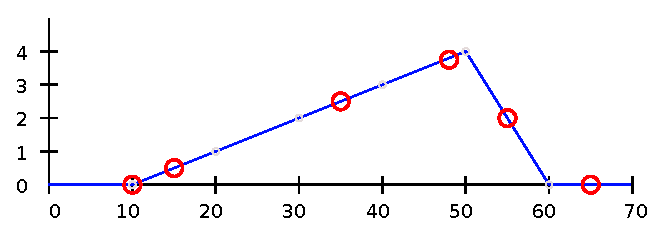
\includegraphics[width=\textwidth]{imatges/rrdtool/inframostreig.eps}
  \caption{Inframostreig: perfil de velocitat en blau, punts de mesura (alguns inframostrejats) en vermell, període de mostreig de 10 segons}
  \label{fig:rrdtool:inframostreig}
\end{figure}



S'insereixen els valors a la base de dades:
\begin{lstlisting}[style=sh]
rrdtool update velocitat.rrd 1262304010:0 1262304015:0.5 1262304035:2.5 1262304048:3.8 1262304055:2 1262304065:0
\end{lstlisting}

A continuació es mostren els valors emmagatzemats i el gràfic que genera RRDtool (figura~\ref{fig:rrdtool:velocitat_inframostrejada}):
\begin{lstlisting}
00:00:00 UTC  --> <row><v>NaN</v></row>
00:00:10 UTC  --> <row><v>0.0000000000e+00</v></row>
00:00:20 UTC  --> <row><v>2.0000000000e+00</v></row>
00:00:30 UTC  --> <row><v>2.0000000000e+00</v></row>
00:00:40 UTC  --> <row><v>3.1500000000e+00</v></row>
00:00:50 UTC  --> <row><v>3.4400000000e+00</v></row>
00:01:00 UTC  --> <row><v>1.0000000000e+00</v></row>
\end{lstlisting}


\begin{figure}[htp]
  \centering
  \includegraphics[width=\textwidth]{imatges/rrdtool/velocitat_inframostrejada.eps}
  \caption{Valors emmagatzemats a RRDtool d'un inframostreig}
  \label{fig:rrdtool:velocitat_inframostrejada}
\end{figure}


Respecte a la figura~\ref{fig:rrdtool:velocitat_irregular} del cas de mostreig en temps real, aquest gràfic només es diferencia en els intervals inframostrejats.
Ara els intervals afectats per l'inframostreig $(10,20]$ i $(20,30]$ tenen el mateix valor de 2, el qual resulta d'aplicar l'equació~\ref{eq:rrdtool:inframostreig}:  
$
x_{20}^N = x_{30}^N  = 
\frac{ (15-10) 0{,}5 + (30-15) 2{,}5 }{30 - 10}
= 2
$.
En aquests dos intervals hi ha una pitjor aproximació a la velocitat real ja que s'ha mostrejat molt poc.



\subsection{Tractament de dades desconegudes}

En les seccions anteriors, les mesures de les sèries temporals sempre tenen un valor numèric. En concret són números reals ($\mathbb{R}$), els quals es representen informàticament amb el format numèric de precisió doble seguint l'estàndard IEEE 754,~\cite{wiki:ieee754}.
 
Però les mesures, a més a més de tenir un valor, també poden ser desconegudes (\emph{unknown data}); és a dir, que no existeixin o que s'ignorin (es descartin).  Aquests valors desconeguts també estan contemplats a l'estàndard IEEE 754 i es representen  amb el valor numèric especial NaN (\emph{Not a Number}). 

L'algoritme de normalització d'intervals ha de saber manipular les mostres amb mesures desconegudes. En el cas de RRDtool, les dades desconegudes poden venir per tres vies:

\begin{itemize}
\item la mesura no existeix,
\item el temps de mesura ha superat el termini o
\item el valor de mesura està fora dels límits.
\end{itemize}

A continuació es detallen aquestes tres vies i al final es modifica l'algoritme de normalització en concordança amb el tractament d'aquestes dades desconegudes.

\subsubsection{Mesura inexistent}

Una mesura no existeix quan no s'ha pogut establir contacte amb el sensor o quan aquest retorna valors que no són númerics. Quan una mesura no existeix, es considera desconeguda i s'insereix a la base de dades amb el valor 'U' (\emph{unknown}) tot i que queda representat amb el valor NaN segons l'estàndard IEEE 754. 


Les mesures també es desconeixen quan s'inicialitza la base de dades. A l'inici d'una base de dades RRDtool es creen tots els registres fins al temps actual però aquestes mesures no han existit mai; per tant prenen 'desconegut' com a valor.


\paragraph{Exemple} S'insereix una dada amb valor conegut i l'altra amb valor desconegut

\begin{lstlisting}[style=sh]
rrdtool update velocitat.rrd 1262304010:1 1262304020:U 
\end{lstlisting}

\begin{lstlisting}
23:59:30 UTC  --> <row><v>NaN</v></row>
23:59:40 UTC  --> <row><v>NaN</v></row>
23:59:50 UTC  --> <row><v>NaN</v></row>
00:00:00 UTC  --> <row><v>NaN</v></row>
00:00:10 UTC  --> <row><v>1.0000000000e+00</v></row>
00:00:20 UTC  --> <row><v>NaN</v></row>
\end{lstlisting}

Per una banda, tots els valors anteriors al temps 0 (aquest inclòs) són desconeguts perquè no es coneix res abans que s'inicialitzi la base de dades. Per altra banda, s'ha inserit un valor numèric en el temps 10 i el valor 'desconegut' en el temps 20.



\subsubsection{Temps de termini}
\label{sec:rrdtool-etapes:termini}

El temps de termini, el qual RRDtool anomena \emph{heartbeat} ($t_h$), és el temps màxim que s'admet entre dues mesures. La mesura actual s'ignora si ha passat més temps que el termini des de la mesura anterior. 
$$
t_i - t_{i-1} > t_h \longrightarrow   x(t_i) = unknown 
$$
 
A RRDtool el termini pot ser més gran, igual o més petit que el temps de mostreig. És a dir, que el termini no només afecta en els casos d'inframosteig sinó que també al casos d'ultramostreig.


Cal no confondre el termini de RRDtool (\emph{heartbeat})  amb el termini utilitzat pels sistems de temps real (\emph{deadline}). El \emph{heartbeat} es mesura entre mostres amb l'objectiu de tenir dades 'fresques' i en canvi el \emph{deadline} es mesura a partir del temps d'activació amb l'objectiu de complir temps de càlcul. En el cas de tasques periòdiques, com és el cas del temps de mostreig a RRDtool, en temps real no té sentit parlar de terminis més grans que el període de mostreig, en canvi en els RRDtool ja s'ha vist que poden tractar aquestes situacions, anomenades inframostreig.


A continuació s'estudien  quatre casos diferents segons els valors que pot adoptar el temps de termini respecte del temps de mostreig. Els quatre casos es poden veure a l'eix vertical de la figura~\ref{fig:rrdtool:terminis} representant el termini amb $t_h$, el període de mostreig amb $t_m$ i exemples de temps de mesura amb una circumferència vermella a l'eix horitzontal. 

\begin{figure}[htp]
  \centering
  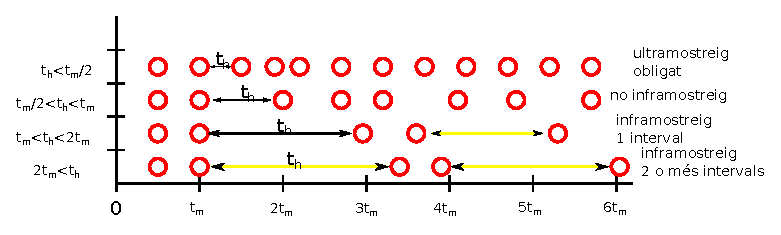
\includegraphics[width=\textwidth]{imatges/rrdtool/terminis.eps}
  \caption{Comparació de mostrejos amb terminis $t_h$ diferents pel mateix període de mostreig $t_m$, punts de mesura en vermell i intervals inframostrejats en groc}
  \label{fig:rrdtool:terminis}
\end{figure}

Primer de tot, del concepte de RRDtool es desprèn que en qualsevol cas sempre hi pot haver ultramostreig. Això és degut a que els terminis són els temps màxims entre mesures però no s'especifica un temps mínim. Aquestes situacions es poden veure a la figura~\ref{fig:rrdtool:terminis}: a l'eix horitzontal hi ha marcats els temps de mostreig exactes però el temps de mesura pot prendre qualsevol valor mentre sigui inferior al termini prefixat.


Un termini més gran que el temps de mostreig  ($t_h>t_m$) indica que s'accepten els casos d'inframostreig i el temps del termini limita el temps durant el qual es permet no disposar de mesures. A més, si el termini és més petit que el doble del temps de mostreig ($t_m<t_h<2t_m$), com a màxim només hi pot haver un interval amb inframostreig. Però si el termini supera el doble del temps de mostreig, llavors l'inframostreig es pot donar en dos intervals, en tres intervals si és el triple, etc.

Un termini més petit que el temps de mostreig ($t_h<t_m$) indica que no es vol inframostreig; és a dir que en cada interval com a mínim hi ha d'haver una mostra. Però, al mateix temps, un termini més petit que el temps de mostreig fa que a la llarga s'obligui a ultramostrejos en alguns intervals. Encara més, si el termini és inferior a la meitat del temps de mostreig, llavors hi ha d'haver ultramostreig en tots els intervals.

Normalment, en els usos de RRDtool, el valor del termini s'assigna a un valor més gran que el doble del temps de mostreig ($t_h>2t_m$) per tal de poder tenir folgança en les mesures. Cal observar que el cas del mostreig únic es representa amb el termini doblant el temps de mostreig ($t_h=2t_m$); això permet que la mesura següent se situi en qualsevol temps de l'interval de mostreig següent.

El cas del mostreig únic és comparable als sistemes en temps real. En els sistemes en temps real el temps entre mostres com a màxim pot doblar el temps de mostreig, mentre es compleixi que en cada interval de mostreig hi ha una mostra. En el cas de RRDtool, quan $t_h=2t_m$, hi pot haver inframostreig i per tant es pot no complir el temps real requerit pel mostreig únic. 
En conclusió, el temps de termini a RRDtool només s'utilitza per avaluar si les dades són 'fresques', la responsabilitat de les mesures i del temps real recau a la part d'adquisició de dades dels sistemes de monitoratge. 

A RRD el termini es defineix a l'hora de crear una base de dades però es pot tornar a configurar. Cada variable mesurada (cada registre) té el seu termini.


\paragraph{Exemple} Ara es crea la base de dades velocitat.rrd amb un temps de mostreig de 10 segons i un termini de 6 segons.

\begin{lstlisting}[style=sh]
rrdtool create velocitat.rrd --start 1262304000 --step 10 \
        DS:mps:GAUGE:6:-U:U                             \
        RRA:AVERAGE:0.5:1:24                                 
\end{lstlisting}

S'actualitza la base de dades amb els valors $x=[1,1,1]$ en els temps $t=[6,10,20]$.

\begin{lstlisting}[style=sh]
rrdtool update velocitat.rrd 1262304006:1 1262304010:1 1262304020:1 
\end{lstlisting}

A continuació es mostren els valors emmagatzemats:
\begin{lstlisting}
00:00:00 UTC  --> <row><v>NaN</v></row>
00:00:10 UTC  --> <row><v>1.0000000000e+00</v></row>
00:00:20 UTC  --> <row><v>NaN</v></row>
\end{lstlisting}

Les mesures implicades en el primer interval [0,10] han complert els terminis ja que el temps entre mesures és igual o inferior a 6 segons. Però en el segon interval [10,20], l'última mesura dista 10 segons respecte de l'anterior i per tant s'ignora i es considera desconeguda. 


\subsubsection{Límits}

Una altra comprovació que es fa a les mesures és si estan dins d'un rang. A RRDtool es comprova que el valor mesurat és més gran que un límit inferior i que és més petit que un límit superior. Si la mesura està fora de rang, s'ignora i es considera desconeguda.
$$
x(t_i) > L_{\max}  \longrightarrow   x(t_i) = unknown 
$$
$$
x(t_i) < L_{\min} \longrightarrow   x(t_i) = unknown 
$$

El límits sempre es calculen a les mesures un cop ja han passat l'etapa de transformació a velocitat. En el cas dels comptadors es comprova que la velocitat calculada estigui dins del rang però no es comprova la magnitud comptada, és a dir el valor que realment s'ha mesurat.

A RRDtool els límits es defineixen a l'hora de crear una base de dades però es poden tornar a configurar. Cada variable mesurada, això és cada registre, té el seus límits. Si no es vol comprovar el rang de les mesures, els límits es poden configurar amb el valor desconegut (\emph{U}) per tal que no es tinguin en compte. 


\paragraph{Exemple} Ara es crea la base de dades velocitat.rrd amb un límit inferior de 0 i un límit superior desconegut.

\begin{lstlisting}[style=sh]
rrdtool create velocitat.rrd --start 1262304000 --step 10 \
        DS:mps:GAUGE:600:0:U                             \
        RRA:AVERAGE:0.5:1:24                                 
\end{lstlisting}

Ara s'actualitza la base de dades amb els valors $x=[0,1000,-1]$ en els temps $t=[10,20,30]$.

\begin{lstlisting}[style=sh]
rrdtool update velocitat.rrd 1262304006:1 1262304010:1 1262304020:1 
\end{lstlisting}

A continuació es mostren els valors emmagatzemats:
\begin{lstlisting}
00:00:00 UTC  --> <row><v>NaN</v></row>
00:00:10 UTC  --> <row><v>0.0000000000e+00</v></row>
00:00:20 UTC  --> <row><v>1.0000000000e+03</v></row>
00:00:30 UTC  --> <row><v>NaN</v></row>
\end{lstlisting}

No hi ha límit superior però sí que n'hi ha d'inferior. En el temps 30 el valor és més petit que el límit i per tant s'ignora la mesura i es considera desconeguda.


\subsubsection{Càlcul amb dades desconegudes}

Fins ara s'ha vist les tres vies per on es poden obtenir dades desconegudes en la normalització d'intervals. Cal notar que les tres vies només serveixen per considerar si una mesura és desconeguda o no, però una mesura desconeguda no és suficient per considerar tot l'interval normalitzat desconegut.

A RRDtool, l'interval es considera desconegut\footnote{A l'etapa de normalització d'interval no es pot triar la quantitat de desconeguts que són acceptables, ni fins i tot poder decidir si un valor desconegut ja fa calcular tot l'interval com desconegut. A l'etapa de consolidació sí que és possible (v.\ secció~\ref{rrdtool:consolidacio:unknown}).}
quan el temps de mesures desconegudes ($T_u$)  és superior a la meitat del període de mostreig.
$$
T_u = \sum_{\forall x_f = unknown} ( t_f-t_{f-1} ) \quad
$$
$$
\text{si } T_u > t_m/2  \longrightarrow   x^N_{t^N_i} = unknown 
$$
sent $T_u$ el temps total que en un interval els valors $\mathbf{X}$ prenen valor desconegut.

En cas contrari es calcula l'interval amb els valors coneguts. És a dir, l'algoritme de normalització d'intervals ha de saber manipular les mostres amb mesures desconegudes. 
Per normalitzar, les dades desconegudes es considera que valen la mitjana de l'interval ($x_i^N=x_u$) .  D'aquesta manera no afecta a la velocitat mitjana de l'interval. Tot seguit es demostra.

\begin{figure}[tbp]
  \centering
  \begin{tikzpicture}
    \begin{axis}[
        width=10cm,scale only axis, height=5cm,
        xlabel=temps ,
        ylabel= valor,
        xticklabels={$\ldots$,,$t_{i-1}^N$,,$t_i^N$},
        ]
    \addplot[ycomb,blue] coordinates {
        (20,10)
        (30,10)
        (40,10)
    }; 
    \addlegendentry{}

    \addplot[ybar interval,yellow,fill=yellow!20!white] coordinates{
        (30,0)
        (30,10)
        (32,10)
        (32,0)
    };
    \addlegendentry{$t_a$}

   \addplot[ybar interval,purple,fill=purple!20!white] coordinates{
        (32,0)
        (32,10)
        (35,10)
        (35,0)
    };
    \addlegendentry{$t_{k-2}$}

    \addplot[ybar interval,orange,fill=orange!20!white] coordinates{
        (35,0)
        (35,10)
        (38,10)
        (38,0)
    };
    \addlegendentry{$t_0$}

    \addplot[ybar interval,green,fill=green!20!white] coordinates{
        (38,0)
        (38,10)
        (40,10)
        (40,0)
    };
    \addlegendentry{$t_b$}
 

 
    \addplot[only marks,mark=*,red] coordinates {
        (32,2)
        (35,3)
        (38,4)
        (45,2)
    };

    \node[below] at (axis cs:32,2) {$t_{T_f -k}$};
    \node[below] at (axis cs:35,3) {$\ldots$};
    \node[above] at (axis cs:38,4) {$t_{T_f -1}$};
    \node[above] at (axis cs:45,2) {$t_{T_f}$};



    \end{axis}
  \end{tikzpicture}
  \caption{Representació d'ultramostreig simplificada}
  \label{fig:rrdtool-etapes:desconeguts}
\end{figure}


Per una banda, la mitjana de l'interval sense tenir en compte els valors desconeguts es calcula utilitzant l'equació~\eqref{eq:rrdtool:ultramostreig} només en els valors coneguts. Per facilitar la comprensió, es reescriu l'equació utilitzant $t_a$, $t_b$ i $t_j$, representats a la figura~\ref{fig:rrdtool-etapes:desconeguts}:
$$%
t_a =t_{T_f-k}-t^N_{i-1} \quad\text{ i }\quad t_b = t^N_i-t_{T_f-1}
$$
$$
t_j =t_{T_f-1-j}-t_{T_f-2-j} \quad\forall j=[0,k-2]
$$
\begin{equation}\label{eq:rrdtool:normalitzacio}
x^N_i = \frac{t_ax_a+\sum\limits_{j=0}^{k-2} (t_jx_j)+t_bx_b}{t_a+\sum\limits_{j=0}^{k-2} (t_j)+t_b}
\end{equation}
Per altra banda, l'equació tenint en compte els valors desconeguts ($x_u$) és
\begin{equation}\label{eq:rrdtool:normalitzacio-desconegut}
x^N_i = \frac{t_ax_a+\sum\limits_0^{k-2} (t_jx_j)+t_bx_b+T_ux_u}{t_a+\sum\limits_0^{k-2} (t_j)+t_b+T_u}
\end{equation}
Substituint \eqref{eq:rrdtool:normalitzacio} a \eqref{eq:rrdtool:normalitzacio-desconegut} 
\[
x^N_i = \frac{ x_i^N(t_a+\sum\limits_0^{k-2} (t_j)+t_b)+T_ux_u}{t_a+\sum\limits_0^{k-2} (t_j)+t_b+T_u}
\]
operant amb aquesta expressió
\begin{align*}
 x^N_i - \frac{ x_i^N(t_a+\sum\limits_0^{k-2} (t_j)+t_b)+T_ux_u}{t_a+\sum\limits_0^{k-2} (t_j)+t_b+T_u} &= 0\\
 \frac{x^N_i(t_a+\sum\limits_0^{k-2} (t_j)+t_b+T_u) -  x_i^N(t_a+\sum\limits_0^{k-2} (t_j)+t_b)-T_ux_u}{t_a+\sum\limits_0^{k-2} (t_j)+t_b+T_u} &= 0\\
\frac{T_ux_i^N+T_ux_u}{t_a+\sum\limits_0^{k-2} (t_j)-t_b+T_u} &= 0
\end{align*}
Aleshores
\[
x_i^N = x_u
\]


Per tant si els valors desconeguts valen el mateix que la mitjana ($x_u=x^N_i$), aquesta mitjana es pot calcular senser tenir-los en compte com a l'equació~\ref{eq:rrdtool:normalitzacio}. En aquesta equació el temps de l'interval queda reduït, ja que el temps total de l'interval equival al temps de mostreig
$$
t_m= t_a+\sum\limits_0^{k-2} (t_j)+t_b+T_u
$$
i per tant es pot reexpressar a l'eq.~\ref{eq:rrdtool:normalitzacio} com el temps de mostreig descomptant-hi els temps en valors desconeguts
$$
t_a+\sum\limits_0^{k-2} (t_j)+t_b = t_m -T_u
$$

En resum, la normalització de l'interval es pot calcular amb l'àrea acumulada dels valors sense comptar-hi els desconeguts i al final dividida entre el temps de mostreig descomptant-hi els temps en valors desconeguts
$$
x^N_i = \frac{t_ax_a+\sum\limits_0^{k-2} (t_jx_j)+t_bx_b}{t_m - T_u}
\quad\forall\ x(t)\neq unknown
$$


Com que es dóna un valor al desconegut, això fa que la magnitud comptada augmenti. És a dir, s'està suposant que el comptador ha seguit mesurant a una velocitat semblant a les altres de l'interval.

Aquest augment s'observa seguint l'equació $e=x(t)$
$$
e_{mesurat} = x_at_a+\sum\limits_0^{k-2} (x_jt_j)+x_bt_b
$$
$$
e_{emmagatzemat} = x_at_a+\sum\limits_0^{k-2} (x_jt_j)+x_bt_b+x^N_iT_u
$$



% Atenció: sembla que hi ha un bug

% Heartbeat=600. Mentre que 
% rrdtool updatev consolida.rrd 1262304015:1 1262304030:U dóna 1(?),1(no) updatev consolida.rrd 1262304015:1 1262304029:U 1262304030:U dóna 1(bé),U(bé)

% però si Heartbeat=12 dóna U,U


% Un altre bug. Heartbeat=3 rrdtool updatev consolida.rrd 1262304013:1 1262304016:1 1262304019:1 1262304022:1 dóna 1(bé). rrdtool updatev consolida.rrd 1262304013:1 1262304017:1 1262304020:1 dóna 1(bé). però rdtool updatev consolida.rrd 1262304013:1 1262304016:1 1262304020:1 dóna U(no)

% %http://www.vandenbogaerdt.nl/rrdtool/total.php
% %http://www.mrtg.org/rrdtool/doc/rrdcreate.en.html



\subsection{Algoritme de normalització}
Ara es modifica l'algoritme tenint compte les dades desconegudes i també els ultramostrejos i inframostrejos dels intervals. Aquest és l'algoritme complet de normalització d'intervals.



\begin{lstlisting}[mathescape=true]
Normalització d'una sèrie temporal
a períodes de mostreig regulars 
INPUT: 
      vector de valors $\mathbf{X} = [x_0,x_1,\ldots,x_f]$ 
      vector de temps $\mathbf{T} = [t_0,t_1,\ldots,t_f]$
      període de mostreig regular  $t_m$
      termini $H$
      llindars màxim $X^{MAX}$ i mínim $X^{MIN}$
OUTPUT: 
      vector de valors normalitzats $\mathbf{X^N} = [x_0^N,x_1^N,\ldots,x_k^N]$

$x_0^N$ := unknown <-- primer valor normalitzat desconegut
$t^N$ := $t_m$ <-- següent interval de normalització
i := 1

$A$ := 0 <--- àrea acumulada
$t_{ant}$ := 0 <-- temps de la mostra anterior
$T_u$ := 0 <-- temps en valor desconegut

per cada parella $(x,t)$ en $\mathbf{X}$ i $\mathbf{T}$ fes:

    avalua termini i llindar:
    si $t-t_{ant}$ > $H$ o no $X^{MIN}$ $\leq$ x $\leq$ $X^{MAX}$ llavors x:= unknown fsi

    si $t < t^N$ llavors
        si x = unknown llavors
            $T_u$ := $T_u + t -t_{ant}$ <-- acumula temps desconegut
        sino
            $A$ := $A + x( t-t_{ant} )$ <-- acumula valor
        fsi

    sino  <-- càlcul d'un valor normalitzat

        $N_{inf}$ := $(t-t^N)$ div $t_m$ <-- n. d'intervals amb inframostreig

        si x = unknown llavors
            $T_u$ := $T_u+t^N -t_{ant} +N_{inf}\cdot t_m$ <-- acumula temps desconegut
        sino
            $x_i^N$ := $A + x( t^N-t_{ant} ) + x \cdot N_{inf} \cdot t_m$ <-- acumula valor
        fsi

        si $T_u > \frac{(1+N_{inf})t_m}{2}$ llavors
            $x_i^N$ := unknown <--  normalitza desconegut
        sino
            $x_i^N$ := $\dfrac{A}{t_m (1+N_{inf})-T_u}$ <--  normalitza valor
        fsi

        mateix valor per cada interval amb inframostreig
        $x_{i+N_{inf}}^N$ := $\,\cdots\,$ := $x_{i+1}^N$ := $x_i^N$
                
        si x = unknown llavors <-- acumula desconegut, reset àrea 
            $T_u$ := $t-t_{ant}$
            $A$ := 0
        sino <-- acumula àrea, reset desconeguts
            $T_u$ := 0
            $A$ := $x( t-t^N )$
        fsi

        $t^N$ := $t^N + (N_{inf}+1) t_m$ <-- següent interval de normalització
        i := i + ($N_{inf}$+1)

    fsi 

    $t_{ant}$ := $t$

repeteix
\end{lstlisting}




\section[Consolidació]{Consolidació d'intervals}

Un cop s'ha normalitzat l'interval, a la base de dades hi ha els valors amb temps de mostreig regular (\emph{step}). Aquest valors ja normalitzats a RRDtool s'anomenen \emph{Primary Data Points} (PDP). 

Però aquest interval de mostreig inicial no es pot mantenir durant gaire temps ja que cada cop és més difícil gestionar la quantitat de dades. Per afitar la quantitat de dades emmagatzemades, RRDtool desa les dades en diferents resolucions temporals. 

És a dir, cal consolidar l'interval normalitzat inicial a altres temps de mostreig desitjats. A partir dels PDP es tornen a mostrejar (\emph{resampling}) nous intervals amb menys resolució. 

A RRDtool, aquest valors nous consolidats s'anomenen \emph{Consolidated Data Points} (CDP) i cada resolució s'emmagatzema en les taules anomenades \emph{Round Robin Archive} (RRA).
Cada CDP es calcula a partir de $n$ PDP i cada RRA defineix aquest $n$ necessari, el qual a RRDtool s'anomena \emph{step} però que cal no confondre'l amb l'\emph{step} de normalització d'interval. Es poden distingir com a \emph{step de CDP} i \emph{step de PDP}, respectivament.


En aquest càlcul pot interessar conservar diferent informació de les variables mesurades. El canvi de resolució implica una pèrdua de precisió i informació, cal trobar un càlcul que mantingui les propietats que interessin de les dades

Per un RRA que aplica una funció $f$ de consolidació a $n$ PDP (valors normalitzats $V^N$) per obtenir un CDP:
$$
CDP_i = f(x^N_{i-n},\ldots,x^N_i) \qquad i \in \{ n,2n,3n\ldots \}
$$

És a dir que la resolució dels CDP sempre és múltiple del temps de mostreig base dels PDP. 
Actualment RRDTool permet calcular quatre funcions de consolidació: 

\begin{itemize}
\item mitjana (AVERAGE)
\item màxim (MAX)
\item mínim (MIN)
\item últim (LAST)
\end{itemize}

% Aquestes funcions tenen la particularitat que es poden calcular de manera incremental.
% $$
% CDP_i =   f(f( \ldots( f(f(unknown,x^N_{i-n}), x^N_{i-n+1}),\ldots ), x^N_{i-1}) ,x^N_i )  \qquad i \in \{ n,2n,3n\ldots \}
% $$


Calcular la mitjana és equivalent al que es fa a l'etapa de normalització de l'interval. En aquell cas cal fer una mitjana ponderada per la durada de la mesura però ara els intervals són iguals per tots els valors i per tant ja no cal considerar el temps. 
$$
\text{CDP}_i(\text{AVERAGE}) = \frac{\sum\limits_{k=1}^N t_m\text{PDP}_k }{\sum\limits_{k=1}^N t_m}
= \frac{t_m\sum\limits_{k=1}^N \text{PDP}_k}{nt_m}
= \frac{\sum\limits_{k=1}^N \text{PDP}_k}{n}
$$
on $n$ és el total de valors normaitzats que s'agafen, el qual s'ha anomenat \emph{step de CDP}.

Per als càlculs de màxim, mínim i últim cal recordar que s'apliquen als PDP, és a dir un cop els valors mesurats han estat normalitzats. Per exemple en el cas del màxim no es conserva el valor més alt que s'ha mesurat sinó el valor més alt dels PDP; un cop s'ha fet la mitjana ponderada de les mesures. 

Una altra lectura possible és que en un RRA que calculi cada CDP amb un PDP tant és quina funció s'apliqui; els CDP seran iguals als PDP.

\subsection{Dades deconegudes}\label{rrdtool:consolidacio:unknown}

A la sortida de l'etapa de normalització, alguns intervals poden prendre el valor 'desconegut' (\emph{unknown}). Les funcions de consolidació han de calcular amb aquests valors i per tant han de decidir com tractar-los.

Per una banda, quan l'etapa de normalització es troba valors desconeguts en un interval de mostreig, aproximació la normalització de manera que els valors desconeguts no alterin la mitjana dels valors coneguts. 
Ara a l'etapa de consolidació també s'aplica el mateix criteri per a la funció de consolidació de mitjana: com s'ha fet per $x_u=x_i^N$ a  \eqref{eq:rrdtool:normalitzacio} a \eqref{eq:rrdtool:normalitzacio-desconegut} ara s'aplica el mateix a $x_U=\text{CDP}_i$ i aleshores es pot escriure
$$
\text{CDP}_i(\text{AVERAGE}) = \frac{\sum\limits_{k=1}^N \text{PDP}_k}{n_{\text{coneguts}}} = \frac{x_u+\sum\limits_{k=1}^N \text{PDP}_k }{n}
$$


Però hi ha altres funcions i cal generalitzar el criteri. Per a les funcions de mínim i màxim es considera que els valors desconeguts no afecten en el càlcul i per a la funció d'últim el valor consolidat pren el que calgui, valor o 'desconegut'. Per tant, aquestes funcions no es veuen afectades per $n$.

Per altra banda, a l'etapa de normalització es considera un interval desconegut quan més de la meitat de l'interval de mostreig té valors desconeguts. 
Però ara, a l'etapa de consolidació, hi ha un paràmetre que permet decidir el percentatge de valors desconeguts que calen perquè el valor consolidat sigui considerat desconegut. Aquest paràmetre s'anomena xff (\emph{xfiles factor}\footnote{RRDtool l'anomena el factor d'expedients X (\emph{X-Files Factor}) perquè si té un valor diferent de zero el resultat està fora dels límits científics,~\cite{vandenbogaerdt}}).
$$
N_{\text{desconeguts}}/N > \text{xff} \longrightarrow \text{CDP}_i = unknown
$$
on l'xff s'expressa en tant per u. 

A continuació es resumeix el tractament de desconeguts en un algoritme
\begin{lstlisting}[mathescape=true]
Consolidació d'una sèrie temporal
cada període de consolidació segons els valors normalitzats
INPUT: 
      vector de valors normalitzats $\mathbf{PDP} = \mathbf{X^N} = [x_0^N,x_1^N,\ldots,x_k^N]$
      funció d'interpolació $f$
      període de consolidació  $N$ en n. de PDP
      llindar de desconeguts $x^{ff}$ en tant per u
OUTPUT: 
      vector de valors consolidats $\mathbf{CDP} = [cdp_0,cdp_1,\ldots,cdp_l]$

i := 0
$cdp_i$ := unknown

$a$ := 0 <-- acumulador pels interpoladors
$T_u$ := 0 <-- Temps en valor desconegut
$n$ := 1 <-- quantitat de PDP calculats

per cada $p$ a $\mathbf{PDP}$ fes:

    si $p$ = unknow llavors
        $T_U$ := $T_u + 1$ <-- acumula temps desconegut
    
    sino <-- aplica l'interpolador corresponent
        cas f és
            AVERAGE $\longrightarrow$ $a$ := $\dfrac{a(n-1) + p}{n}$  
            MAX $\longrightarrow$ $a$ := $\max(a, p)$  
            MIN $\longrightarrow$ $a$ := $\min(a, p)$  
            LAST $\longrightarrow$ $a$ := $p$  
        fcas
    fsi

    si $n = N$ llavors <-- consolida

        si $T_u$ / N > $x^{ff}$ llavors
            $cdp_i$ := unknown <-- consolida desconegut
        sino
            $cdp_i$ ::= acumulat <-- consolida el valor
        fsi
        i := i+1 
        $n$ := 0
        $a$ := 0
        $T_u$ := 0
    fsi
    n := n + 1
repeteix
\end{lstlisting}






%%% Local Variables:
%%% TeX-master: "memoria"
%%% End:

% LocalWords:  RRDtool RRD Gauge width rrd UTC row NaN Counter Absolute



\section{Model}

\acro{MTSMS}
\acro{MTSM}


La definició del model s'estructura en dues parts:

\begin{itemize}
\item Un model pels (SGST)  que defineix mesura i sèrie temporals.
\item Un model pels (SGSTM) que defineix buffer, disc i subsèrie
  resolució, el qual treballa sobre el model de SGST.
\end{itemize}

\todo{sobre tres nivells}
A l'estat de l'art s'ha d'haver explicat els tres nivell de model de dades segons Date i deixar clar aquí que nosaltres definim un model pel segon nivell: nivell de model lògic. Els models lògics modelen les dades, en canvi els models conceptuals modelen la realitat, Fabian Pascal posa d'exemple conceptual el model E/RM.


Objectius:

En el model de SGST s'observen algunes patologies que poden presentar les sèries temporals. El model de SGSTM soluciona algunes d'aquestes patologies:

\begin{itemize}
\item Regularitza les sèries temporals
\item Tracta i validar les sèries temporals: gestiona els casos de dades errònies o desconegudes i marca quan hi ha valors erronis.
\item És una solució de compressió per a quantitats enormes de dades
\end{itemize}


Però el model de SGSTM també es pot fer servir per altres aplicacions:

* Regularitzar en línia (temps real) una sèrie temporal en diferents períodes de mostreig

* Tenir unes vistes (consultes) a punt (ja processades) amb diferents resolucions d'una sèrie temporal

* Comprimir per decimació (downsampling) o bé farcir forats (reconstrucció del senyal)




\section{Time series preliminaries}
\label{sec:model:preliminaries}

% In this section we introduce some background concepts and the
% nomenclature which we will use later.  First we define the main
% objects of a \acro{MTSMS} which are measures and time series.

% A \emph{measure} is a value measured in a time instant. More formally
% it is a tuple $(v,t)$ where $v$ is the value of the measure and $t \in
% \mathbb{R}$ is the time instant of measurement.  The values of a time
% series can be of any type. For simplicity examples are presented with
% integers or real numbers but can also be strings or vectors.  Let $m =
% (v,t)$ be a measure, $v$ is written as $V(m)$ and $t$ is written as
% $T(m)$.

% The time value defines the canonical order between measures.  Let $m =
% (v_m, t_m)$ and $n = (v_n, t_n)$ be two measures, then $m\geq n$ if
% and only if $t_m\geq t_n$.

% A \emph{time series} is sequence of measures of the same phenomena
% that are ordered in time.
% \begin{definition}[Time series]
%   A \emph{time series} $S$ is a a set of measures of the same
%   phenomena $S = \{m_0, \ldots, m_k\}$ without repeated time values
%   $\forall i,j: i\leq k, j\leq k, i\neq j : T(m_i)\neq T(m_j)$. Given
%   a time series $|S|$, we note its size by $|S|=k+1$. Observe that,
%   because measures in $S$ are of the same phenomena, the type of $S$
%   values is homogeneous.
% \end{definition}

% The order defined by measures implies a total order in a time
% series. As a time series is a finite set, if it is not empty it has a
% maximum and a minimum.  Let $S=\{m_0,\ldots,m_k\}$ be a time series
% and $n\in S$ be a measure. The time series' maximum is $n=\max(S)$ if
% and only if $\forall m \in S: n \geq m $.  Similarly, the time series'
% minimum is $n=\min(S)$ if and only if $\forall m \in S: n \leq m$.

% Given the order defined by time, in a time series we define the
% sequence interval following \cite{last:keogh,last:hetland}.  Let
% $S=\{m_0, \ldots, m_k\}$ be a time series. We define the subset
% $S(r,t] \subseteq S$ as the time series $S(r,t]=\{m\in S | r<T(m)\leq
% t\}$, where $r$ and $t$ are two instants in time.  We also define the
% subset $S(r,+\infty)\subseteq S$ as the time series $S(r,+\infty) =
% \{m\in S | r< T(m) \leq T(\max(S))\}$ and the subset
% $S(-\infty,t)\subseteq S$ as the time series $S(-\infty,t) = \{m\in S
% | T(\min(S))\leq T(m) < t\}$.

% The time order in time series also implies the sequence concept of
% next and previous measure.  Let $S=\{m_0, \ldots, m_k\}$ be a time
% series and $l\in S$ and $n$ be two measures. We define the next
% measure of $n$ in $S$ as $l=\nex_S(n)$ where $l =
% \min(S(T(n),+\infty))$. We define the previous measure of $n$ in $S$
% as $l=\prev_S(n)$ where $l = \max(S(-\infty,T(n)))$.

% Let $S$ be a time series, $t$ be a time instant and $\delta$ be a
% time duration, then the time series' measures can be located in the
% time interval $i_0=[t, t+\delta]$ and its multiples $i_j=[t+j\delta,
% t+(j+1)\delta]$ for $j=0,1,2,\ldots$. When time series' measures are
% equally spaced we say it to be regular.
% \begin{definition}[Regular time series]
%   Let $S=\{m_0,$ $ldots,$ $m_k\}$ be a time series and $\delta$ a time
%   duration. $S$ is regular if and only if $\forall m \in
%   S(T(\min(S),+\infty):T(m) - T(\prev_S(m)) = \delta$.
% \end{definition}









\section{Multiresolution model}
\label{sec:MTSMS}

The \acro{MTSMS} are \acro{TSMS} that store time series with a lossy
compression approach, that is some information is selected and spread in
different time resolutions. The \acro{MTSMS} model is based on the
concepts of measures and time series as defined in
Section~\ref{sec:model:preliminaries}.


The multiresolution concept comes from thoroughly analysis of the
RRDtool \cite{rrdtool} \acro{TSMS}. Our objective is to formalise its
essential parts into an abstract model, where what we call
multiresolution plays a main role, and to include more genericity in
order to describe \acro{MTSMS} as fully \acro{TSMS}. Then we will be
able to apply these systems to other applications.



A \acro{MTSMS} stores multiresolution time series where each has a
multiresolution schema as shown in Figure~\ref{fig:model:mtsdb}. A
multiresolution time series is a collection of resolution subseries
which temporarily accumulate measures in a buffer in order to select
some information and finally store it in a disc. The information
selection process changes the time intervals between measures to
compact information by aggregating the time series attributes. 

\begin{figure}[tp]
  \centering
  \input{imatges/mtsms-arquitectura_interna.tex}
  \smallskip
  \caption{Architecture of \acro{MTSMS} model}
  \label{fig:model:mtsdb}
\end{figure}


In this way, the original time series gets stored spread in the discs,
each with a different time resolution and attribute aggregation.
Discs are size bounded so they only contain a fixed amount of
measures. When a disc becomes full it discards a measure. Thus,
multiresolution database is bounded in size and the time series gets
stored in pieces, that is time subseries.

Regarding to operations, \acro{MTSMS} structure needs operators to
change the time intervals between measures and to select
attributes. Mainly, these operators are measure additions and time
series consolidations which some functionality is delegated to operators called 
attribute aggregate functions.
 Most of these operators
are attribute aggregate functions and consolidation actions.
the operations to
create a multiresolution database, to add measures, and to consolidate
time series.
 Attribute aggregate functions are required but not linked
to the model.\todo{}

Following we define the \acro{MTSMS} model by: (i) four basic
structure model elements ---buffer, disc, resolution subserie, and
multiresolution time series--- with its structure operators, (ii) the
operations to change and consult a multiresolution schema, and (iii)
the attribute aggregate functions.



\subsection{Structure}



\subsection{operations}




\section{The proposed data model}



Regarding to operations, \acro{MTSMS} structure needs operators to
change the time intervals between measures. Most of these operators
are attribute aggregate functions and consolidation actions.

In what follows we describe the basic \acro{MTSMS} model centered in:
(i) the four basic data model elements ---buffer, disc, resolution
disc, and multiresolution database---, and (ii) the operations to
create a multiresolution database, to add measures, and to consolidate
time series. Attribute aggregate functions are required but not linked
to the model. They are defined in the
Section~\ref{sec:model:interpolador}.

A \emph{buffer} is a container for a regular or a no-regular time
series. The buffer objective is to regularise the time series using a
predetermined step and an attribute function. We name
\emph{consolidation} to this action.
\begin{definition}[Buffer]
  A \emph{buffer} is defined as the tuple $(S,\tau,\delta,f)$ where
  $S$ is a time series, $\tau$ is the last consolidation time,
  $\delta$ is the duration of the consolidation step and $f$ is an
  attribute aggregate function.

  An empty buffer $B_{\emptyset} = (\emptyset,t_0, \delta, f)$ has an
  empty time series, an initial consolidation time $t_0$ and
  predetermined $\delta$ and $f$. From the $B_{\emptyset}$ all the
  consolidation time instants can be calculated as $t_0+i\delta,
  i\in\mathbb{N}$.
\end{definition}

Operator \emph{addBuffer} adds a measure to its time series:
$\text{addBuffer}: B = (S,\tau,\delta,f) \times m \mapsto
(S',\tau,\delta,f)$ where $S' = S \cup \{m\} $.

A buffer is ready to consolidate when the time of some measure is
bigger than the buffer's next consolidation time.  Let
$B=(S,\tau,\delta,f)$ be a buffer and $m=\max(S)$ the maximum measure,
$B$ is ready to consolidate if and only if $T(m) \geq \tau+\delta$.
The consolidation of $B$ in the time interval $i=[\tau,\tau+\delta]$
results in a measure $m'=(v,\tau+\delta)$ where $m'=f(S,i)$ and $f$ is
an attribute aggregate function $f$. Operator \emph{consolidateBuffer}
consolidates a set of measures and removes the consolidated part of
the time series from the buffer. Usually consolidateBuffer is only
applied to the present consolidation interval and it is defined as
follows: $\text{consolidateBuffer}: B=(S,\tau,\delta,f) \mapsto B'
\times m' $ where $ B'= (S',\tau+\delta,\delta,f)$, $S' = S$ and $m' =
f(S,[\tau,\tau+\delta])$. When historic data is not needed anymore the
consolidated buffer measures can be removed applying $S' =
S(\tau+\delta,\infty)$.

A \emph{disc} is a finite capacity measures container. A time series
stored in a disc has its cardinal bounded. When the cardinal of the
time series is to overcome the limit, some measures need to be
discarded.
\begin{definition}[Disc]
  A \emph{disc} is a tuple $(S,k)$ where $S$ is a time series and
  $k\in\mathbb{N}$ is the maximum allowed cardinal of $S$.  An empty
  disc $D_{\emptyset} = (\emptyset,k)$ has an empty time series and
  the $k$ maximum cardinal allowed.
\end{definition}

The cardinal of the times series is kept under control by the add
operator, $\text{addDisc}:D=(S,k)\times m\mapsto (S',k)$ where 
$$
S' = \begin{cases}
  S\cup\{m\}                 & \text{if } |S|<k  \\
  (S-\{\min(S)\}) \cup \{m\} & \text{otherwise}
\end{cases}  
$$

A \emph{resolution disc} is a disc which stores a regular time
series. It is composed of a buffer, that contains the partial time
series to be regularised, and a disc, that contains the regularised
time series.
\begin{definition}[Resolution disc]
  A \emph{resolution disc} is a tuple $(B,D)$ where $B$ is a buffer
  and $D$ is a disc.  An empty buffer and empty disc imply an empty
  resolution disc $R_{\emptyset} = (B_{\emptyset},D_{\emptyset})$.
\end{definition}
 
The operators of a resolution disc extend the buffer and disc ones:
(i) The addition of a measure to the buffer of the resolution disc,
$\text{addRD}:R=(B,D) \times m \mapsto R'$ where $R'= (B',D)$, and
$B'= \text{addBuffer}(B,m)$; (ii) The consolidation of the resolution
disc by consolidating its buffer and adding the consolidation measure
to its disc, $\text{consolidateRD}:R=(B,D) \mapsto R'$ where $R'=
(B',D')$ and $(B',m') = \text{consolidateBuffer}(B)$ and $D'=
\text{addDisc}(B,m')$.
% \]

A \emph{multiresolution database} is a set of resolution discs which
share the input of measures, that is they store the same time
series. A time series is stored regularised and distributed with
different resolutions in the various resolution discs, as it was shown
in the Figure~\ref{fig:model:mtsdb}.
\begin{definition}[Multiresolution Database]
  A \emph{Multi\-re\-solution Database} is a set of resolution discs
  $M=\{R_0, \dots, R_d\}$.  An empty multiresolution database has
  empty resolution discs $M_{\emptyset}=\{R_{0_\emptyset}, \dots,
  R_{d_\emptyset}\}$.
\end{definition}

We define the addition of a measure to every resolution disc as
$\text{addMD} : M=\{R_0, \dots, R_d\} \times m \mapsto \{R'_0, \dots,
R'_d\}$ where $R'_i=\text{addRD}(R_i,m)$.

The consolidation of all resolution discs can be defined as follows:
$\text{consolidateMD}: M=\{R_0, \dots, R_d\} \mapsto \{R'_0, \dots,
R'_d\}$ where
$$ 
R'_i = \begin{cases}
  \text{consolidateRD}(R_i) & \text{if } R_i \text{ ready to consolidate} \\
  R_i                       & \text{otherwise}
\end{cases}
$$.


\subsection{Attribute aggregate function}
\label{sec:model:interpolador}

When a buffer is consolidated we summarise the time series information
using an attribute aggregate function.  Let $S$ be a time series and
$t_0$ and $t_f$ two time instants, an attribute aggregate function $f$
calculates a measure that summarises the measures of $S$ included in
the time interval $i=[T_0,T_f]$:
\begin{align*}
f&:S=\{m_0,\ldots,m_k\} \times [T_0,T_f] \mapsto m'
\end{align*}

To summarise a time series we can use different attribute aggregate
functions.  For instance, we can calculate an statistic indicator of
the time series such as the average or we can apply a more complex
digital signal processing operation, \cite{zhang11}.

Below there are some examples. Let $S'=S(T_0,T_f]$. Then:
\begin{itemize}
\renewcommand{\labelitemi}{--}
\item maximum$^d$: $S \times i \mapsto m'$ where $V(m') =
  \max_{\forall m \in S'}(V(m))$. It summarises $S'$ with the maximum
  of the measure values.
\item last$^d$: $S \times i \mapsto m'$ where $V(m') = \max(S')$. It
  summarises $S'$ with the maximum measure.
\item arithmetic mean$^d$: $S \times i \mapsto m'$ where $V(m') =
  \frac{1}{|S'|} \sum\limits_{\forall m\in S'} V(m)$. It
  summarises $S'$ with the mean of the measure values.
\end{itemize}

% With reference to data validation, attribute aggregate functions
% can cope with this process. When data has not been captured or has
% been captured erroneously, it must be treated as unknown data.
% \begin{itemize}
% \item When data has not been captured it is unknown by nature. For
%   example, we try to capture data from a sensor and there is no
%   response.
% \item When data is erroneously it must be marked as unknown. For
%   example, we capture data from a sensor but it responses in a not
%   reasonable time or we capture data that is clearly outside a
%   reasonable limits.
% \end{itemize}
% As a consequence, attribute aggregate functions deals with these two
% subprocesses: treating unknown data and marking data as
% unknown. Following with real numbers example, we extend the
% domain with a value that means 'unknown', let this unknown value be
% represented by the improper element infinity ($\infty$).

% An attribute aggregate functions treating unknown
% data is a one that can calculate a result when there are unknown
% values in the original time series, $f^u: S \times i \mapsto m'$ where
% $\exists m \in S: V(m)=\infty$. Although from a strict point of view
% operating with unknown data makes unknown result, aggregate functions
% are free to calculate whatever is needed such as time series analysis
% does with data reconstruction.

% For example, arithmetic mean$^{d}$ aggregate function returns
% $V(m')=\infty$ if $\exists m \in S: V(m)=\infty$.  We can define a new
% mean function, based on the original arithmetic mean$^{d}$ aggregate,
% that naively treats unknown values by keeping the
% known mean; in other words, it ignores unknown values found in the time
% interval: arithmetic mean$^{du}$: $S \times i \mapsto m'$ where $m' =
% \text{arithmetic mean}^{d}(S'',i)$ and $S''= \{m''\in S':V(m'')\neq
% \infty\}$.
% % ignore$^{u}$: $S \mapsto S'$ where $S'= \{m''\in S':V(m'')\neq
% % \infty\}$,
% % arithmetic mean$^{du}$: $S \times i \mapsto m'$ where $m' =
% % \text{arithmetic mean}^{d}(\text{ignore}^u(S),i)$.

% An attribute aggregate functions marking data as unknown is a one
% that can give unknown value as the resulting measure's value, $f^{mu}:
% S \times i \mapsto m'$ where $V(m')\in \mathbb{R}\cup\{\infty\}$.

% For example, we can define a maximum aggregate, based on the
% maximum$^d$ aggregate, that returns unknown if there is a
% measure's value bigger than 2:  maximum$^{dmu2}$: $S \times i
% \mapsto m'$ where $V(m') = 
% \begin{cases}
%   \infty &\text{if }  m''>2\\
%   m'' & \text{else }
% \end{cases}$ and $m''=\text{maximum}^d(S,i)$.

% %Per exemple definim un termini, si les dades estan més espaiades que 2 es marca com a desconeguda

In the design of the attribute aggregate function we can interpret a
time series in different ways, that is what we call the representation
of a time series. \citeauthor{last:keogh}, \cite{last:keogh}, cite
some possible representations for time series such as Fourier
transforms, wavelets, symbolic mappings or piecewise linear
representation. The last one is very usual due to its simplicity,
\cite{keogh01}.

Time series representations can be taken into account when computing
with the measures of the time series.  For example, a maximum
attribute aggregate function may give different values if we consider
a linear or a constant piecewise representation.

Following we show a possible family of attribute aggregate functions
for time series represented by a staircase function, that is with a
piecewise constant representation.  We define a new representation for
time series named \emph{zero-order hold backwards} (zohe). This
representation holds back each value until the preceding value. 
RRDtool, \cite{lisa98:oetiker}, has a similar aggregate function.

Let $S=\{m_0,\ldots,m_k\}$ be a time series, we define
$S(t)^{\text{zohe}}$ as its continuous representation along time $t$:
$\forall t \in \mathbb{R} ,\forall m \in S:$
\begin{equation}
 S(t)^{\text{zohe}} =  
\begin{cases}
  \infty & \text{if } t > T(\max S) \\
  V(m)   & \text{if } t\in (T(\prev_S m),T(m)]
\end{cases}
\label{eq:zohe}
\end{equation}


In conclusion, we can define many attribute aggregate functions and
thus no global assumptions can be made about them. Each user has to
decide which combination of aggregation and representation fits better
with the measured phenomena.  Therefore, \acro{MTSMS} must allow to
define user aggregate functions.







%%% Local Variables:
%%% TeX-master: "main"
%%% ispell-local-dictionary: "british"
%%% End:

% LocalWords:  genericity


%\part{Experimentació}


\chapter{Introducció a les implementacions}


Es realitzen implementacions a alt nivell per a observar el funcionament a nivell acadèmic: Python.

Es realitzen implementacions a baix nivell d'estructures específiques: VHDL




















%%% Local Variables:
%%% TeX-master: "main"
%%% End:


\begin{frame}{Conclusions}
\end{frame}

\begin{frame}{Treball futur}
\end{frame}



%%% Local Variables: 
%%% mode: latex
%%% TeX-master: "defensa"
%%% End: 


%------- Annexos ------
%\appendix

%\include{}


%------- Bibliografia ------
\cleardoublepage
%\phantomsection\addcontentsline{toc}{chapter}{\bibname}
\pdfbookmark{\bibname}{bookmark:bibliografia}
\printbibliography



%----------------------------------------------


\end{document}


%%%%%%%%%%%%%%%%%%%%%%%%%%%%%%%%%%%%%%%%%%%%%%%%%%%%%%%%%%%%%%%%%%%%%%%%%%  
% Memòria Tesi de Màster. Estudi i modelització dels SGBD Round Robin pel tractament de sèries temporals.
%
% Copyright (C) 2011 Aleix Llusà Serra.
% 
% This LaTeX document is free software: you can redistribute it and/or
% modify it under the terms of the GNU General Public License as
% published by the Free Software Foundation, either version 3 of the
% License, or (at your option) any later version.
%
% This document is distributed in the hope that it will be useful, but
% WITHOUT ANY WARRANTY; without even the implied warranty of
% MERCHANTABILITY or FITNESS FOR A PARTICULAR PURPOSE. See the GNU
% General Public License for more details.
%
% You should have received a copy of the GNU General Public License
% along with this document. If not, see <http://www.gnu.org/licenses/>.
%
%
% Aleix Llusà Serra
% Departament de Disseny i Programació de Sistemes Electrònics de la Universitat Politècnica de Catalunya (DiPSE-UPC)
% Escola Politècnica Superior d'Enginyeria de Manresa (EPSEM)
% Av. de les Bases de Manresa, 61-73
% 08242 Manresa (Barcelona)
% PAÏSOS CATALANS 
%
% aleix (a) dipse.upc.edu
% 
% El codi font LaTeX del document es troba a 
% <http://escriny.epsem.upc.edu/projects/rrb/>
%%%%%%%%%%%%%%%%%%%%%%%%%%%%%%%%%%%%%%%%%%%%%%%%%%%%%%%%%%%%%%%%%%%%%%%%%%